% !TeX spellcheck = en_US
\chapter{Implementation and Validation}%

The first step in the validation process involves selecting a manufacturing machine and constructing a fundamental model that captures the kinematics and dynamics. In this case, a simple articulated robot is chosen as the manufacturing machine. To test the method in a straightforward scenario, initial tests are conducted on a 6-\acrshort{DoF} model with a 5-\acrshort{DoF} toolpath. The sixth \acrshort{DoF}, which represents rotation around the Z-axis, is freely defined and utilized for optimization purposes. Once this simple model is successfully validated, an additional redundant \acrshort{DoF} is introduced by incorporating the tilt of a rotary-tilt table.

After establishing the basic mathematical model, an optimization algorithm is implemented to determine the optimal values for each redundant \acrshort{DoF} in order to optimize the process variables. This optimization algorithm takes into consideration the specific constraints and objectives of the industrial robot, such as minimizing direction changes or joint accelerations.

%After that, the goal is to incorporate this method with a selected \acrshort{CAM} software to be tested in more complex scenarios.


\section{Simple Implementation}%
\subsection{Modeling a 6-DoF Robot}
To test the proposed method, a simplified articulated industrial robot with 6-\acrshort{DoF} is utilized as a model. A visual representation of this robot can be seen in Figure \ref{robotprog}. The Denavit-Hartenberg (\acrshort{DH}) parameters for this robot are provided in Table \ref{DHp}. These parameters are crucial for describing the geometry and kinematics of the robotic arm. They establish the relationship between adjacent links in the kinematic chain of the robot.

The \acrshort{DH} parameters consist of various values, including link lengths, link twists, and link offsets. In this particular model, \textit{a} represents the link lengths between adjacent joints, \textit{alpha} represents the link twists or rotations around the Z-axis between adjacent joints, and \textit{d} represents the link offsets or distances along the Z-axis between adjacent joints. The units of \textit{a} and \textit{d} are set in millimeters, while the rotation \textit{alpha} is defined in degrees.

%It is worth noting that the last rotation is defined in the negative direction. This convention is employed to ensure that the end of the final joint can be interpreted as the tip of a tool without requiring additional transformations from the flange to the \acrshort{TCP}.

\begin{table}[H]
	\centering
	\begin{tabular}{||l|l||}
		Parameters  & Values \\
		\hline
		\hline
		\hline
		a in [mm] 	&		[200, 800, 150, 0,   0, 0] \\
		alpha in [°]	&  	[90,  0,   90,  -90, 90,  0] \\
		d in [mm]	& 		[400  0,   0,   600, 0,   200]\\
		
		\hline
		\hline
	\end{tabular}
	
	\caption{DH-parameters for the modeled robot}
	\label{DHp}
\end{table}

The schematic of the modeled robot can be observed in Figure \ref{schema}. In this specific configuration, all joints are in their initial positions with no rotation applied.\newline

\begin{figure}[H]
	\centerline{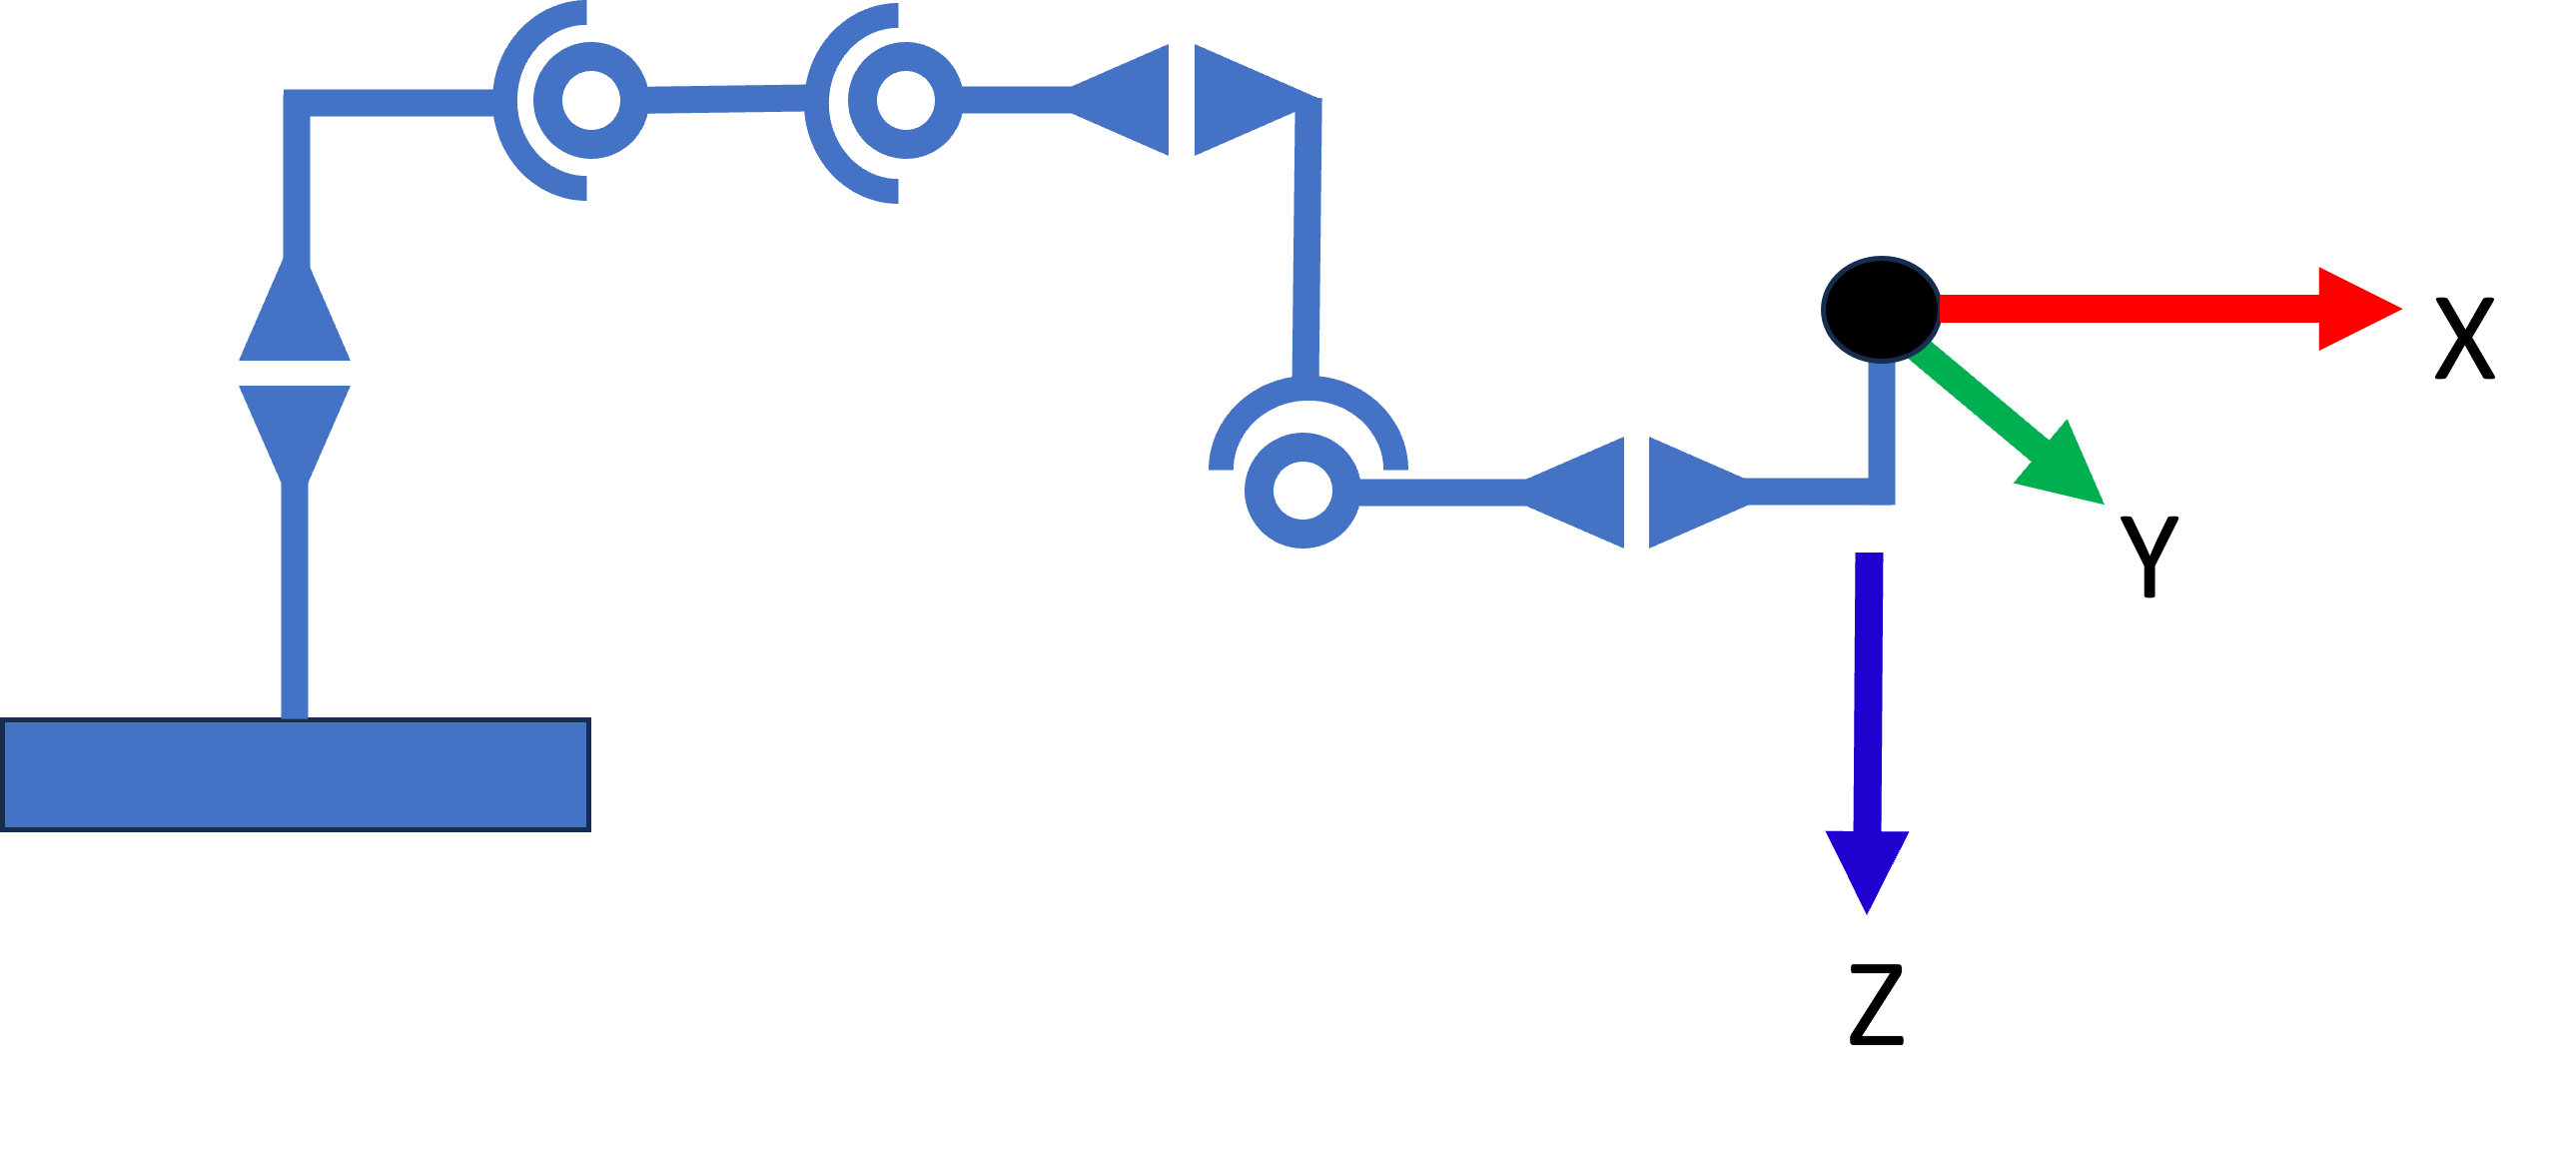
\includegraphics[width=0.7\textwidth]{figures/schema.png}}
	\caption{Schematics of the modeled robot}
	\label{schema}
\end{figure}

The next step is to model a spindle that is attached to the flange, which is at the end of the last link and apply a transformation matrix from the flange to the tip of the end-mill.
Figure~\ref{robotprog} depicts the robot modeled using Python in combination with the \textit{Matplotlib} library. The joint positions, in degrees, are as follows: [0, 135, -45, 0, 0, 0], corresponding to joints 1 to 6, respectively. The colored arrows shown in the figure represent the coordinate axes of the \acrshort{TCP}. The X-axis of the \acrshort{TCP} coordinate system is represented in red, while the Y-axis and Z-axis are denoted by the colors green and blue, respectively. To distinguish the \acrshort{TCP} coordinate system from the world coordinates system, the \acrshort{TCP} coordinates system axes are marked with a dash. The first link of the robot, originating from the point X=0, Y=0, Z=0 in the world coordinate system, is displayed in green. The individual joints are represented by red dots. The end-mill is marked as a orange dot.


\newpage
 \begin{figure}[H]
	\centerline{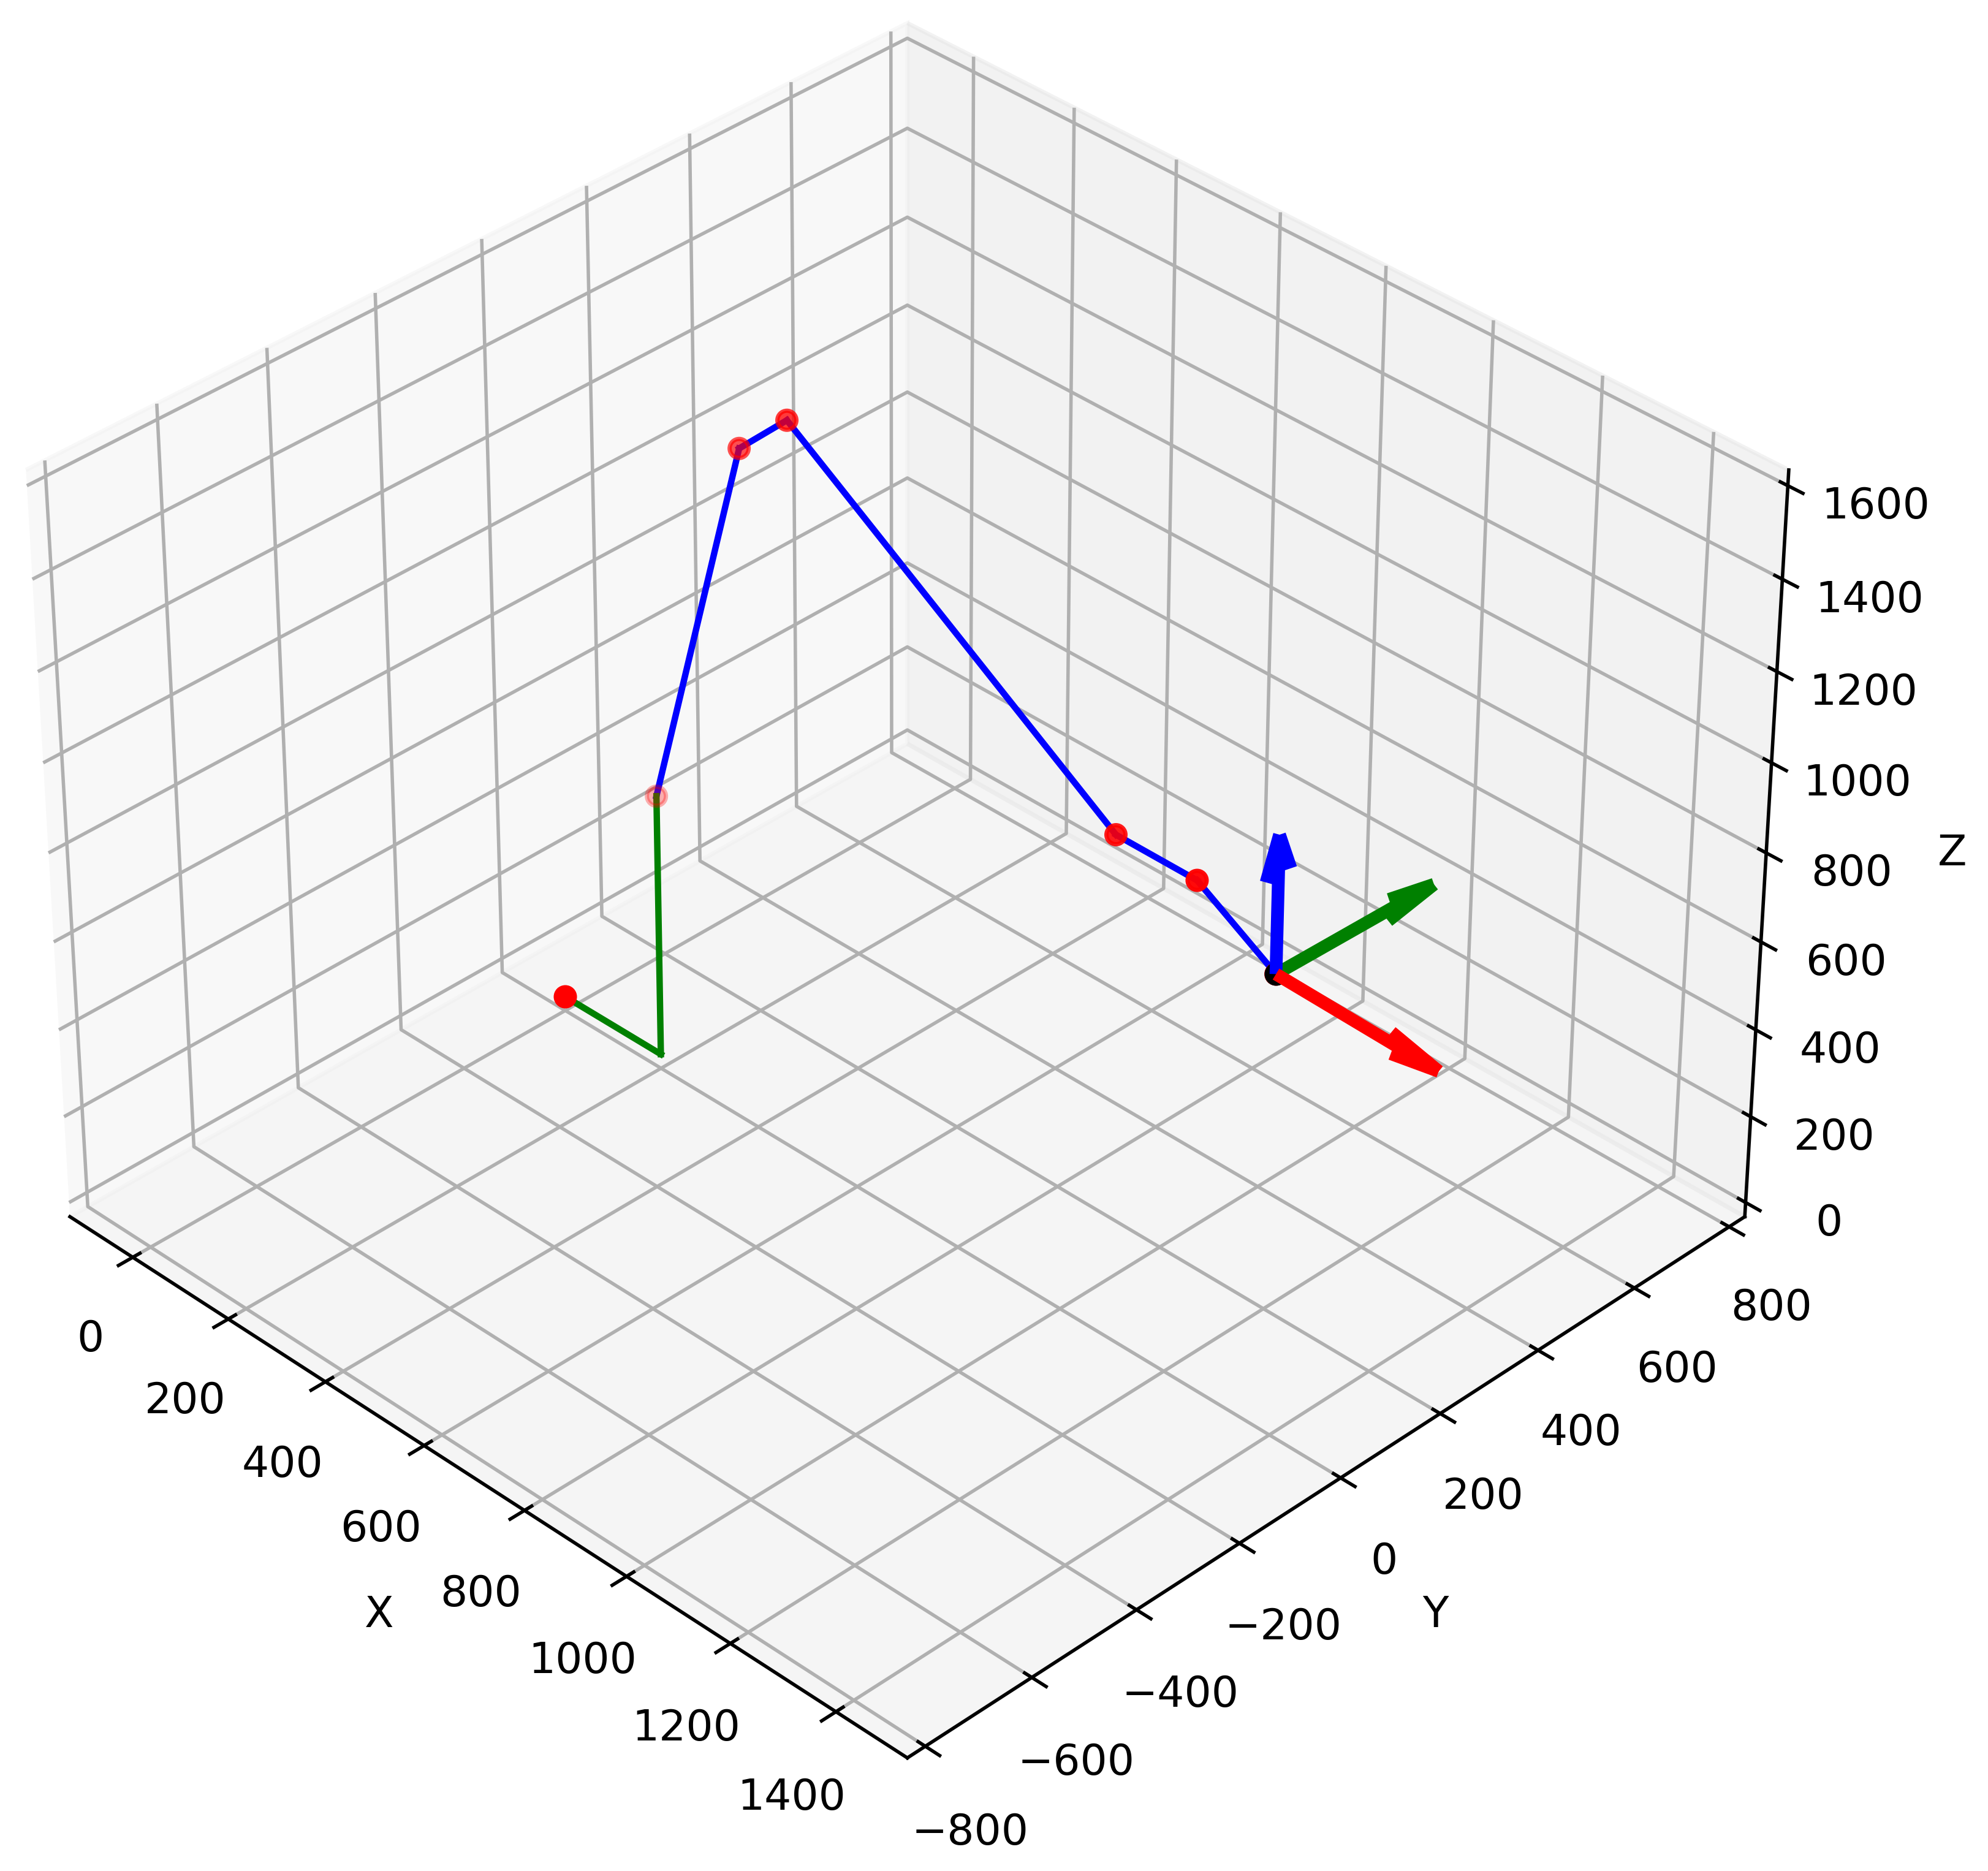
\includegraphics[width=1\textwidth]{figures/robotprog.png}}
	\caption{Visualization of the modeled robot in Python}
	\label{robotprog}
\end{figure}


\subsection{Modeling a Basic Toolpath}\label{MBT}
Before analyzing the process variables, it is necessary to define a toolpath for the \acrshort{TCP} to follow. For that case, three options are presented, each consisting of 3000 coordinates. It should be noted that the redundant \acrshort{DoF} in these cases is the rotation around the Z-axis. This rotation will be adjusted to determine the optimal value for the desired outcome. A and B are held at 0°.

The first toolpath, depicted in Figure \ref{path1}, represents a converging spiral that is shifting to the side. Figure \ref{path2} illustrates a converging-diverging infinity-loop, and Figure \ref{path3} displays a forward-moving sinusoidal curve that is following a parabolic profile. Each path consists out of 3000 coordinates. %The corresponding equations for these toolpaths are given by Equation \ref{eq1}, Equation \ref{eq2}, and Equation \ref{eq3}, respectively. The variable \textit{iter} ranges from 0 to 3000 and is used to calculate the X, Y, and Z coordinates. Trigonometric functions are utilized with the help of the \textit{Numpy} library. Currently, no rotation (A, B, or C) has been defined. Only the coordinates are specified. Each toolpath has specific dimensions and characteristics. 

Figure \ref{TP1robot} illustrates the robot and Toolpath 1 at the final position of the toolpath. The origin of the toolpath is shifted by X=+800 and Z=+400 relative to the world coordinate system. No rotations are applied around the X, Y, and Z axes, resulting in A, B, and C being zero. As a result, the coordinate axes of the \acrshort{TCP} are parallel to the axes of the world coordinate system.

\begin{figure}[H]% [H] is so declass\'e!
	\centering
	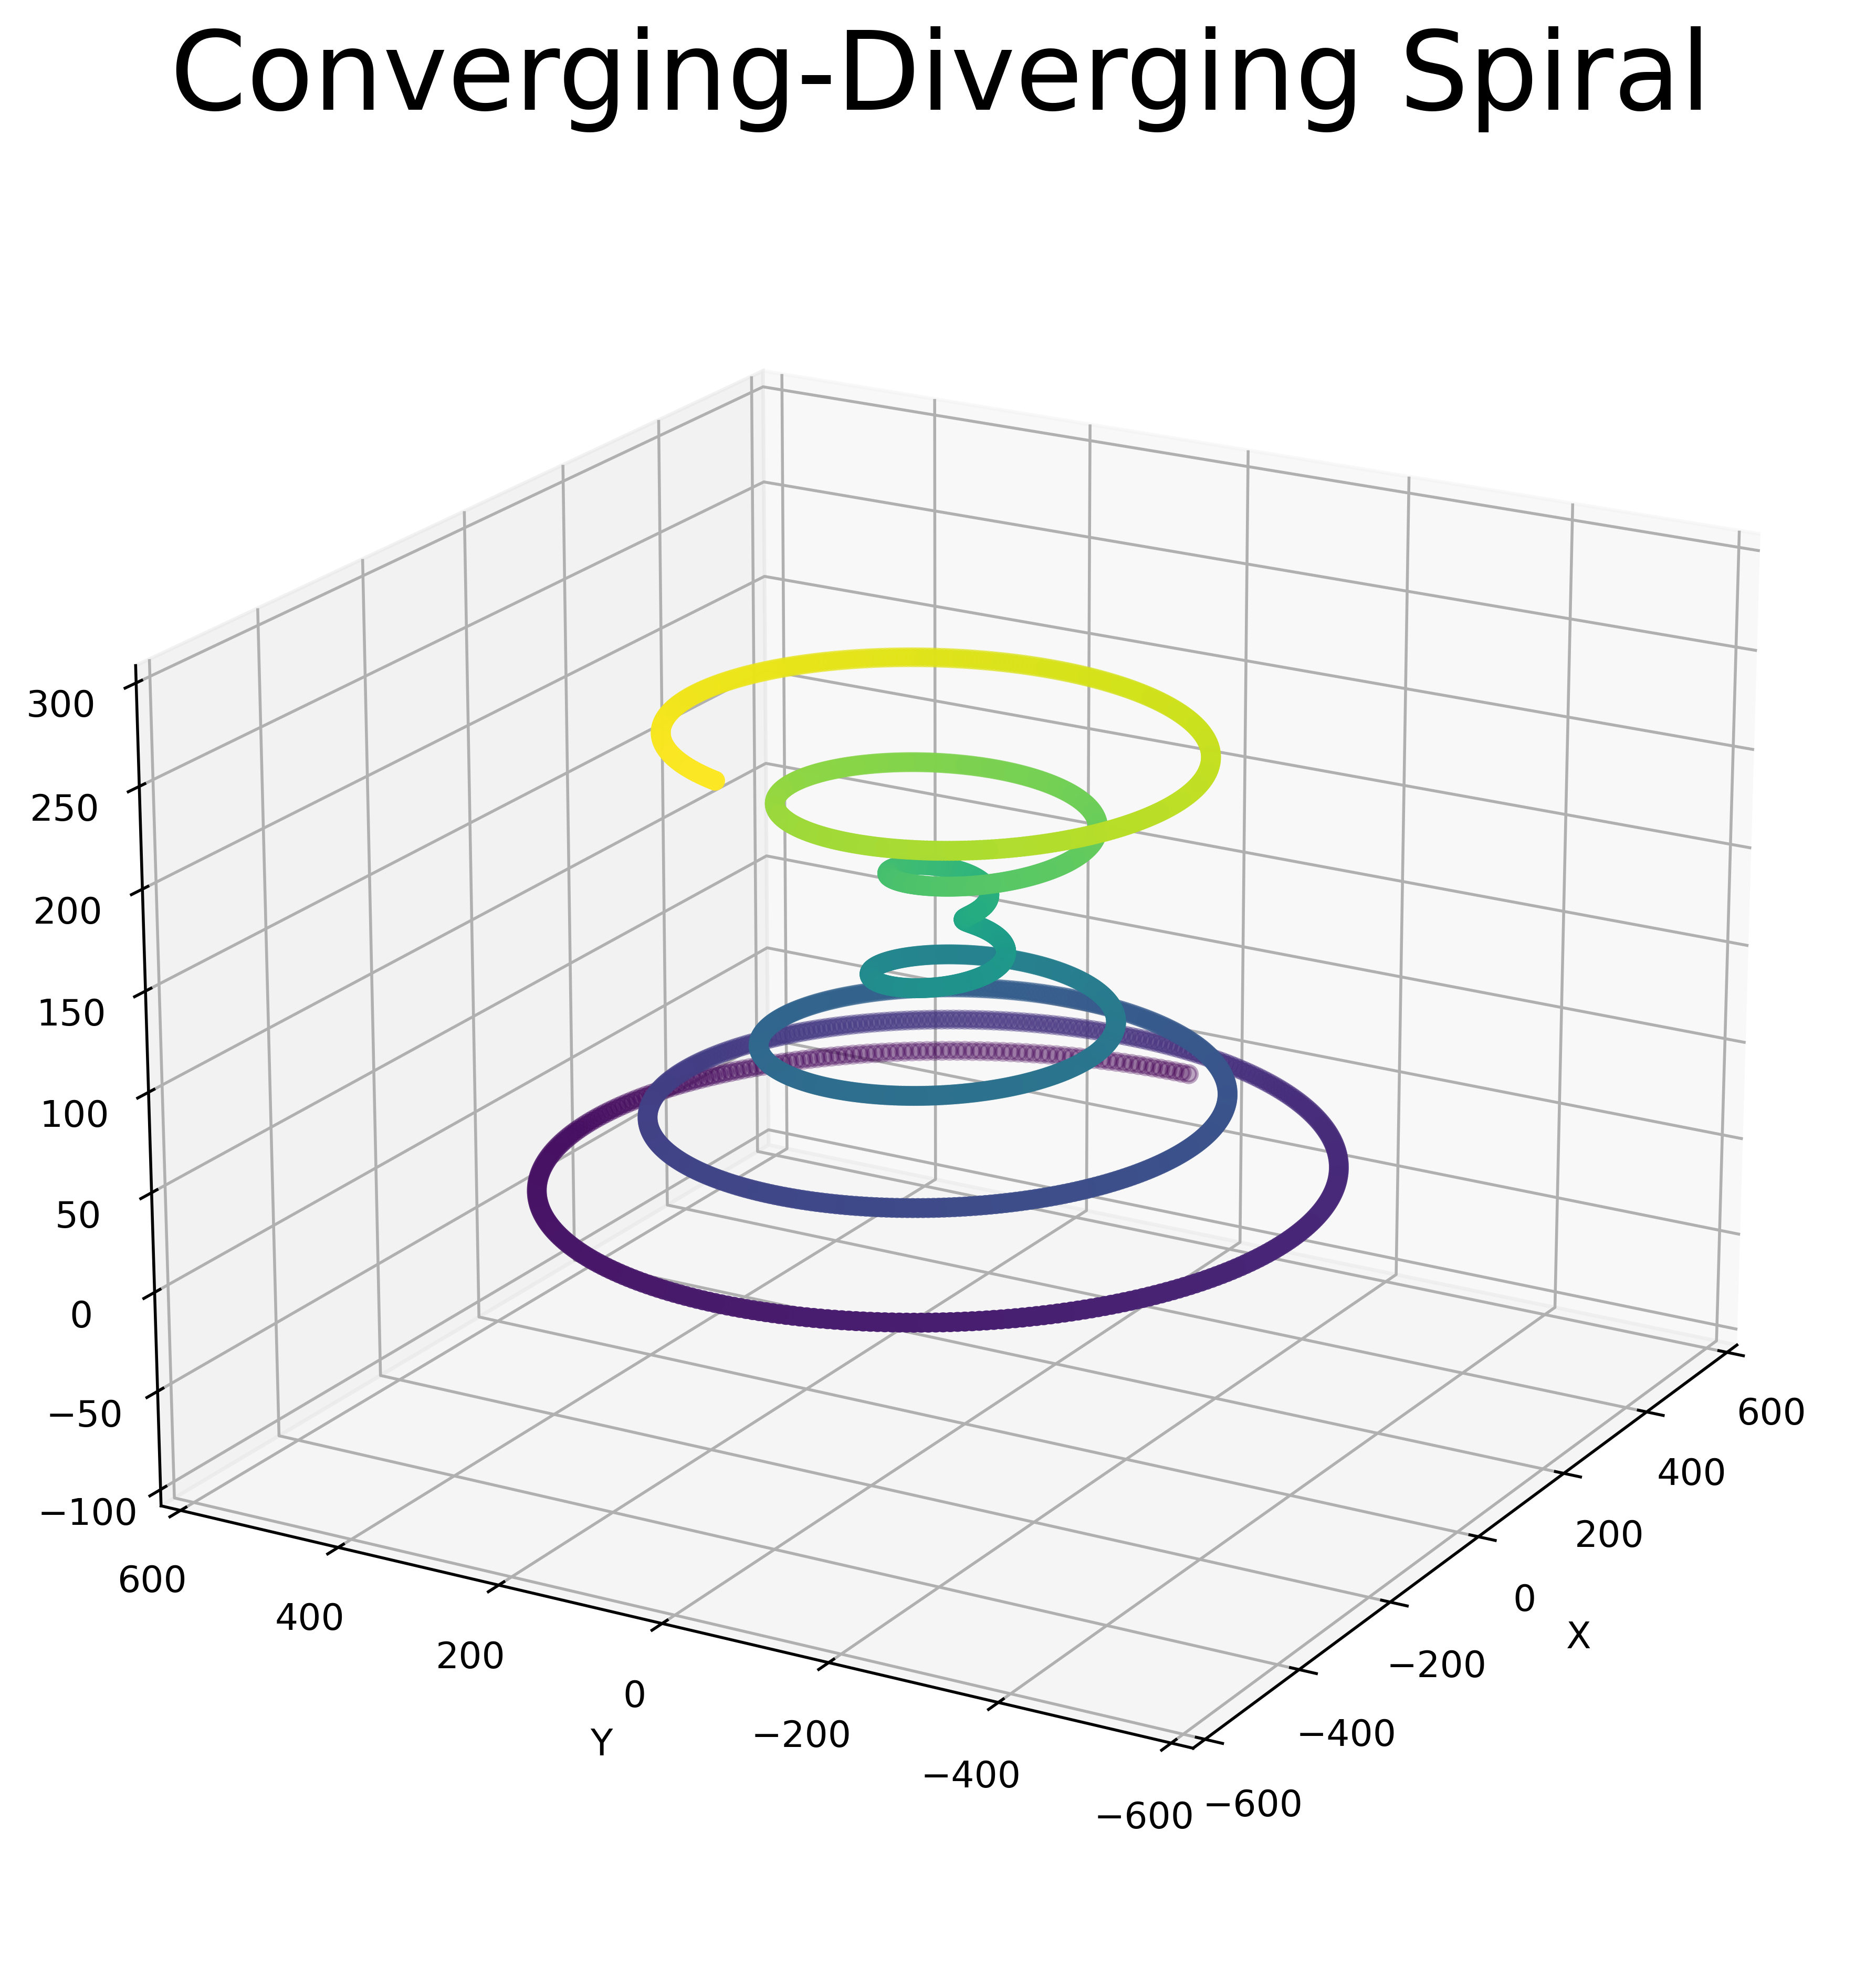
\includegraphics[width=0.6\textwidth]{figures/path1.png}
	\caption{Toolpath 1: Converging spiral}
	\label{path1}
\end{figure}

%\begin{equation}\label{eq1}
%	\begin{split}
%		x &= cos(iter) * (500 - iter / 3) + iter/10\\
%		y &= sin(iter) * (500 - iter / 3) + iter/10\\
%		z &= iter / 6
%	\end{split}
%\end{equation}

\begin{figure}[H]% [H] is so declass\'e!
	\centering
	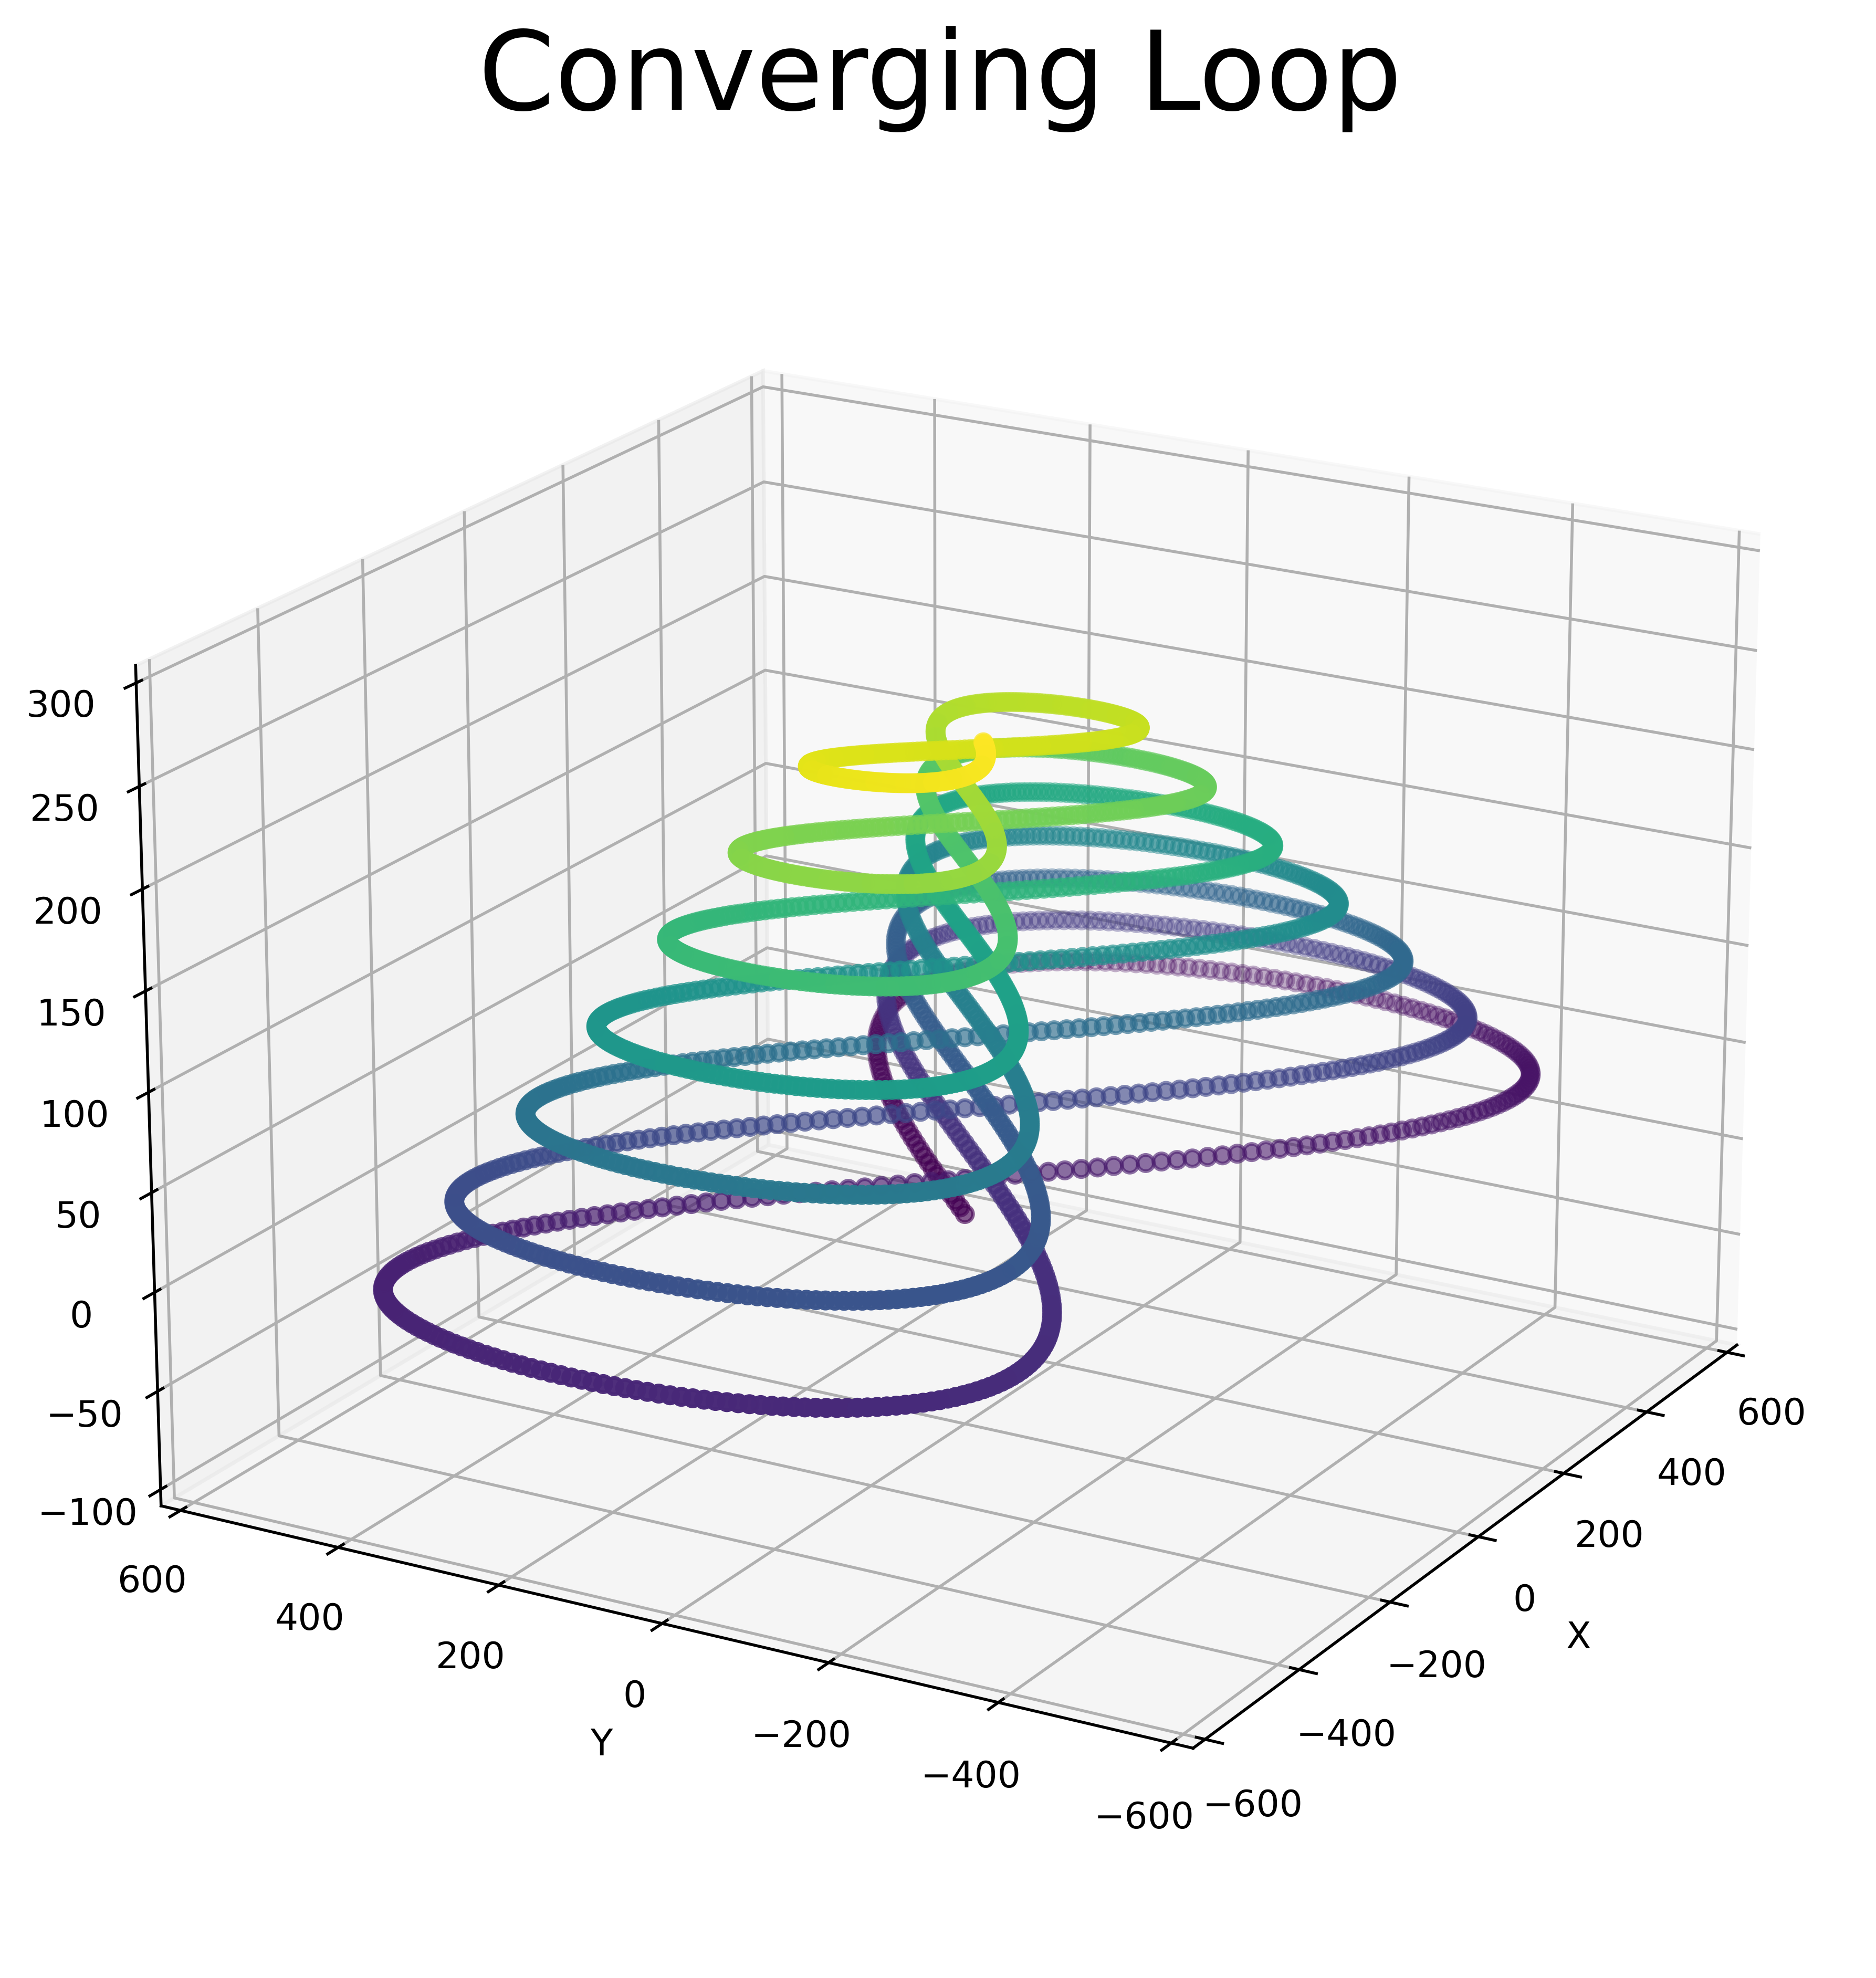
\includegraphics[width=0.6\textwidth]{figures/path2.png}
	\caption{Toolpath 2: Converging infinity loop}
	\label{path2}
\end{figure}
\newpage
%\begin{equation}\label{eq2}
%	\begin{split}
%		x &= sin(iter) * cos(iter) * (500-iter / 6)\\
%		y &= sin(iter) * (400-iter / 5)\\
%		z &= iter / 10
%	\end{split}
%\end{equation}




\begin{figure}[H]% [H] is so declass\'e!
	\centering
	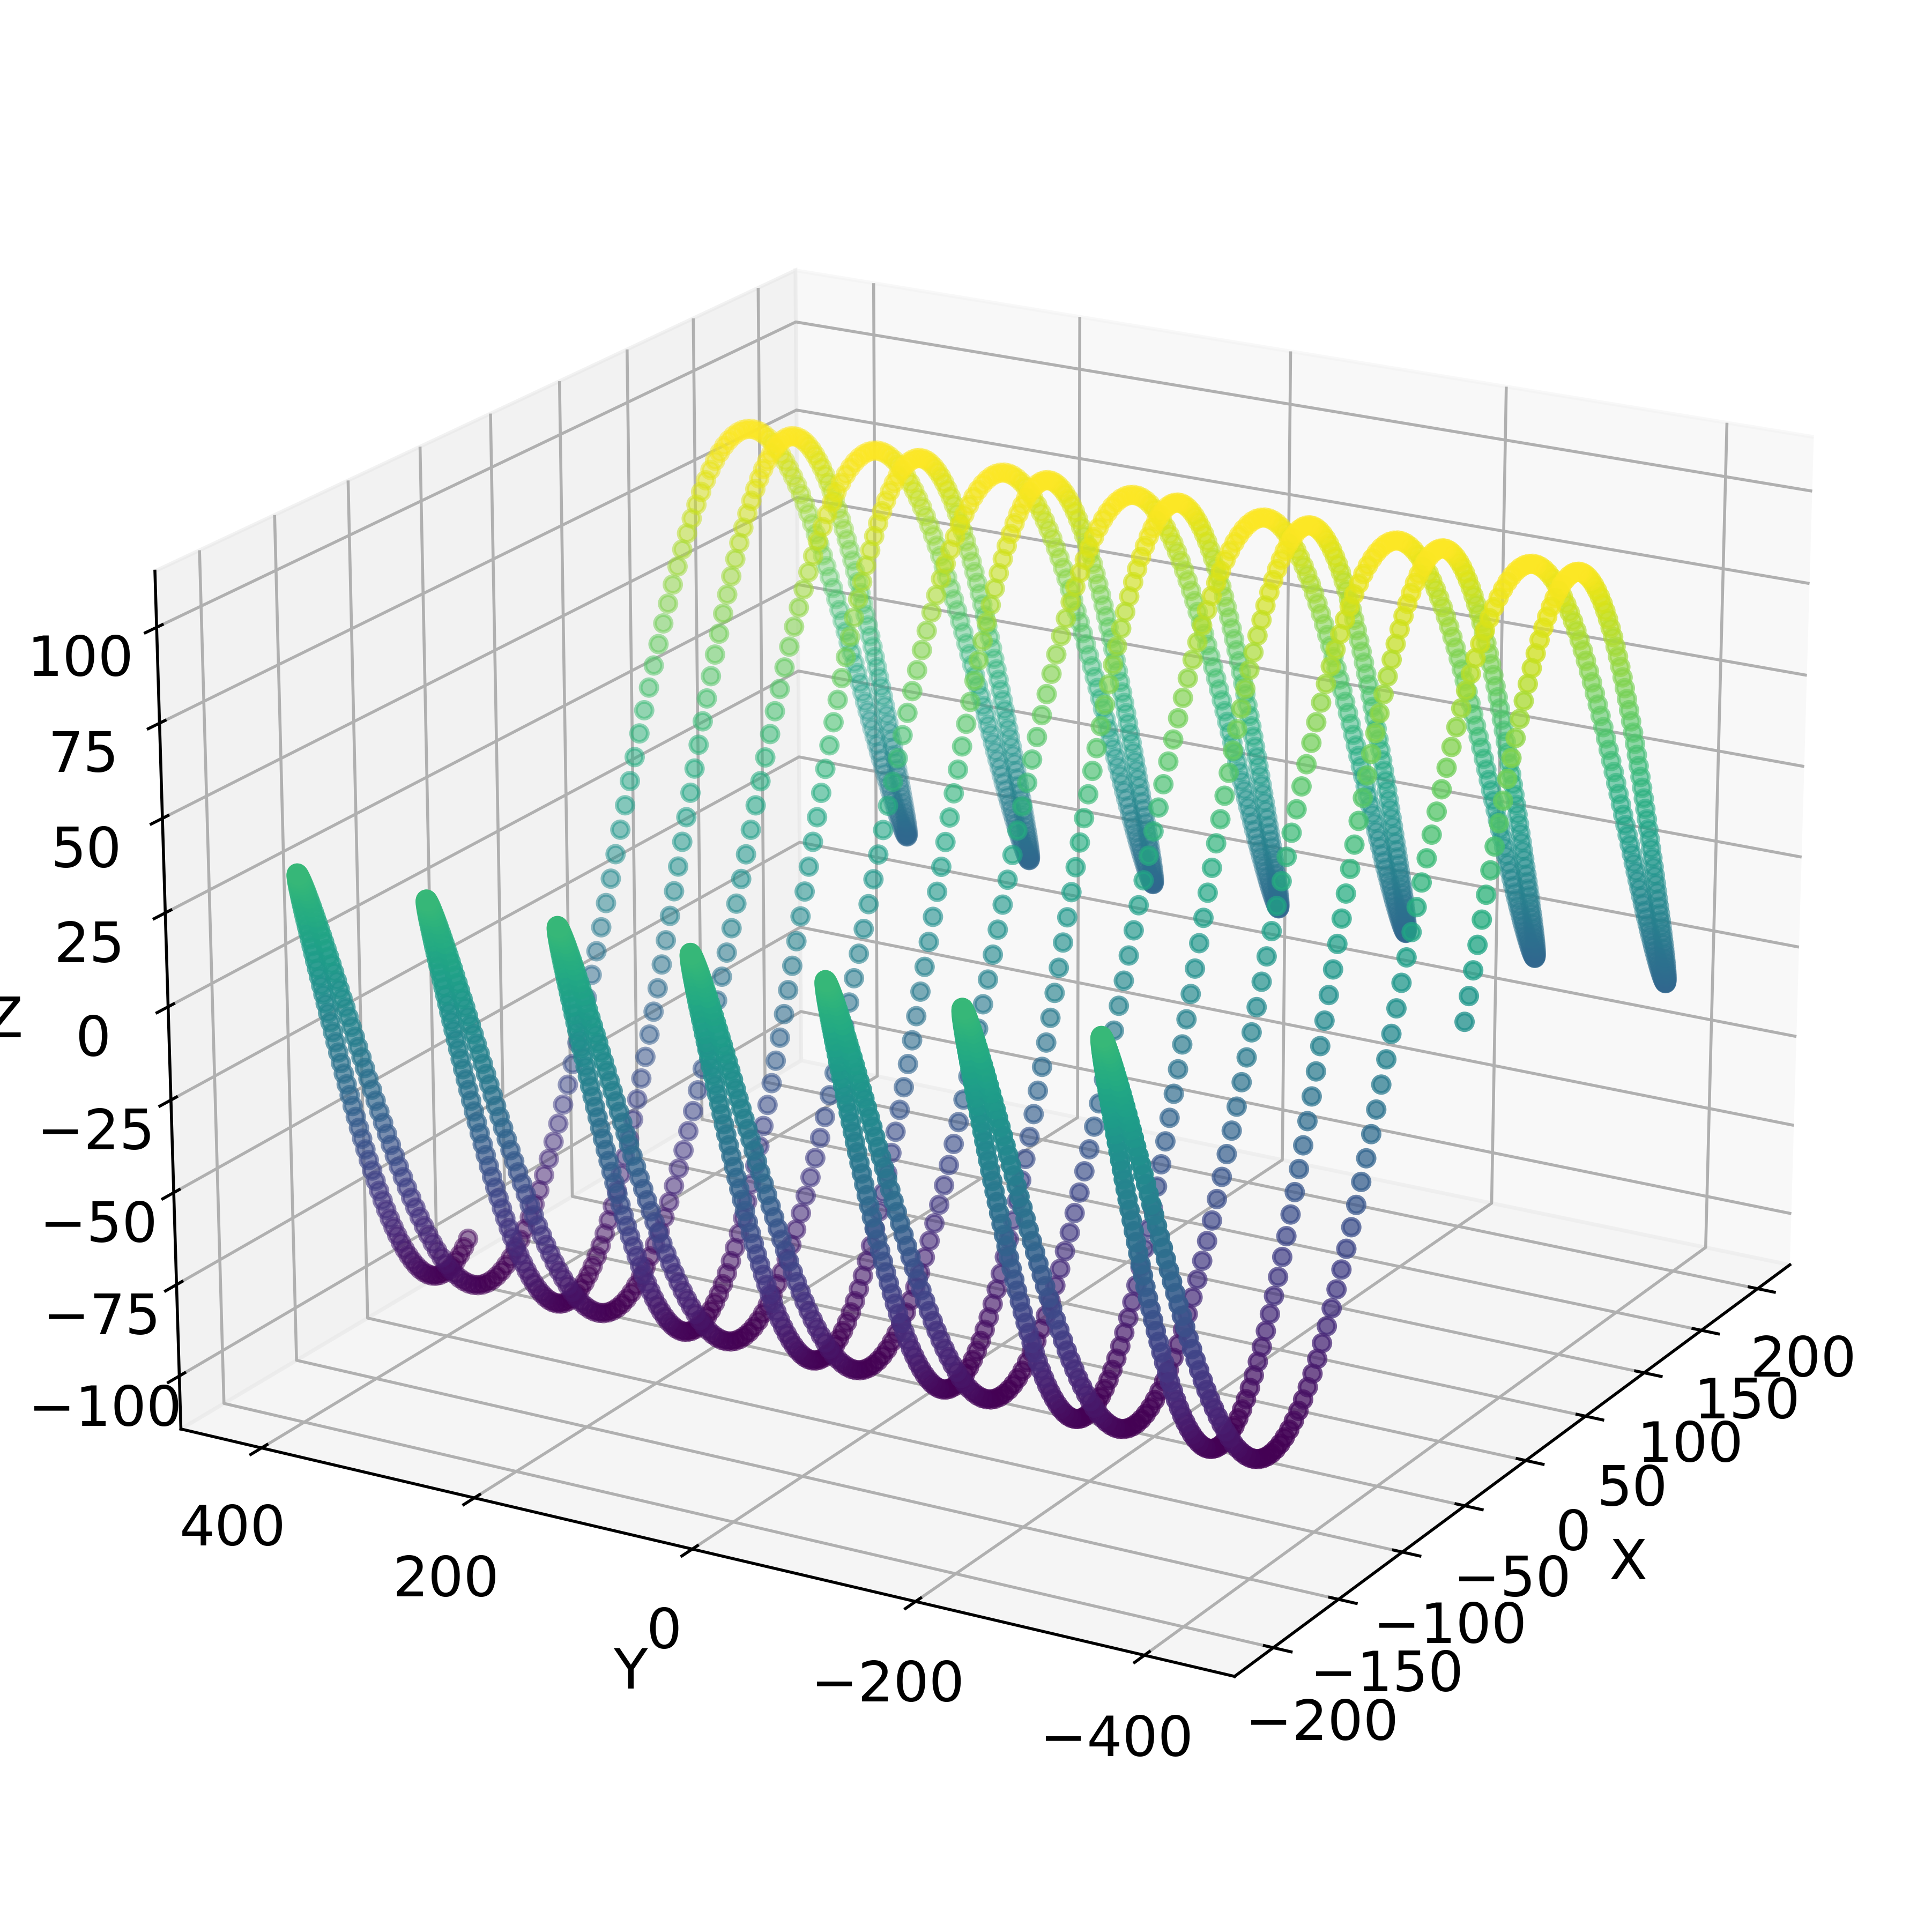
\includegraphics[width=0.6\textwidth]{figures/path3.png}
	\caption{Toolpath 3: Forward moving pendulum oscillation}
	\label{path3}
\end{figure}
%\begin{equation}\label{eq3}
%	\begin{split}
%		x &= sin(iter) * 200\\
%		y &= (iter / 3) - (2500/6)\\
%		z &= sin(x)*100 + (iter**2)/35000
%	\end{split}
%\end{equation}







\begin{figure}[H]
	\centerline{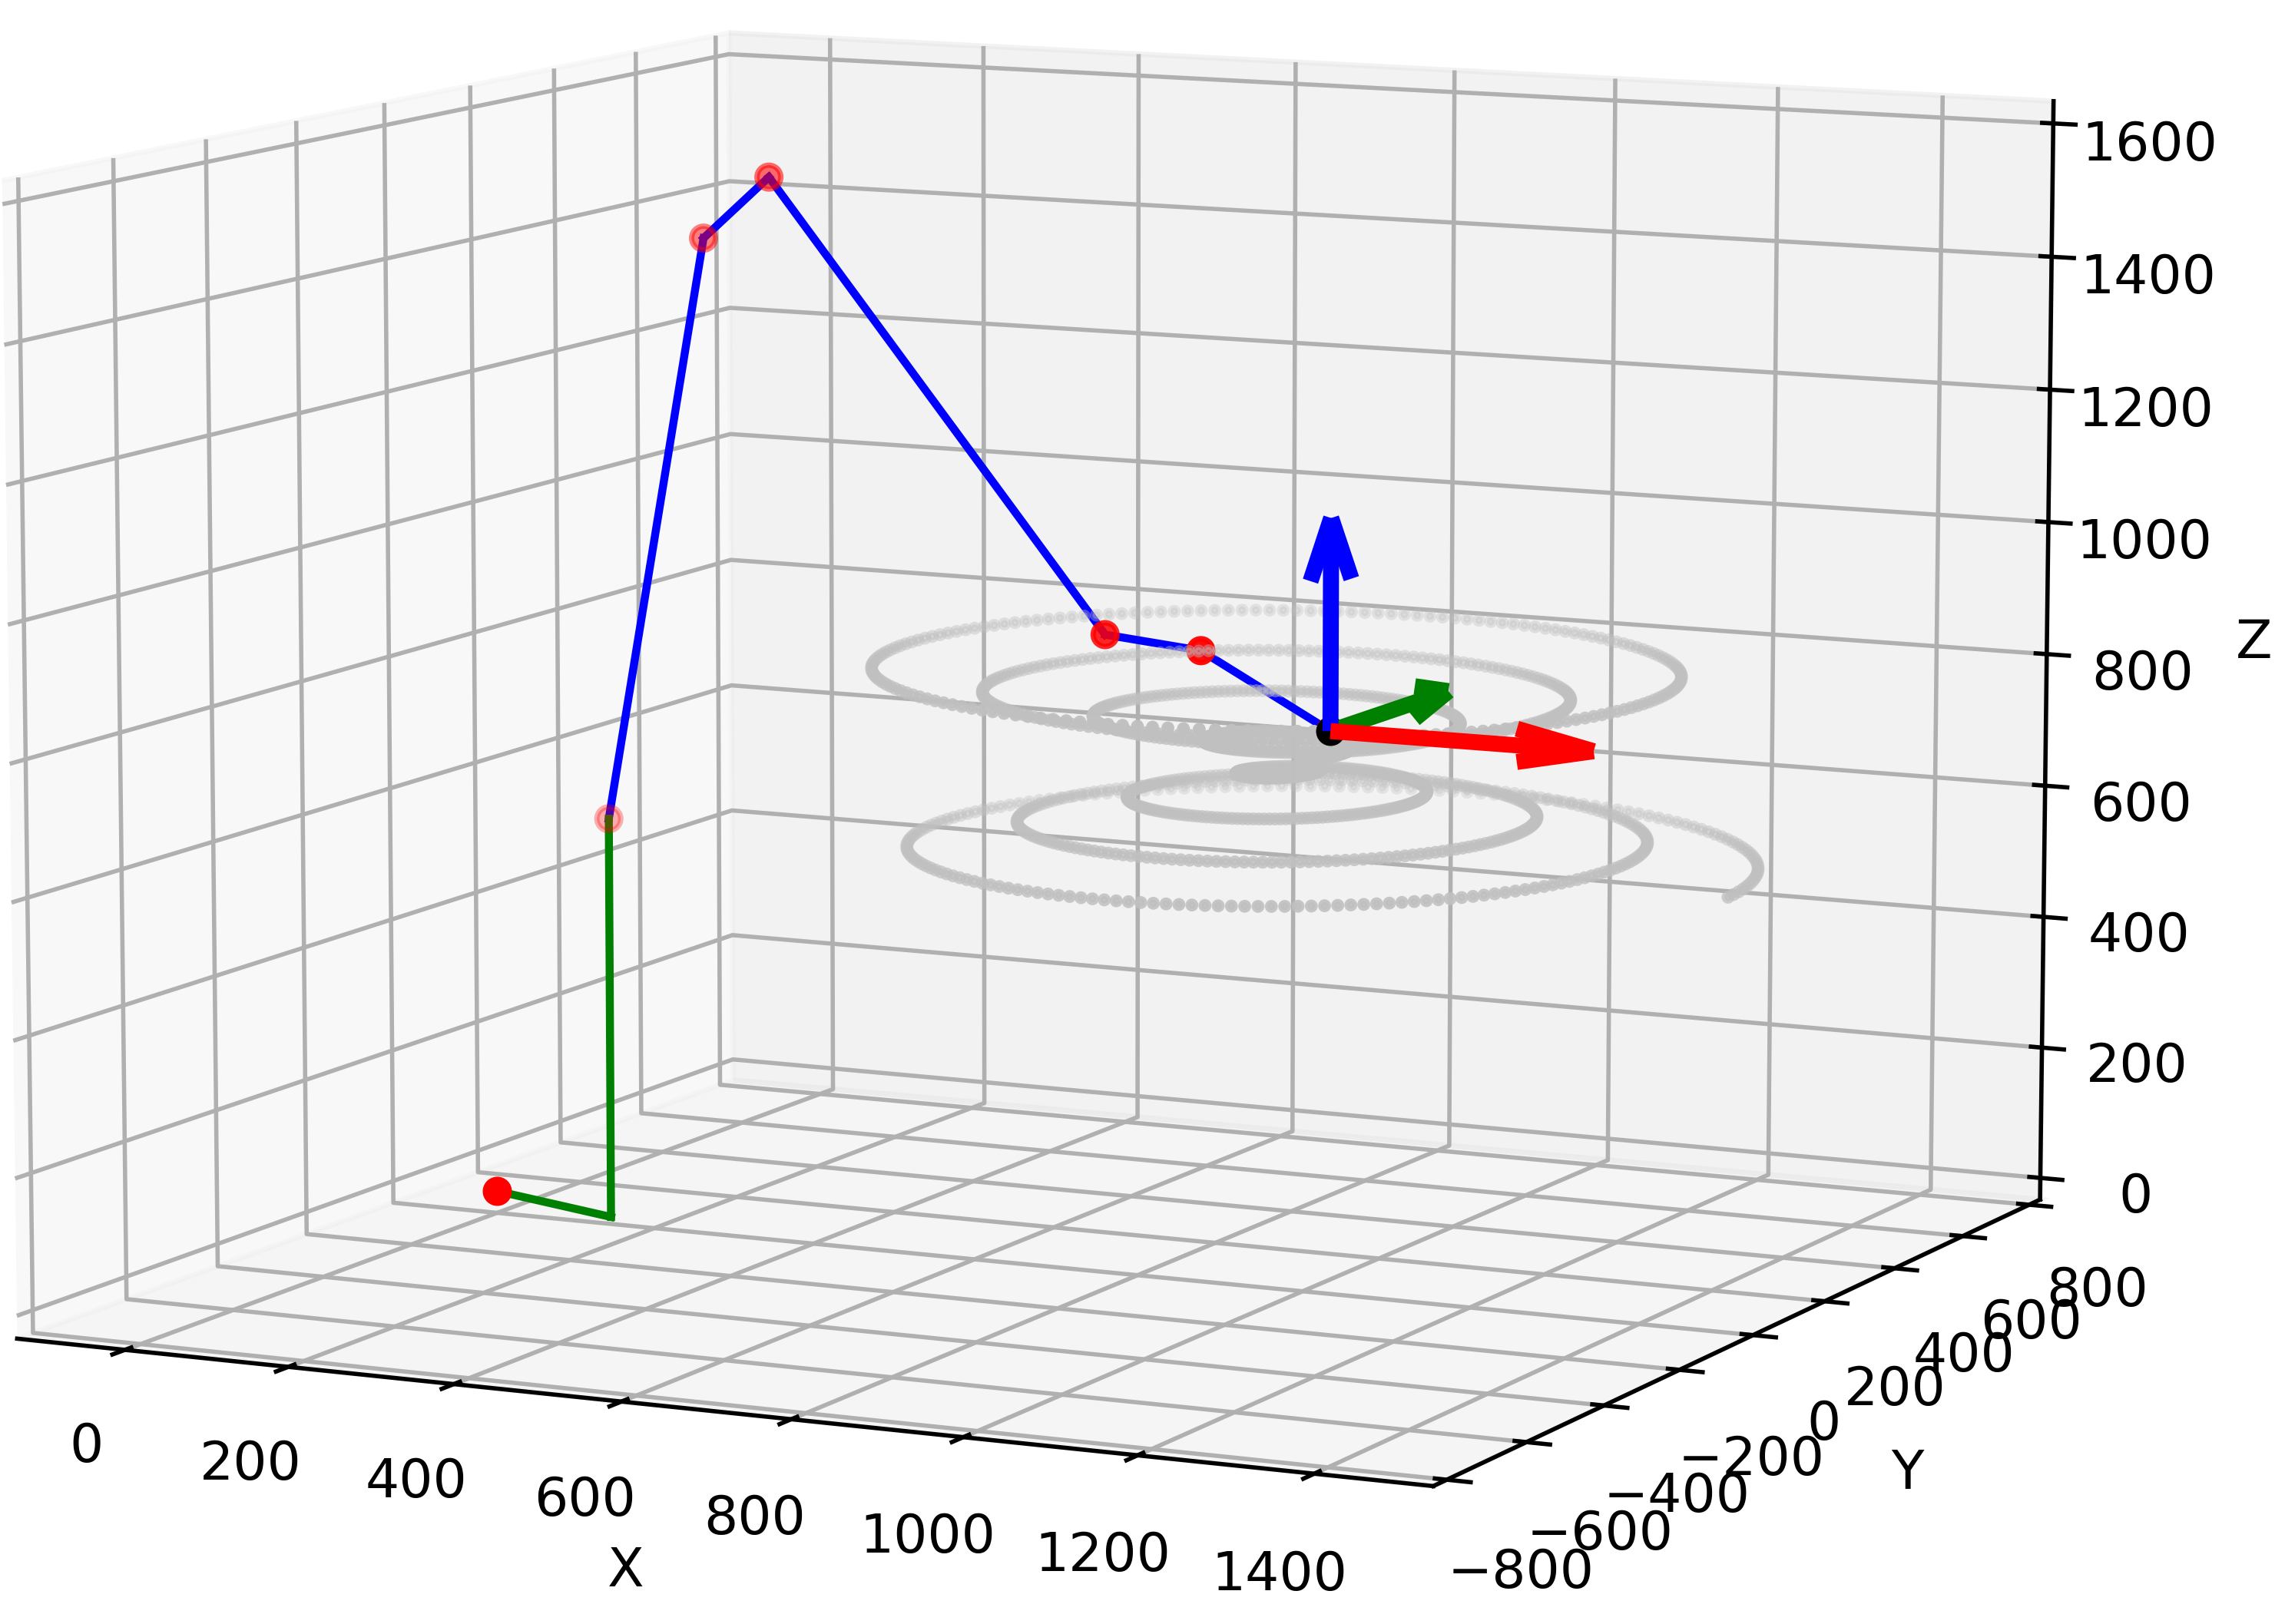
\includegraphics[width=0.9\textwidth]{figures/robotANDpath1.png}}
	\caption{Traversing toolpath 1}
	\label{TP1robot}
\end{figure}




\subsection{Extracting Process Variables}
By utilizing the inverse kinematics algorithm from the Python library \textit{visual\_kinematics}, the joint angles for each coordinate can be computed. To achieve this, the rotations A, B, and C need to be defined. The outcome is a time-series that contains the corresponding joint positions. For all tests, all coordinates must be traversed in equidistant time steps. With this information, it becomes possible to calculate the velocity and other related variables. By transforming all the data from the time-series into scalar values and calculating the local rating, the local and global scores can be determined.

\section{Testing and Validation}%

\subsection{Toolpath Evaluation With one Redundant DoF}
%\subsubsection{Obtaining Joint Positions}
As discussed in Chapter \ref{MBT}, the toolpath remains constant with respect to the X-, Y-, and Z-coordinates. The fixed boundary conditions for the robot are that there are no rotations around the X and Y axes, resulting in A and B both being equal to zero. This condition is fixed for the entire toolpath. The user has the ability to set the \acrshort{DoF} for the rotation around the Z-axis, which is the redundant \acrshort{DoF}. Figure \ref{TP1ABC0} displays the variation of each joint over time for toolpath 1. In this specific case, the rotations A, B, and C are all set to 0. The entire toolpath is traversed in 300 seconds.

\begin{figure}[H]
	\centerline{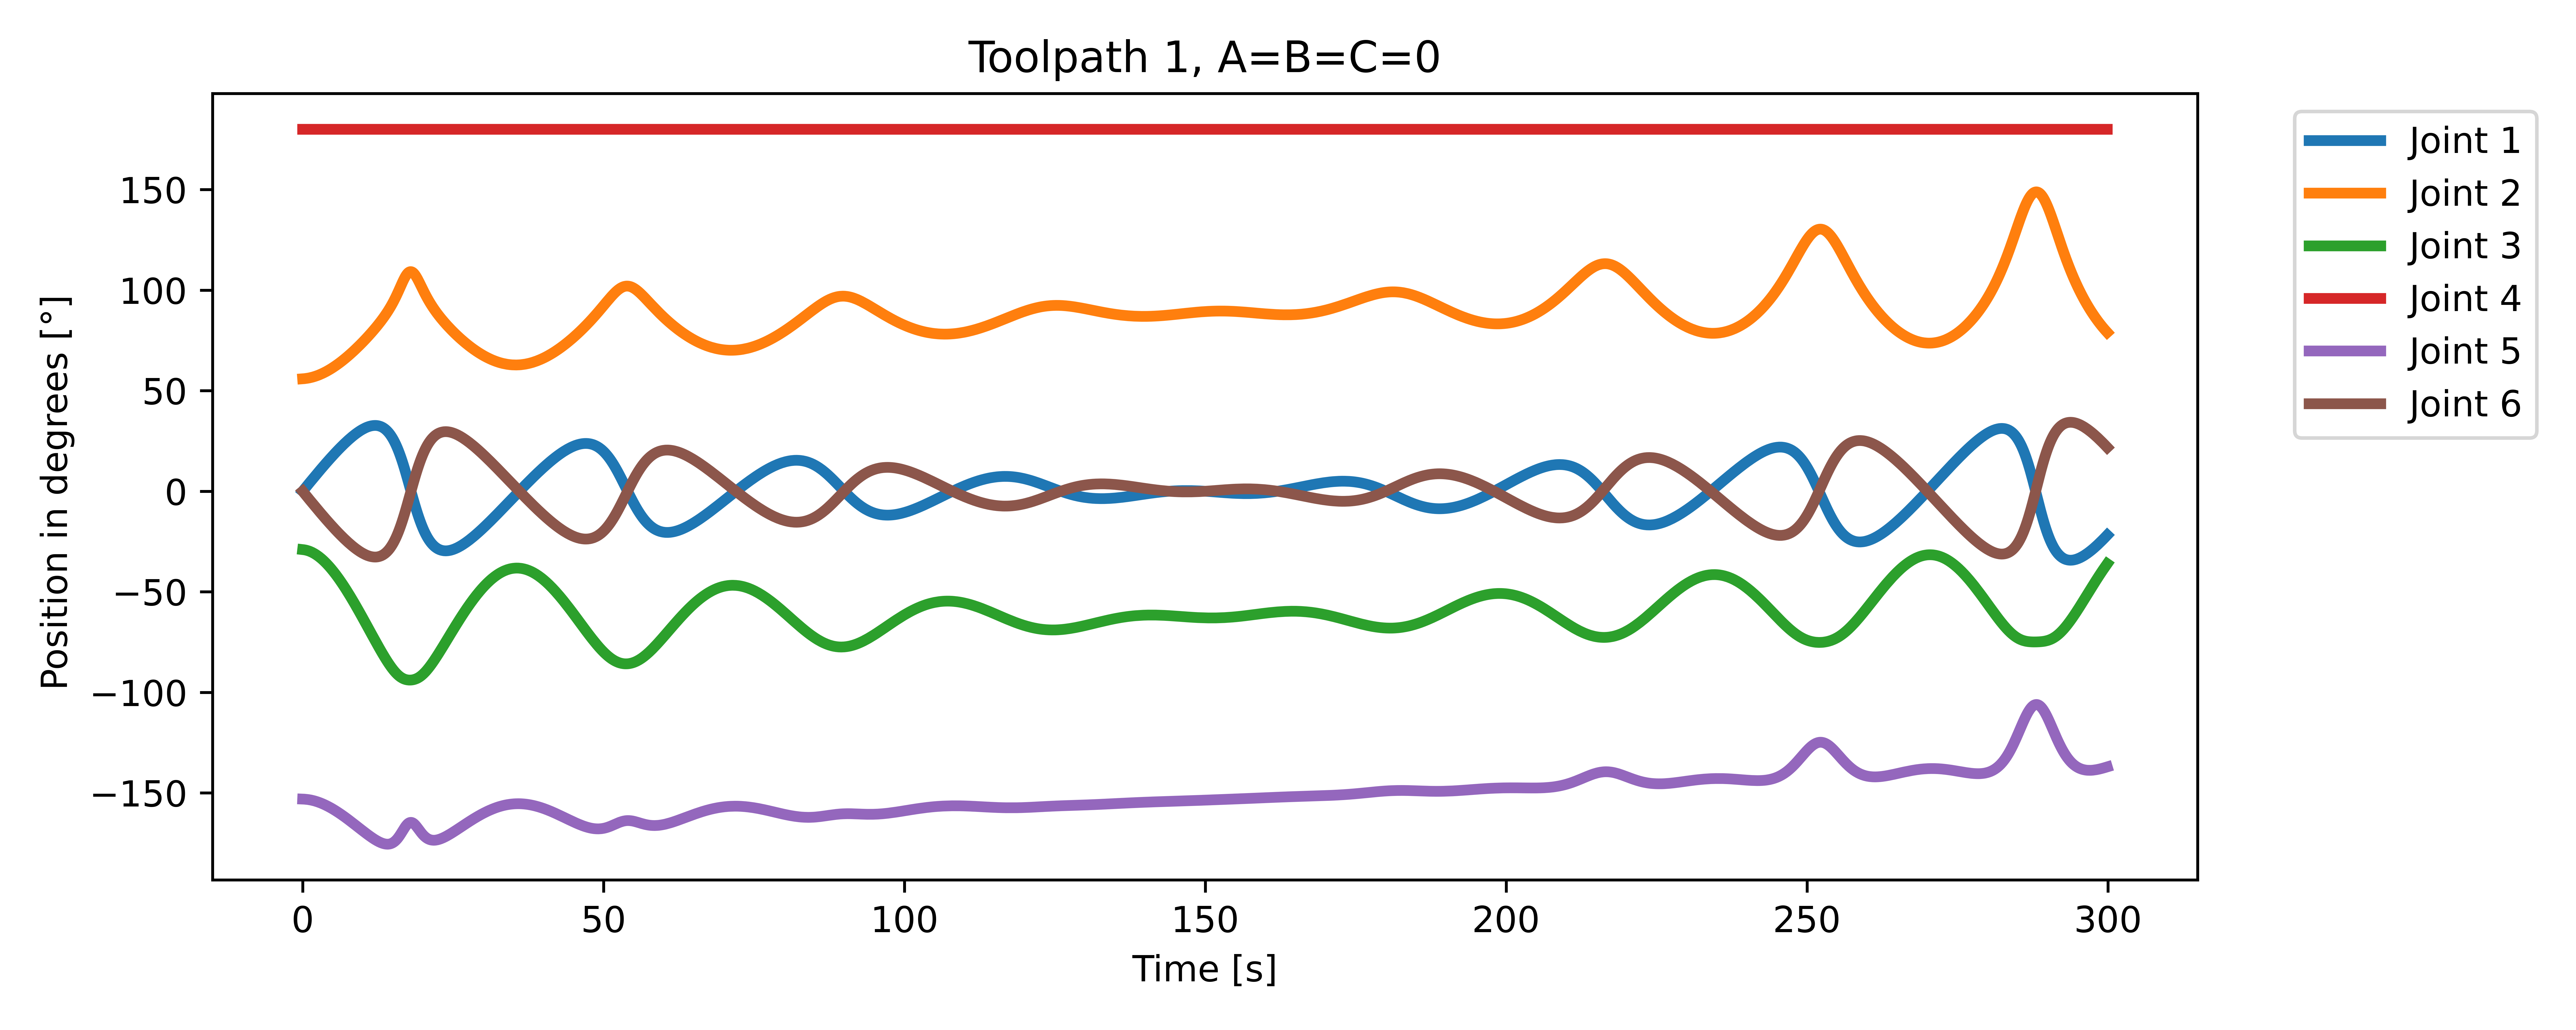
\includegraphics[width=1\textwidth]{figures/TP1ABC0.png}}
	\caption{Visualization of the joint positions over time for toolpath 1 with C=0°}
	\label{TP1ABC0}
\end{figure}

Figure \ref{TP1ABC45} depicts the joint positions for all six joints over time for the same toolpath (toolpath~1) with a 45° rotation around the Z-axis (C = 45°). 
\begin{figure}[H]
	\centerline{\includegraphics[width=1\textwidth]{figures/TP1ABC45.png}}
	\caption{Visualization of the joint positions over time for toolpath 1 with C=45°}
	\label{TP1ABC45}
\end{figure}

It is noticeable that joint 4 and joint 5 have experienced changes in their respective ranges. Furthermore, joint 6 exhibits a significantly larger amplitude towards the end of the toolpath, in comparison to the case with no rotation (C=0°).

Figure \ref{TP1ABC0} illustrates the variations in each joint over time for toolpath 2 (Eq. \ref{eq2}) without any rotation (A=B=C=0°). Unlike toolpath 1, the amplitudes notably decrease towards the end of the toolpath. This observation aligns with the unique characteristics of different toolpaths.
 
 %In this case all joints show a oscillation except joint 4.
\begin{figure}[H]
	\centerline{\includegraphics[width=1\textwidth]{figures/TP2ABC0.png}}
	\caption{Visualization of the joint positions over time for toolpath 2}
	\label{TP2ABC0}
\end{figure}

%ToDo: EXPLAIN WHY JOINT 4 IS AT 180 all the time!!!!!!!!\newline
%\subsubsection{Selecting Process Parameters}
The next step involves selecting the process variables of interest and assigning weights to each variable. For this purpose, a basic case is discussed. The selected process variables are listed in Table \ref{PPbasic}. The total number of direction changes in all joints and the total distance traveled are chosen due to their ease of implementation. The number of direction changes is assigned an importance factor of 0.2.
The total travel in all joints is combined and given an importance factor of 0.4.
Additionally, the acceleration of joint 1 is analyzed. To obtain a scalar value for the acceleration, the individual acceleration values are squared and then summed up. The importance factor for acceleration in joint 1 is 0.4. Other process variables are disregarded.

\begin{table}[H]
	\centering
	\begin{tabular}{||l|l||}
		Process variables& Importance factors \\
		\hline
		\hline
		\hline
		Direction changes in joints 1-6	&		0.2 \\
		Total travel in joints 1-6	&  	0.4 \\
		Acceleration in joint 1	& 		0.4\\
		
		\hline
		\hline
	\end{tabular}
	
	\caption{Selected process variables and their importance factors}
	\label{PPbasic}
\end{table}


Since only one redundant \acrshort{DoF} is being analyzed, it is possible to represent the individual local scores and global score as a one-dimensional graph. Firstly, toolpath 1 is analyzed by incrementing the redundant \acrshort{DoF} (C-axis) by 5 degrees, starting from -135 degrees and ending at 135 degrees.


Figure \ref{TP1-25} illustrates a case with a -45° rotation around the Z-axis for toolpath~1.
Similarly, Figure \ref{TP1+25} displays a case with a +45° rotation around the Z-axis for toolpath~1.

\begin{figure}[H]
	\centering
	\begin{minipage}{0.5\textwidth}
		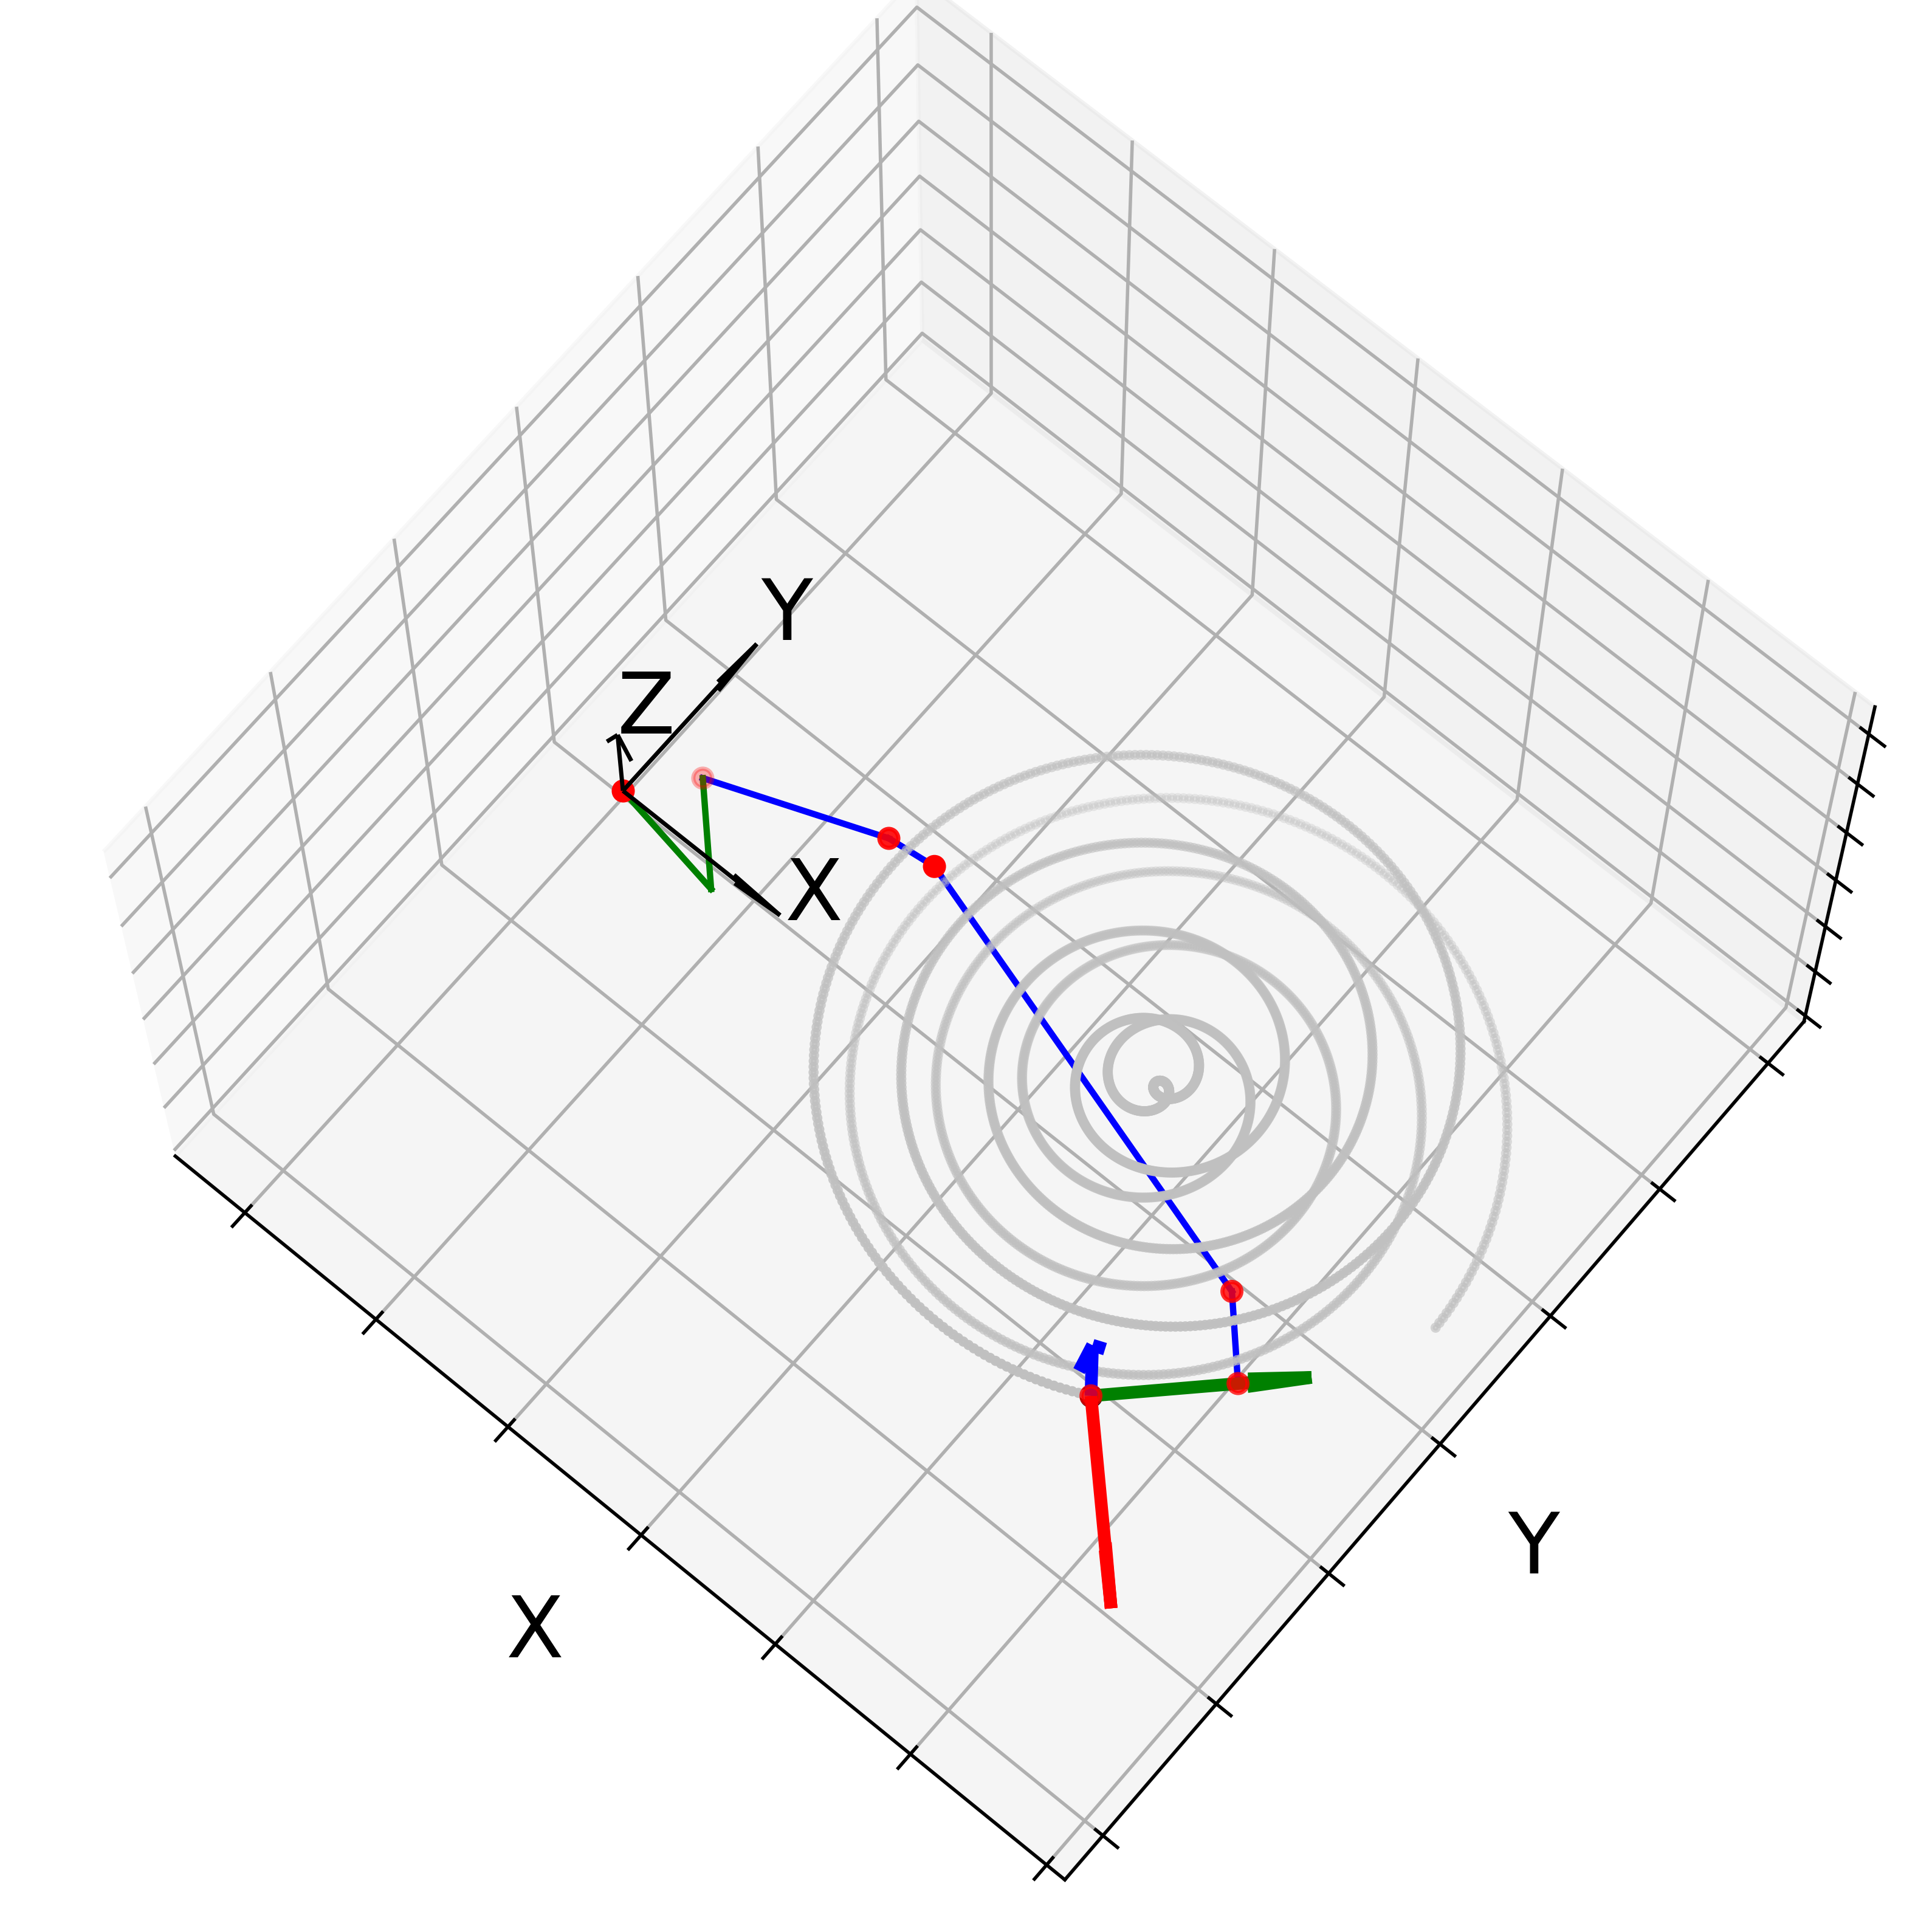
\includegraphics[width=\textwidth]{figures/robotANDpath1_-45.png}
		\caption{Toolpath 1 with A=0°, B=0° and C=-45°}
		\label{TP1-25}
	\end{minipage}\hfill
	\begin{minipage}{0.5\textwidth}
		\includegraphics[width=\textwidth]{figures/robotANDpath1_45.png}
		\caption{Toolpath 1 with A=0°, B=0° and C=45°}
		\label{TP1+25}
	\end{minipage}\par
\end{figure}

A total of 55 time-series of joint positions are generated. On average, the inverse kinematics algorithm takes 35 seconds to calculate the joint values for all 3000 coordinates. The process variables are extracted and scaled in relation to each other, as described in Chapter~\ref{LRC}. It is important to note that before scaling, the selected process variables are pre-multiplied by -1, as each value should be minimized. The arrays of local ratings are then multiplied by the weights selected in Table \ref{PPbasic}. Subsequently, the local scores of each process variable can be plotted as a one-dimensional graph, as shown in Figure \ref{LS1}.

\begin{figure}[H]
	\centerline{
\includegraphics[width=1\textwidth]{figures/LocalScores_1.png}}
	\caption{Local scores of each process variable for toolpath 1}
	\label{LS1}
\end{figure}
\newpage
The acceleration in joint 1 and the combined total travel in the joints exhibit a smooth oscillating curve with a decreasing amplitude towards the positive end of the analyzed range. It is worth mentioning that the maximum value that the local score can reach is 40 for acceleration and total travel, while for direction changes, the maximum score is 20. This is due to the assigned importance factors. The direction changes display a less smooth, but still oscillating trajectory.

Next, the local scores are summed up to calculate the global score. The resulting array, displayed in Figure \ref{GS1}, represents the global score achieved by varying the rotation around the Z-axis in relation to all other analyzed values. The green cross on the graph indicates the maximum attainable score and its corresponding rotation, compared to all analyzed boundary conditions.

\begin{figure}[H]
	\centerline{\includegraphics[width=1\textwidth]{figures/best_c_1.png}}
	\caption{Global score for toolpath 1}
	\label{GS1}
\end{figure}
In this particular case, the highest achievable score is 91.1 at -120 degrees. This nearly perfect score indicates that setting the rotation to -120 degrees results in minimal direction changes, minimal total travel, and close to minimal acceleration in joint 1. It is crucial to emphasize that this rating is only in comparison to the other analyzed boundary conditions.

The same analysis, using identical process variables and weights, can be performed with toolpath 2 and toolpath 3. Figure \ref{TP2_combi} and Figure \ref{TP3_combi} display the global and local scores for each analyzed value of the redundant \acrshort{DoF}. For toolpath 2, the best score is 95.3 at -120 degrees, while for toolpath 3, the best score is 89.7 at -90 degrees.
\newpage

\begin{figure}[H]
\centerline{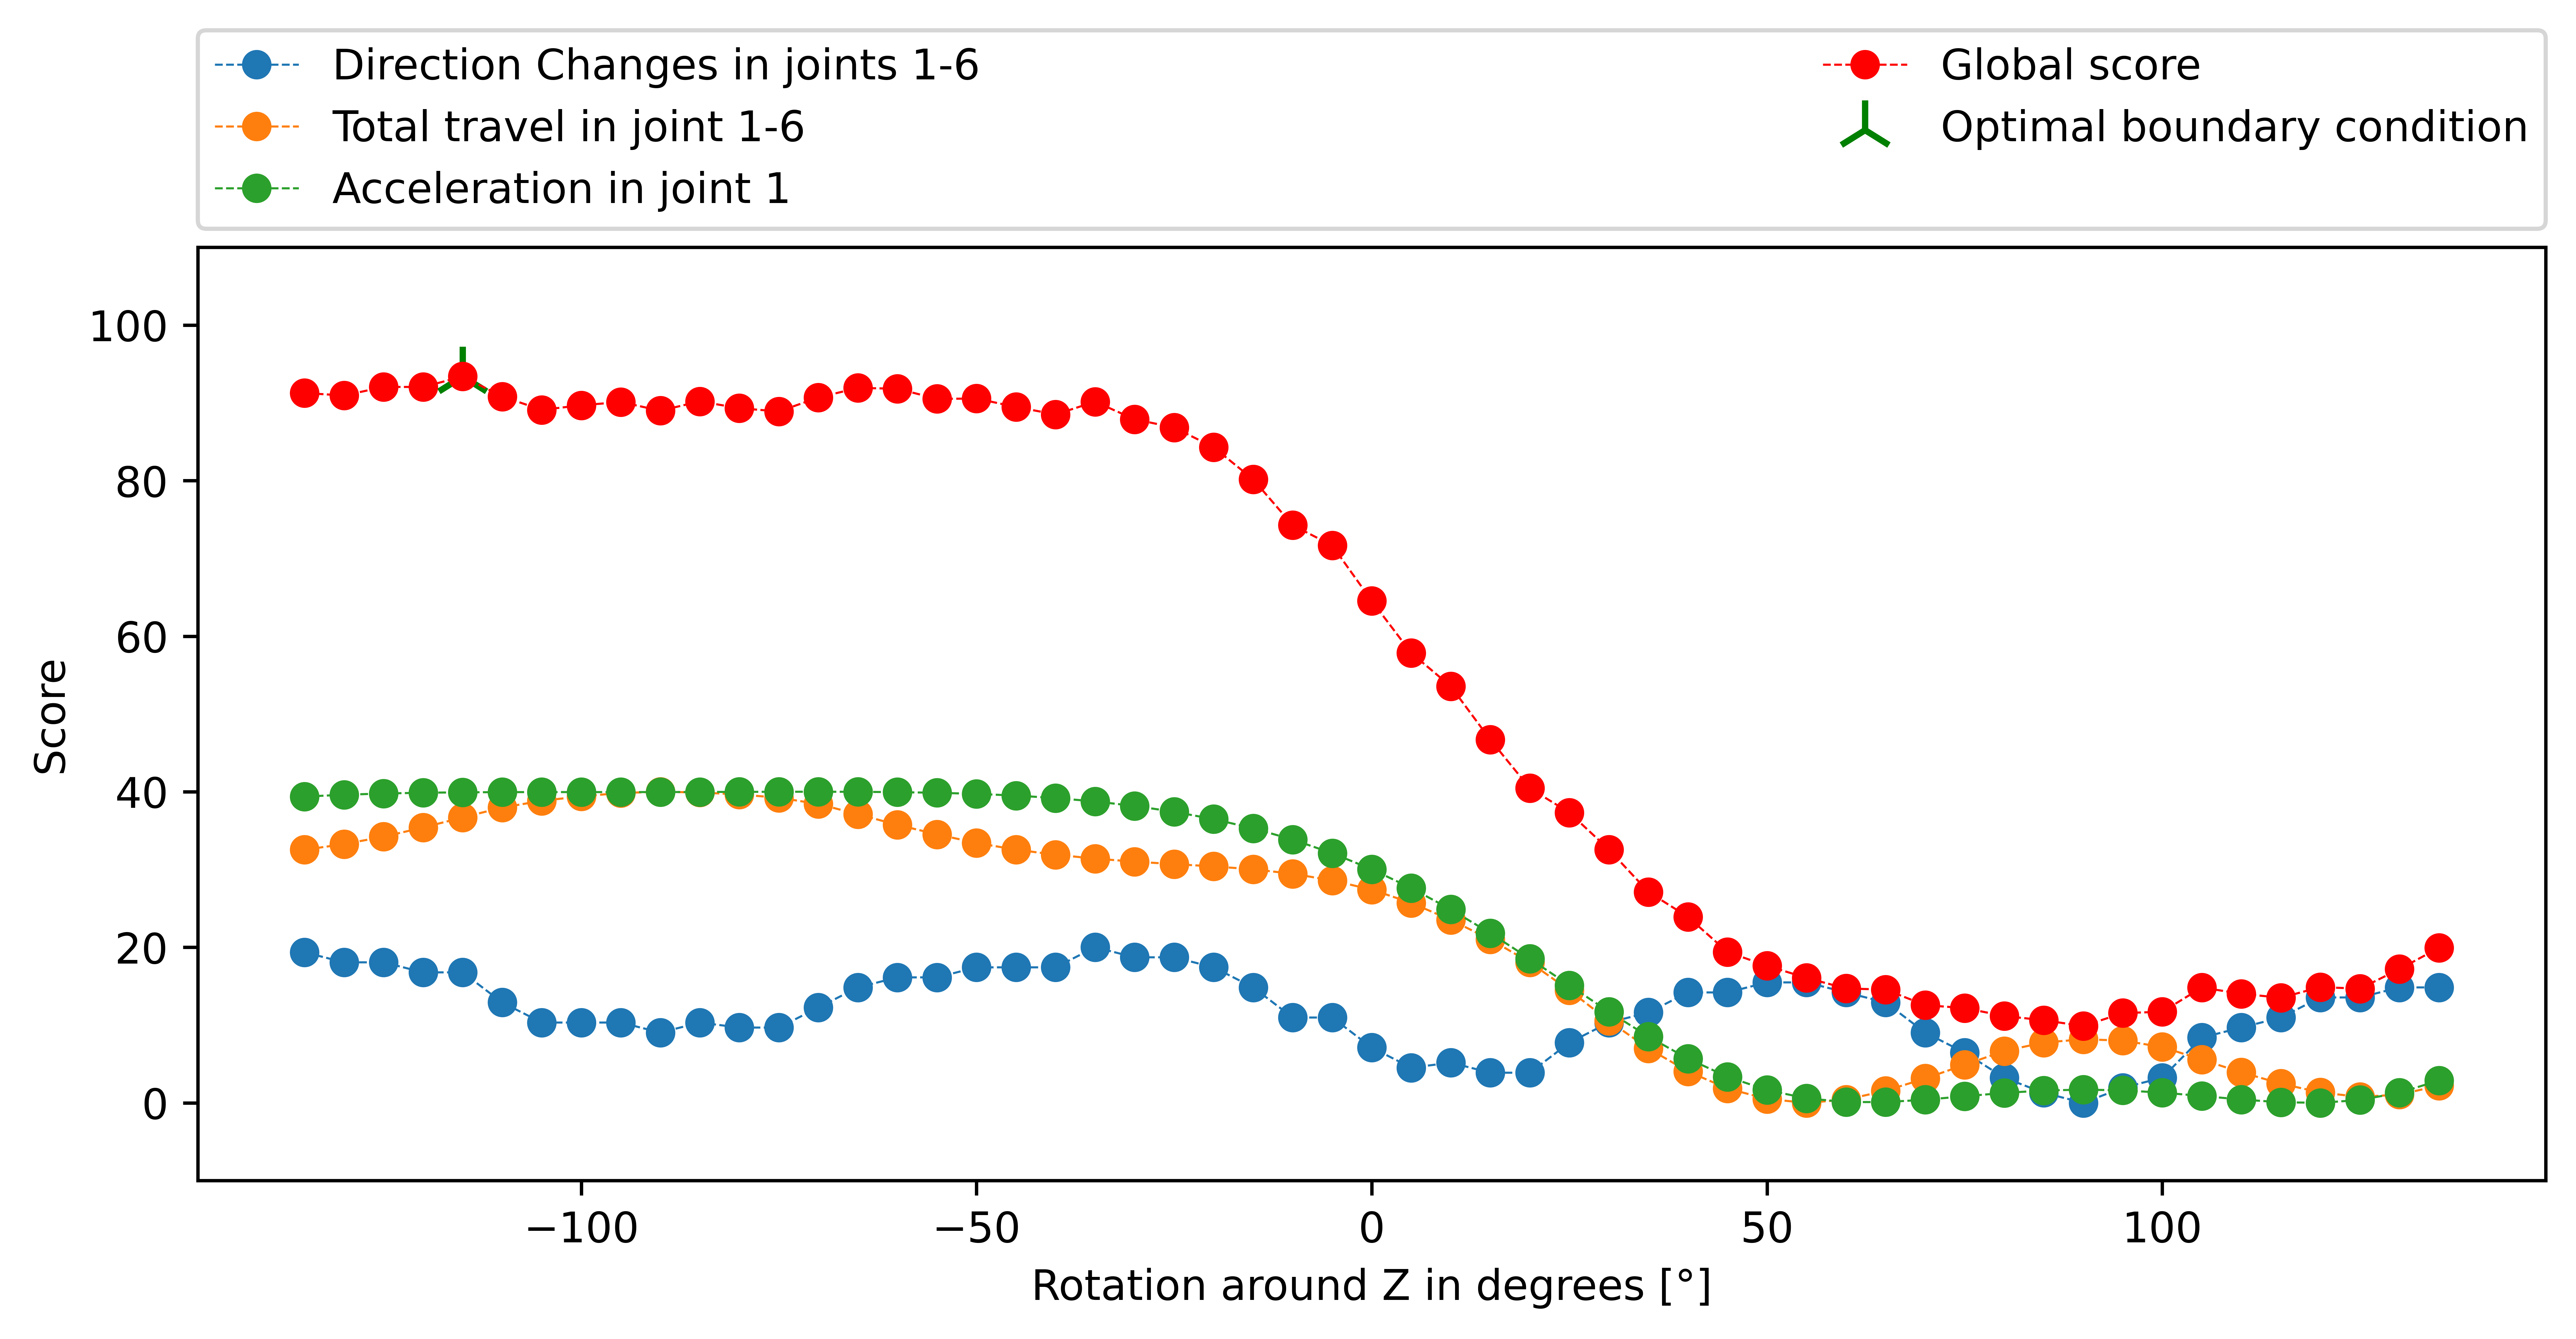
\includegraphics[width=1\textwidth]{figures/best_c_2_combi.png}}
\caption{Global and local scores in toolpath 2 depending on the rotation around Z}
\label{TP2_combi}
\end{figure}
\begin{figure}[H]
\centerline{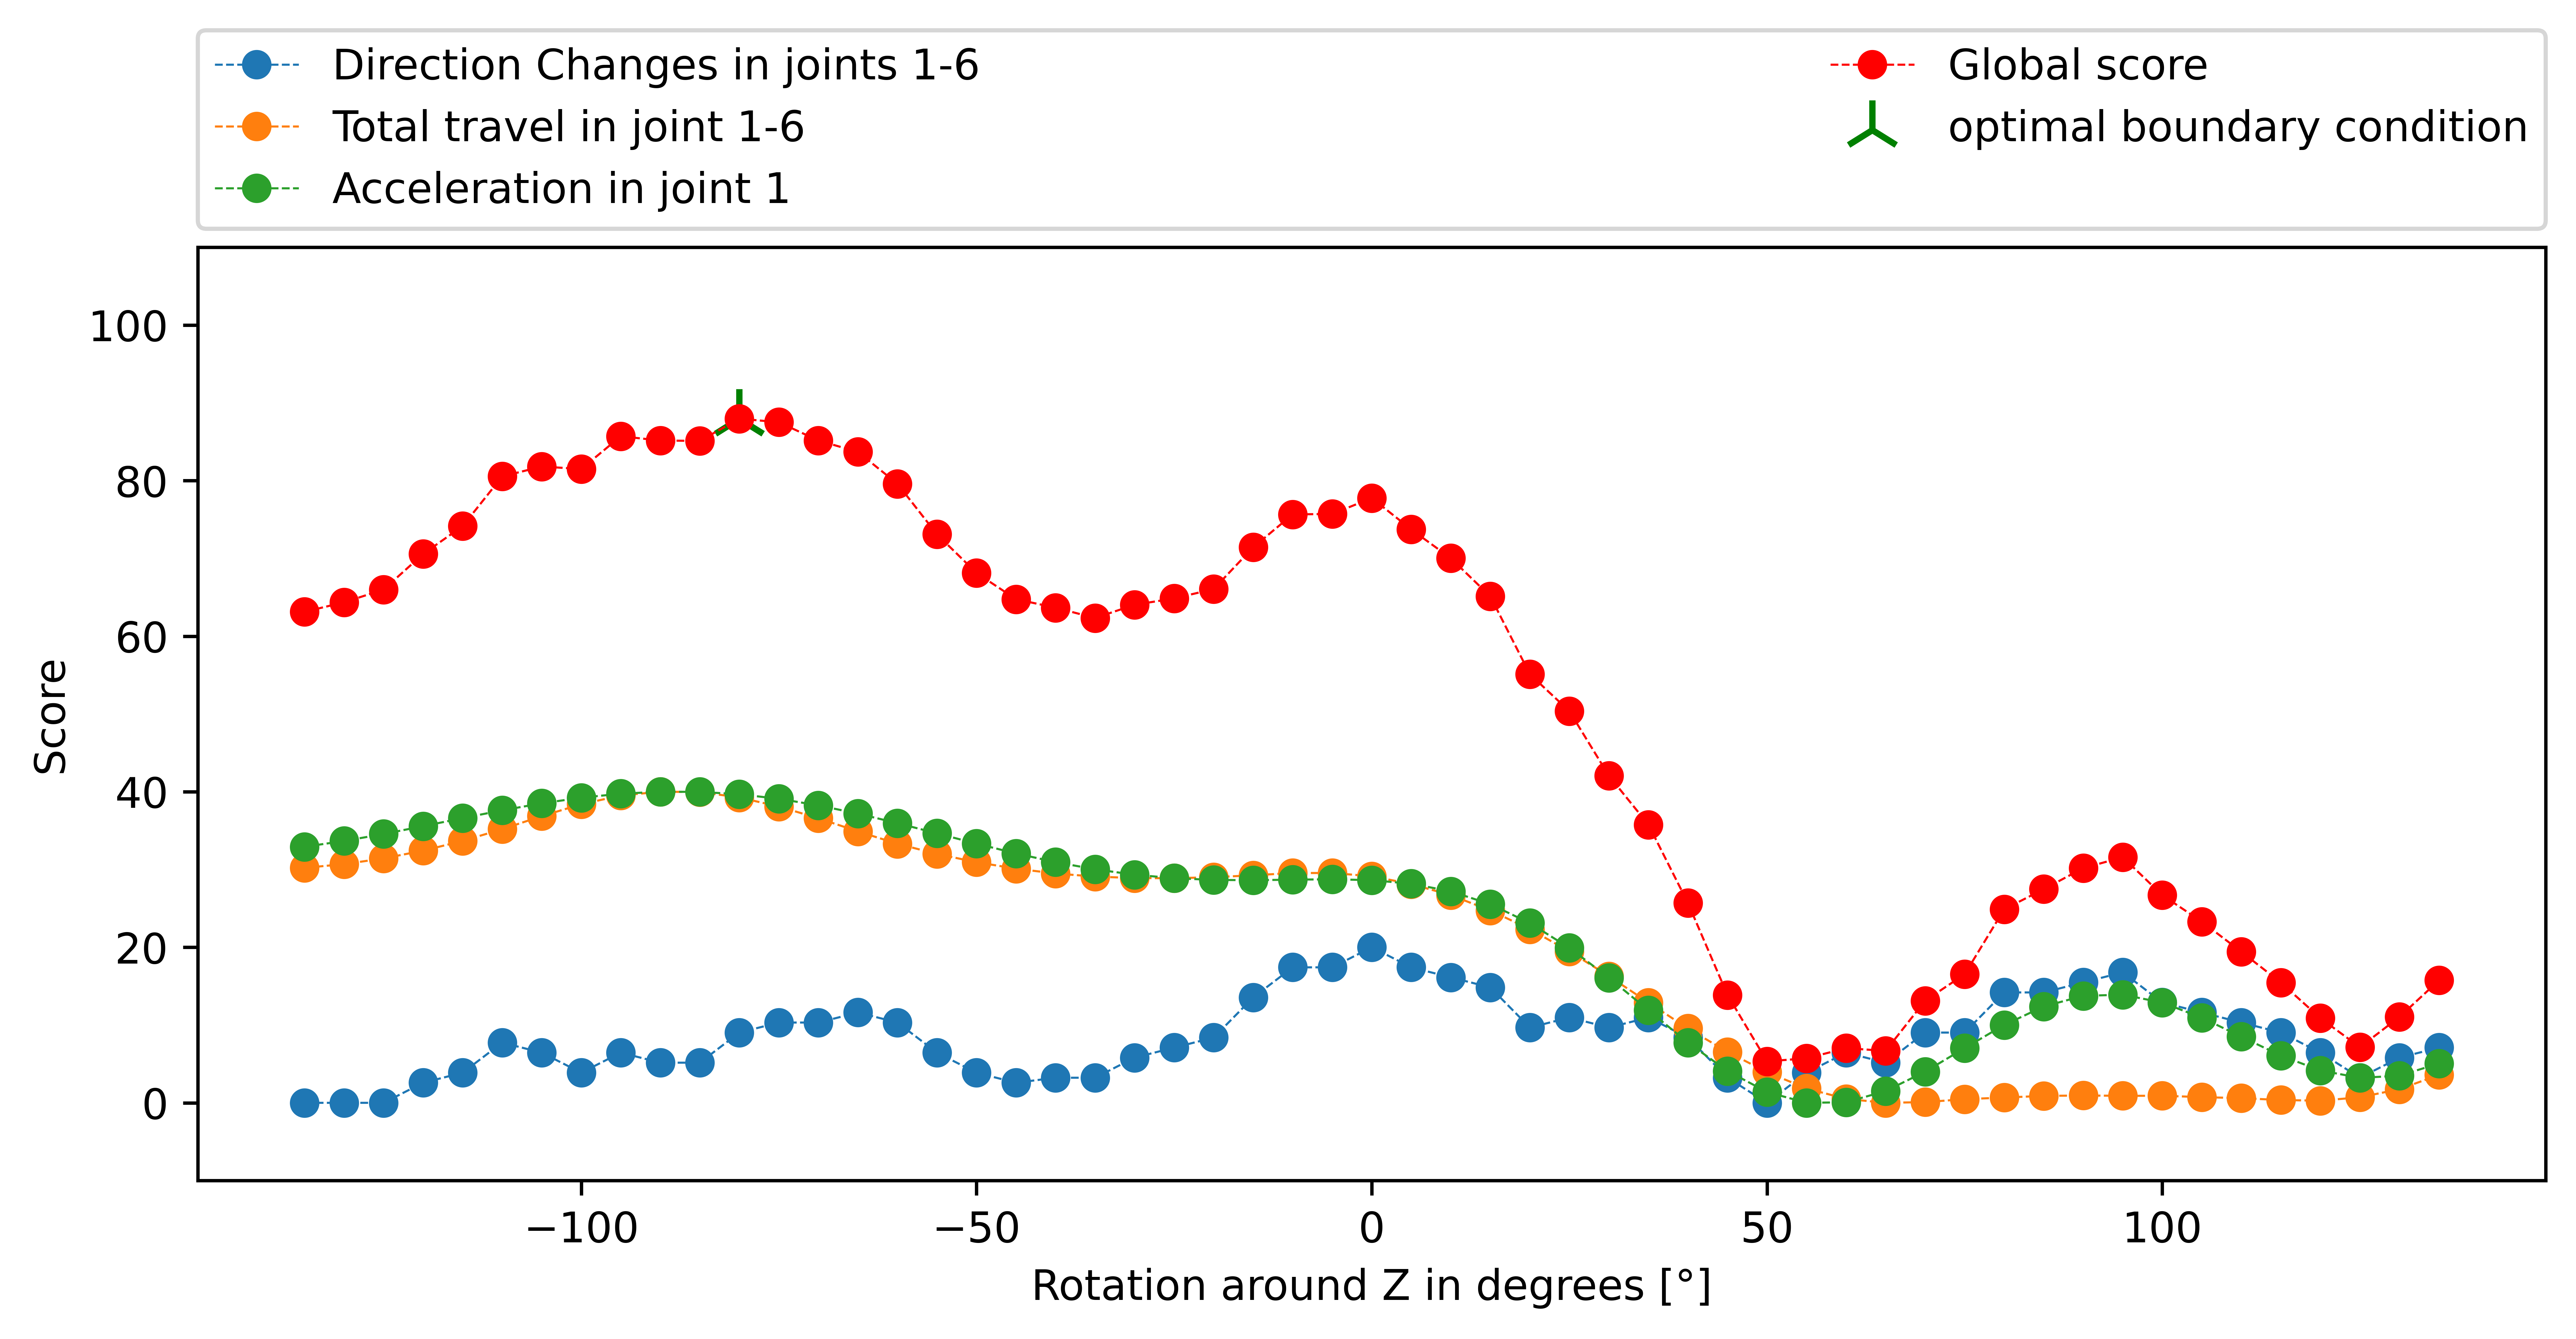
\includegraphics[width=1\textwidth]{figures/best_c_3_combi.png}}
\caption{Global and local scores in toolpath 3 depending on the rotation around Z}
\label{TP3_combi}
\end{figure}

It is noteworthy that even though all toolpaths have significantly different characteristics, all global scores show a similar trend. High global scores are achieved by setting the rotation to less than 0°, while low scores are achieved by setting the rotation to higher than 30°. Additionally, it is important to mention that when a local score reaches its maximum value, it does not imply that the corresponding process variables, such as the number of direction changes, become zero. Instead, it signifies that the number of direction changes is at its lowest compared to all other analyzed options.\newline
Based on this result, it is reasonable to conclude that correctly setting the redundant \acrshort{DoF}s can significantly improve the manufacturing process.
\newpage
\subsection{Validation on a Production Grade toolpath}\label{RG}
In addition to the three simulated toolpaths, a real toolpath used for \acrshort{WAAM} is now being used for validation. The toolpath has an organic structure that requires tilting of the rotary-tilt table to ensure that the material deposition process occurs in the direction of gravity. Thus, the position of the rotary-tilt table is not horizontal during the process. The redundant \acrshort{DoF} remains the rotation around the Z-axis of the tool, as before. Figure \ref{rav} provides a visual representation of the analyzed toolpath. It consists of 28,000 coordinates and is modeled to be traversed in 2,800 seconds.

\begin{figure}[H]
	\centerline{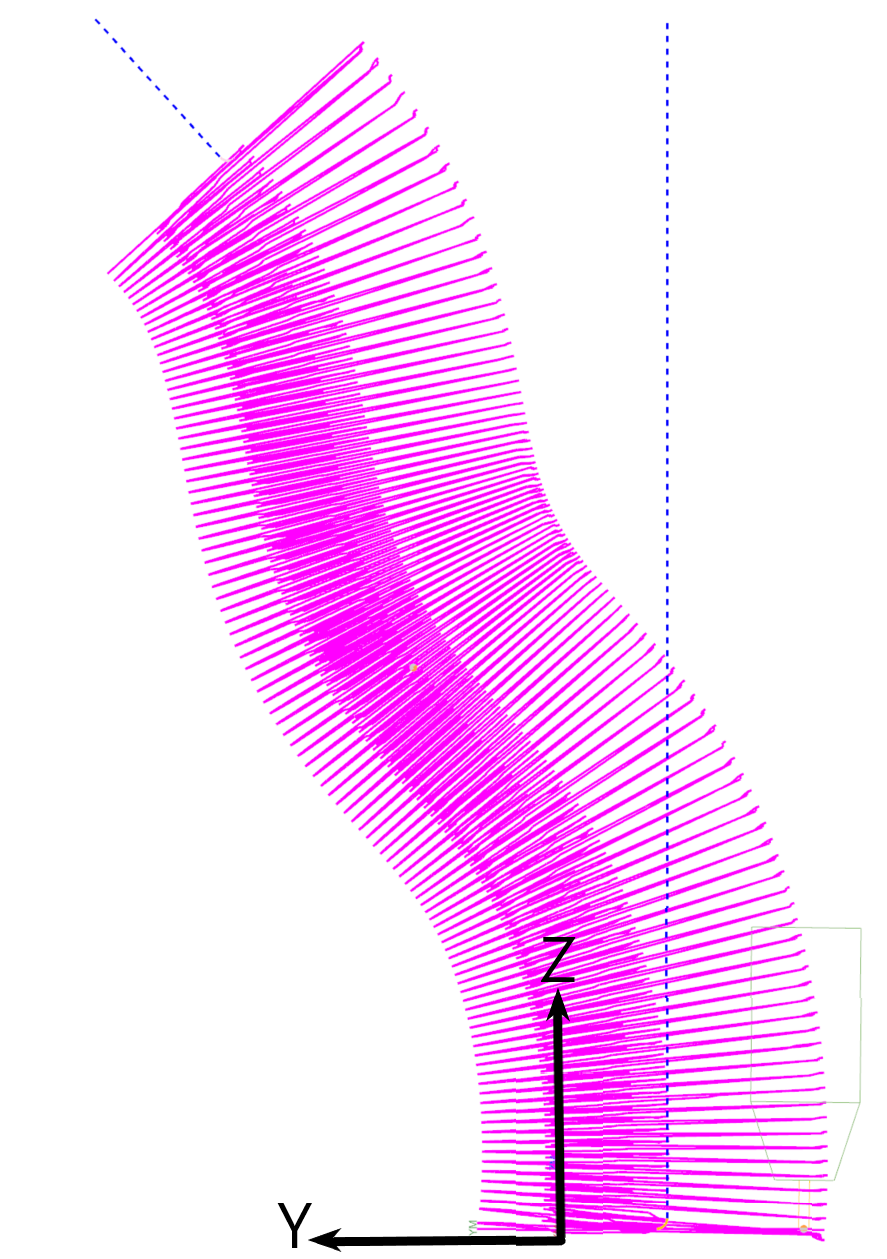
\includegraphics[width=0.3\textwidth]{figures/raven.png}}
	\caption{Organic toolpath \cite{Reisch.2023}}
	\label{rav}
\end{figure}

The process variables for the analysis of this toolpath are defined in Table \ref{ravenparams}. In this example, the direction changes in joints 1, 2, and 3 are all individually weighted with a factor of 0.2. The last two variables are the velocity in joint 5 and the total travel in joint 6. These variables are also weighted with an importance factor of 0.2. To obtain a scalar value for the velocity, all elements of the time-series are squared and summed up. 

\begin{table}[H]
	\centering
	\begin{tabular}{||l|l||}
		Process variables& Importance factors \\
		\hline
		\hline
		\hline
		Direction changes in joint 1	&		0.2 \\
		Direction changes in joint 2	&		0.2 \\
		Direction changes in joint 3	&		0.2 \\
		Velocity in joint 5	&		0.2 \\
		Total travel in joint 6	&		0.2 \\
		\hline
		\hline
	\end{tabular}
	
	\caption{Selected process variables and their importance factors for the organic toolpath}
	\label{ravenparams}
\end{table}

The redundant \acrshort{DoF} is once again analyzed in 5° increments, starting from -135° and ending at 135°. The resulting local scores are shown in Figure \ref{LS4}. It is evident that the velocity in joint 5 and the total travel in joint 6 exhibit a smooth oscillating behavior. The direction changes in joint 1 remain constant for all analyzed settings of the redundant \acrshort{DoF}. Therefore, the local score is set to 0 and is not further used in the calculation of the global score. The direction changes in joint 2 and 3 show a slight oscillation and exhibit a non-smooth progression towards the end and beginning of the analyzed range.

\begin{figure}[H]
	\centerline{\includegraphics[width=1\textwidth]{figures/LocalScores_4.png}}
	\caption{Global score for toolpath 1}
	\label{LS4}
\end{figure}

Figure \ref{GS4} illustrates the combined local scores in the form of the global score. The highest global score is 75.5, which is achieved by setting the C-axis to -15°. Notably, in the range from -70° to 40°, a very smooth curve is observed. This smooth progression of the global score serves as a strong indicator that an optimization algorithm will easily find an optimum setting for the redundant \acrshort{DoF}.

\begin{figure}[H]
	\centerline{\includegraphics[width=1\textwidth]{figures/best_c_4.png}}
	\caption{Global score for production toolpath}
	\label{GS4}
\end{figure}


\newpage

\subsection{Toolpath Evaluation With two Redundant DoF}\label{2RDOF}

To introduce an additional redundant \acrshort{DoF}, a rotary-tilt table is simulated. Currently, only the tilting aspect is being analyzed. All coordinates of the toolpath can be rotated by a specified degree around the X-axis of the toolpath coordinate system. Figure \ref{TP3_0} depicts toolpath 3 with no rotation around the X-axis, while Figure \ref{TP3_25} illustrates a rotation of +25 degrees.

\begin{figure}[H]% [H] is so declass\'e!
	\centering
	\begin{minipage}{0.5\textwidth}
		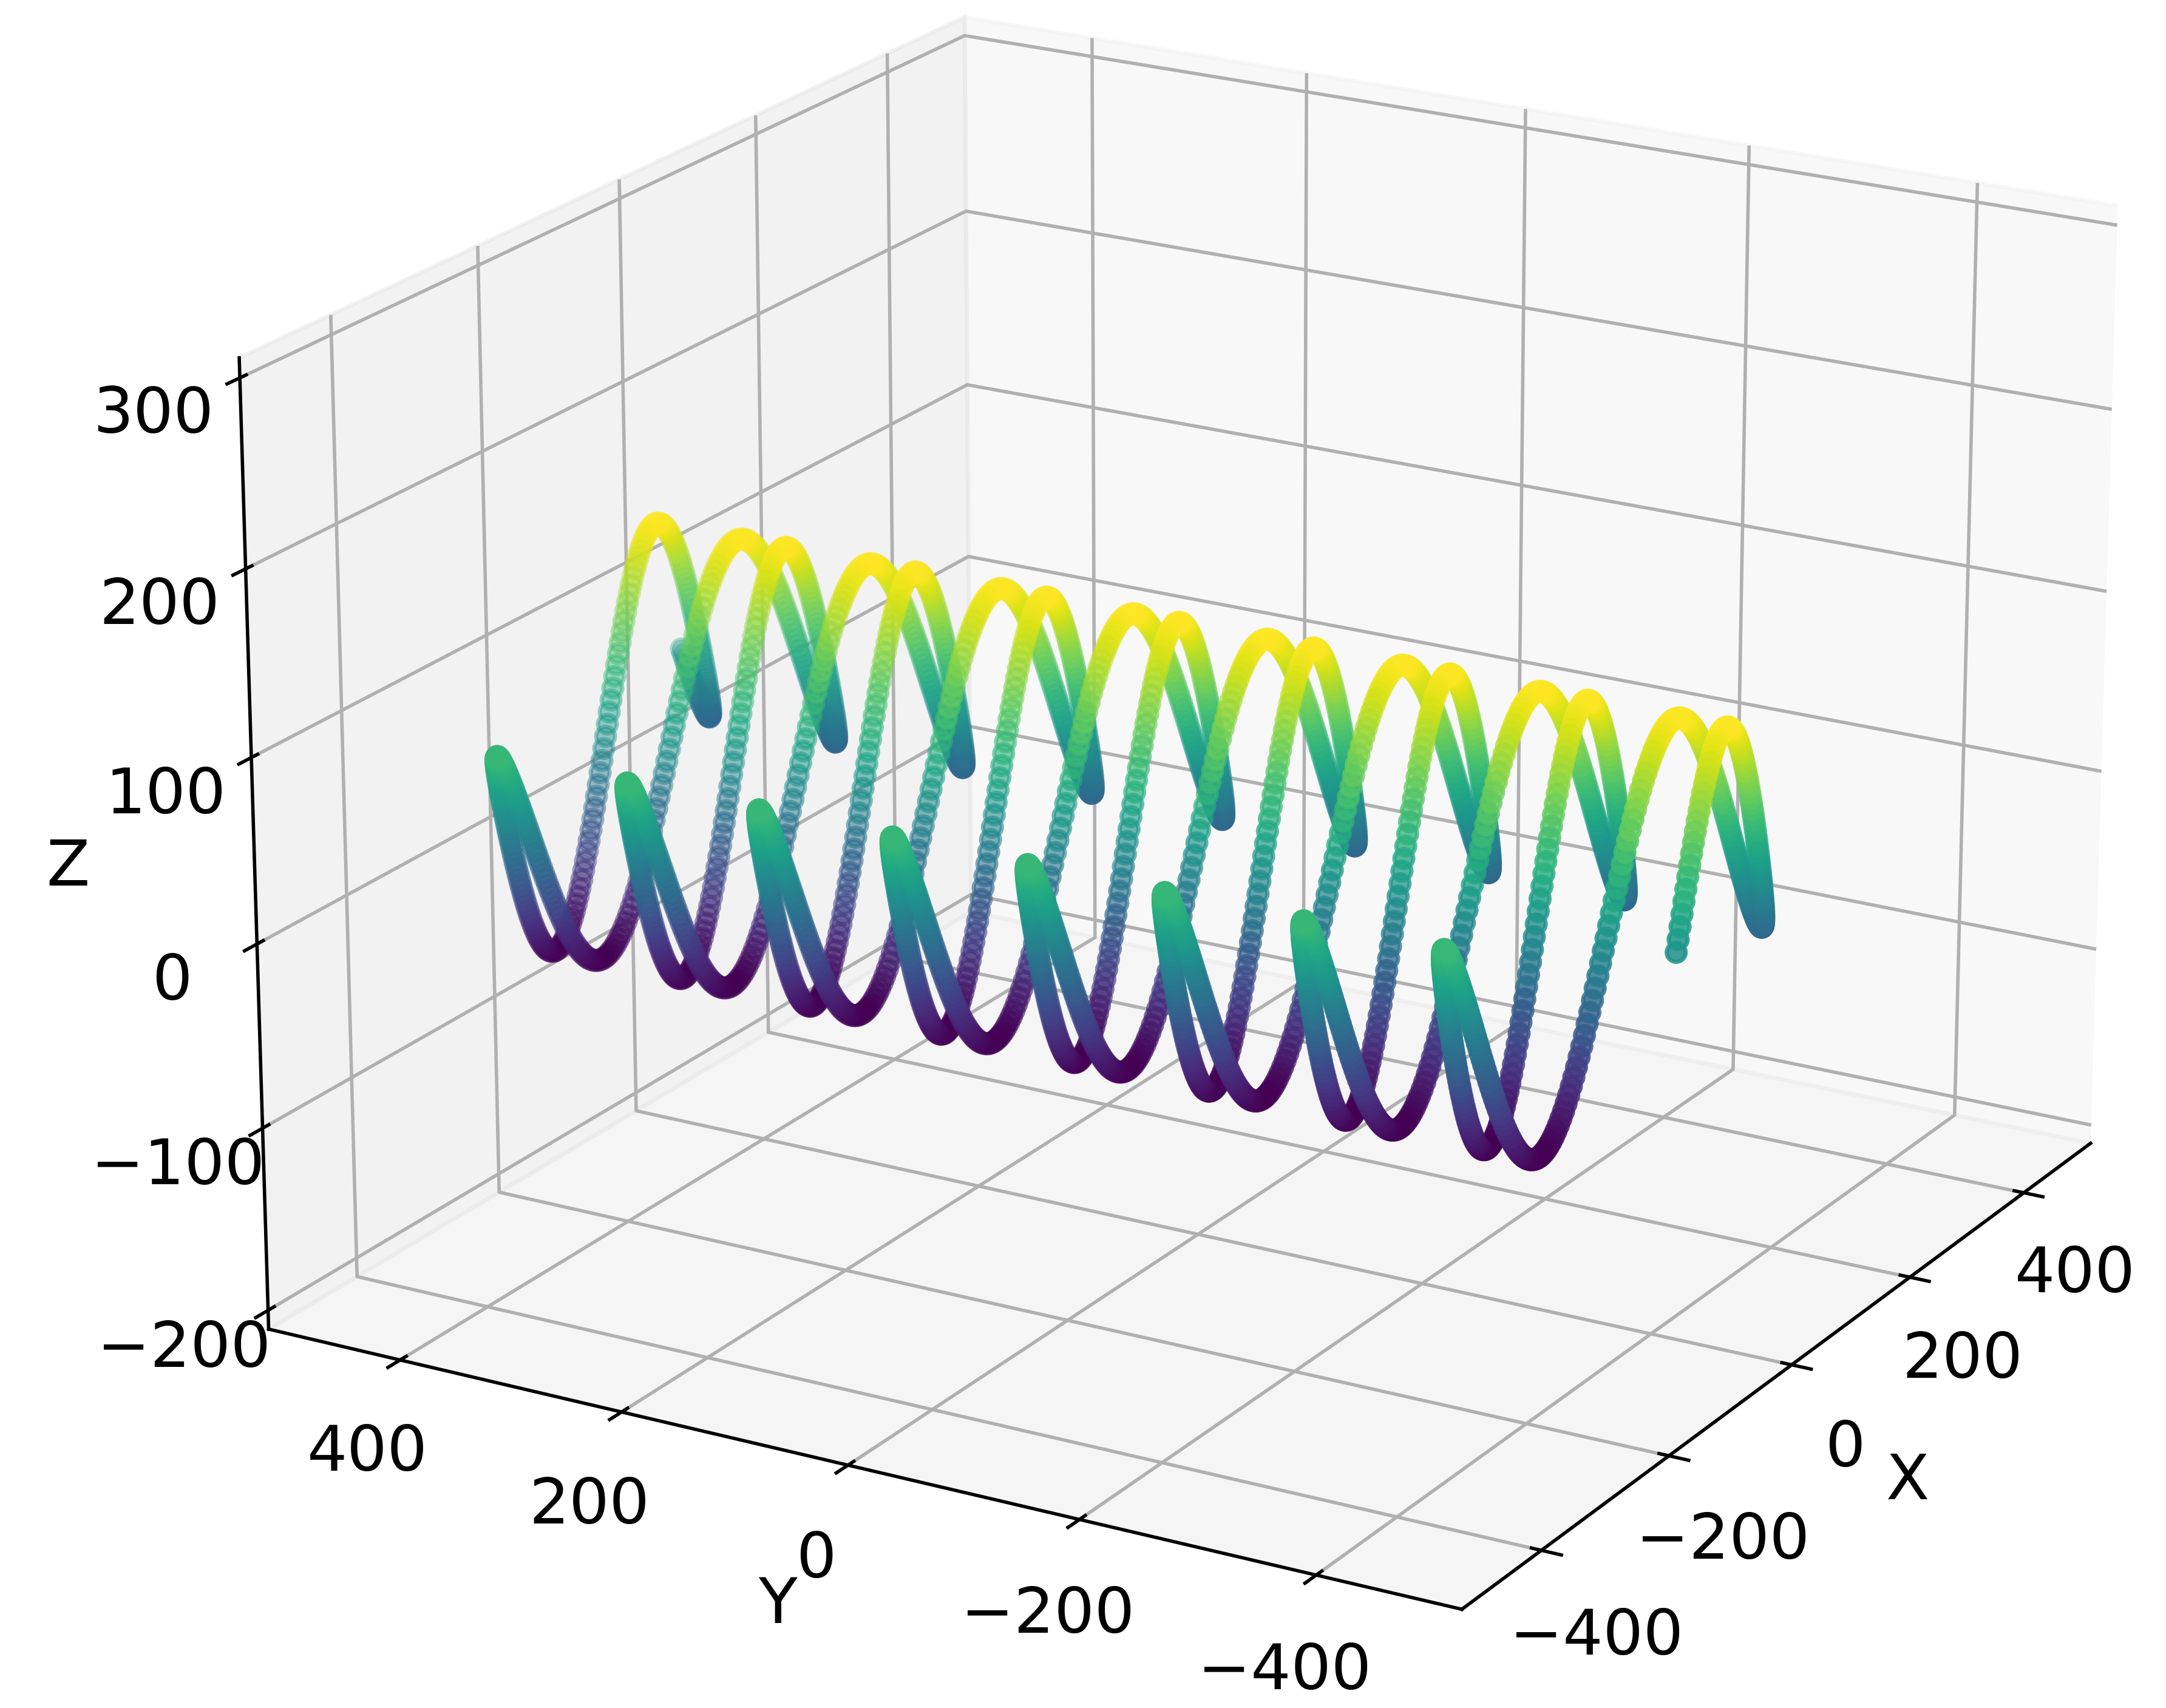
\includegraphics[width=\textwidth]{figures/path3_kipp_0_comparison.png}
		\caption{Toolpath 3 with no rotation\newline around the X-axis}
		\label{TP3_0}
	\end{minipage}\hfill
	\begin{minipage}{0.5\textwidth}
		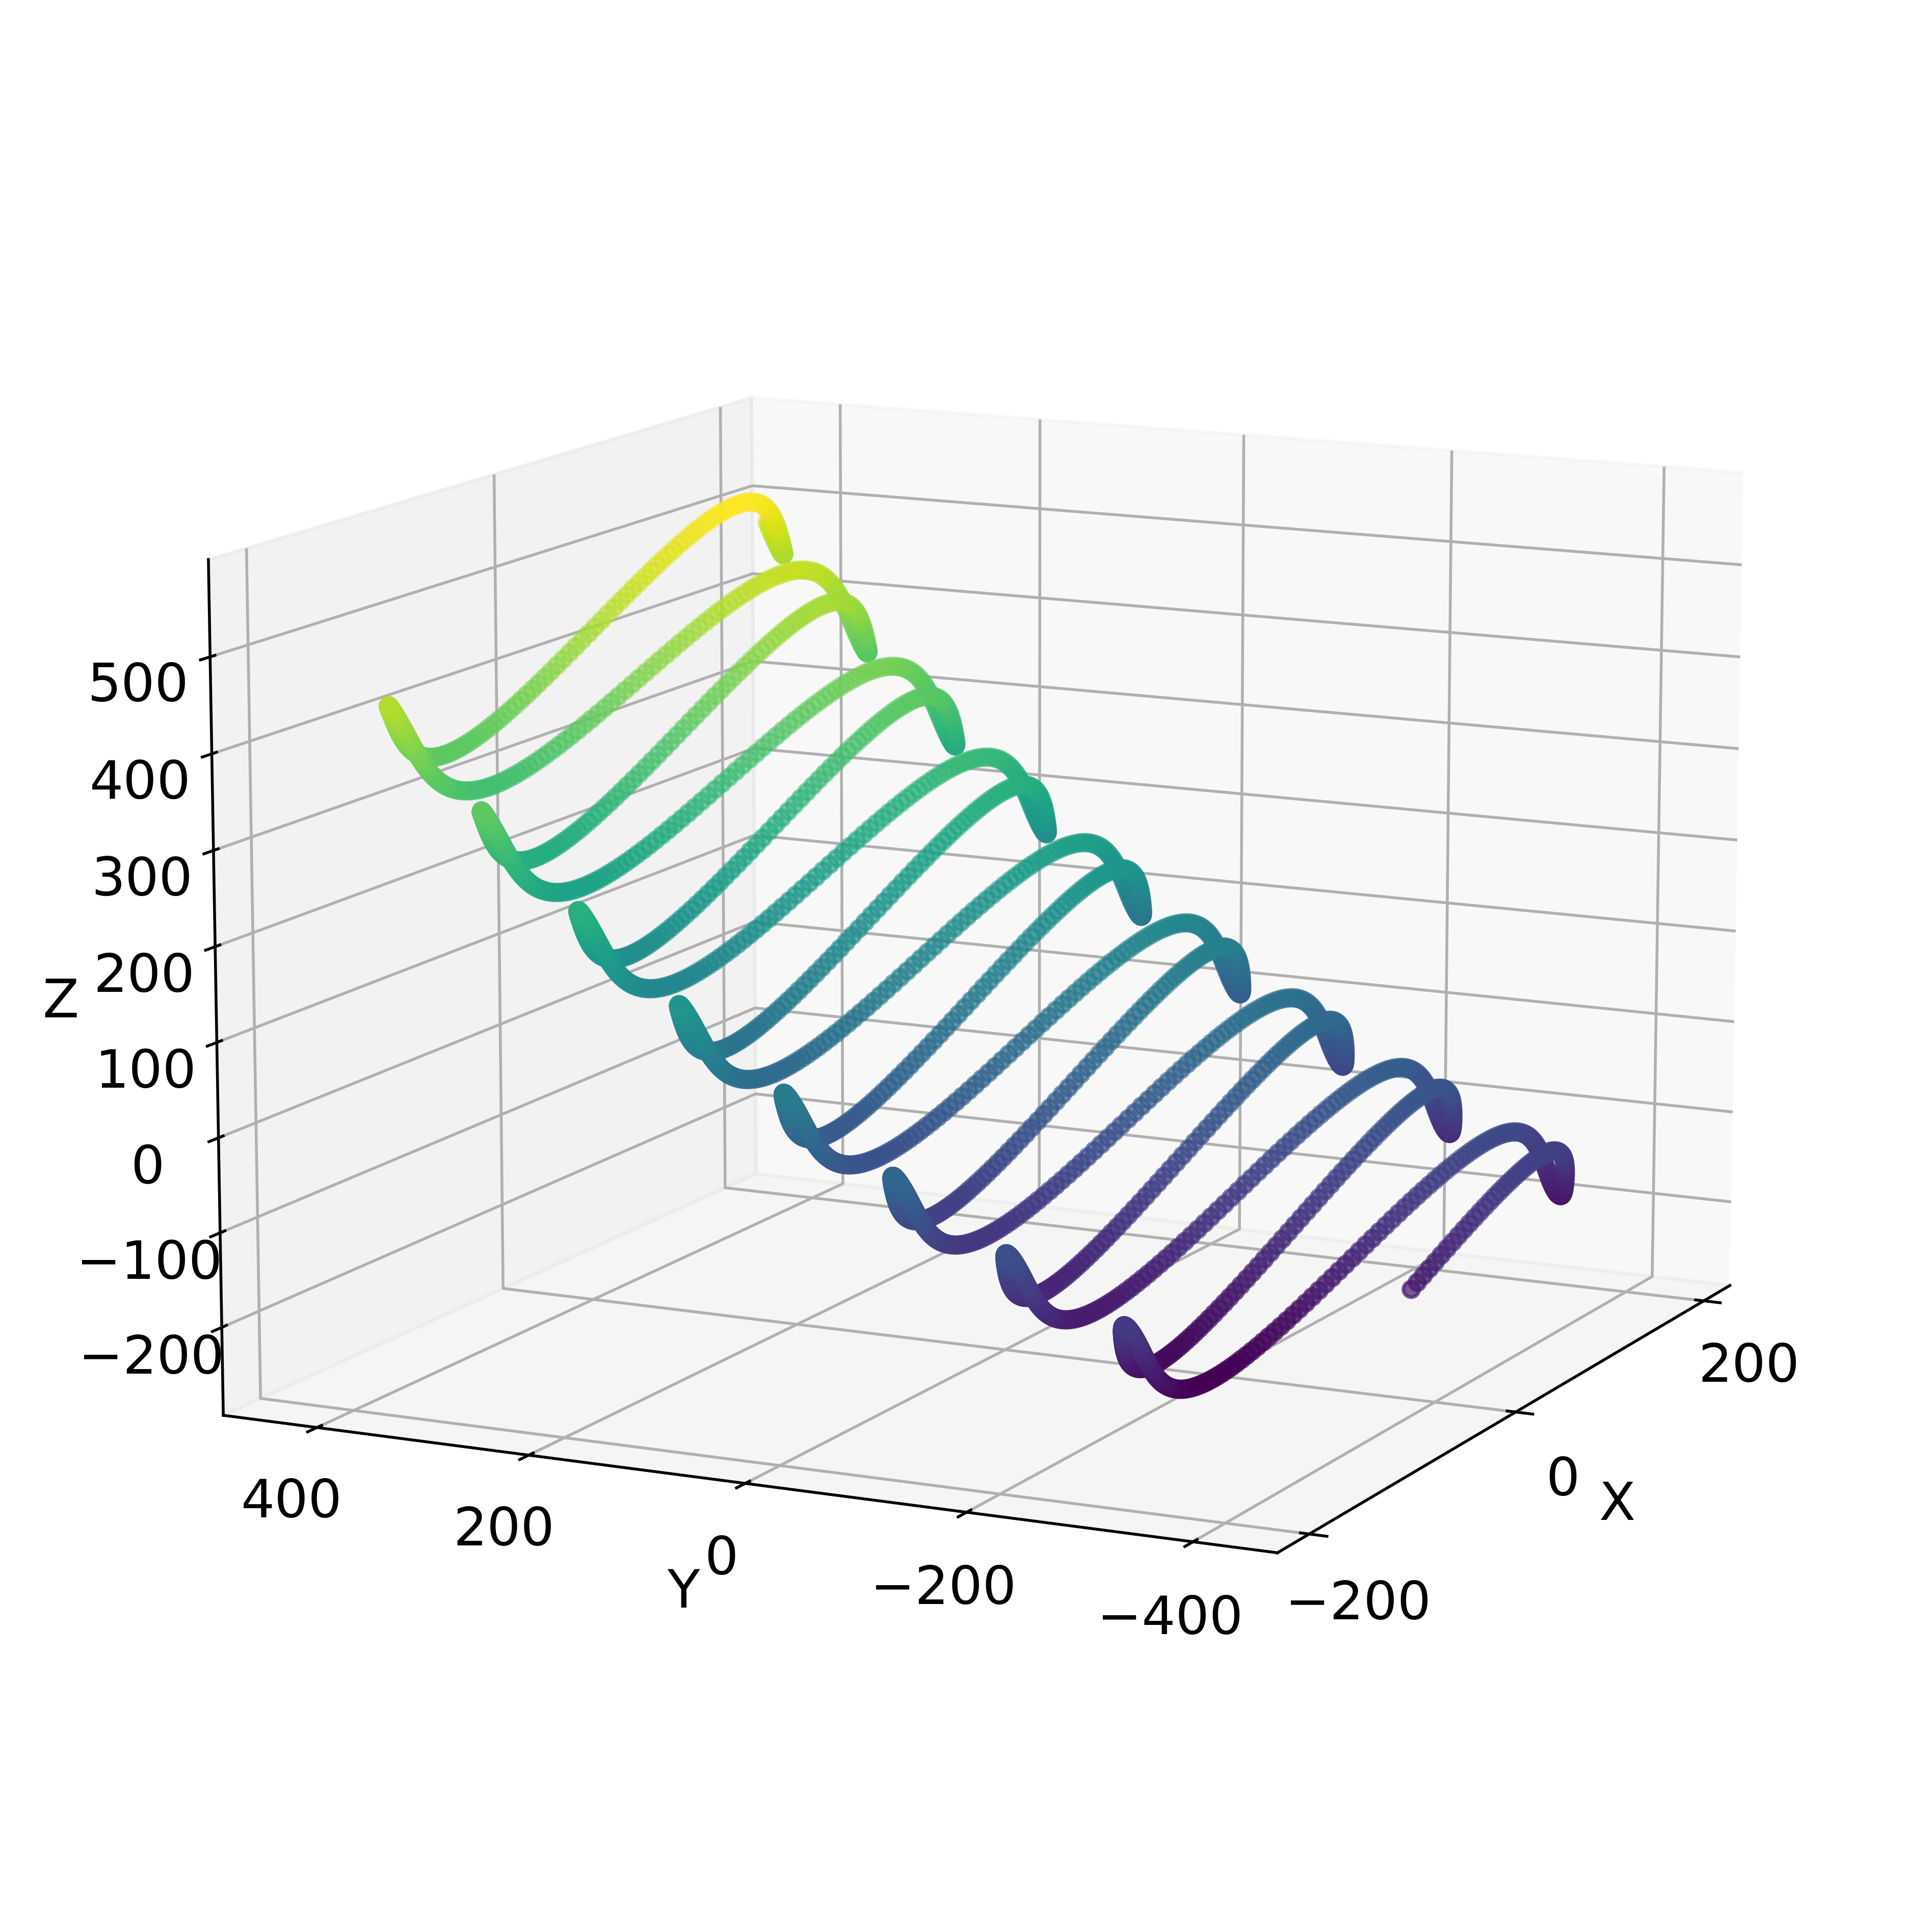
\includegraphics[width=\textwidth]{figures/path3_kipp_25_comparison.png}
		\caption{Toolpath 3 with a rotation\newline of 25 degrees around the X-axis}
		\label{TP3_25}
	\end{minipage}\par
\end{figure}
 

Similar to the previous analysis, the same steps need to be followed. The newly selected process variables are presented in Table \ref{PP_2}. The direction changes of the tilting joints (2+3+5) are combined and treated as one process variable, weighted with a factor of 0.3. Direction changes in joint 1 and acceleration in joint 4 are considered as individual variables, both individually weighted with 0.25. The final variable is the velocity in joint 6, weighted with 0.2.

\begin{table}[H]
	\centering
	\begin{tabular}{||l|l||}
		Process variables & Importance factors \\
		\hline
		\hline
		\hline
		Direction changes in joints 2+3+5	&		0.3 \\
		Direction changes in joints 1	& 	0.25 \\
		Acceleration in joint 4	& 		0.25\\
		Velocity in joint 6	& 		0.2\\
		\hline
		\hline
	\end{tabular}
	
	\caption{Selected process variables and their importance factors for 2 redundant DoF}
	\label{PP_2}
\end{table}


Figure \ref{TP3_25_robot} displays the robot and its orientation while following the tilted toolpath 3. It is crucial to note that since the toolpath is defined in 5 \acrshort{DoF}s in its own frame, the frame of the \acrshort{TCP} must also tilt by the same degree as the table. The two redundant \acrshort{DoF}s in this case are the rotation around the Z-axis in the frame of the tilted toolpath and the tilting of the toolpath itself. This introduces an additional dimension, as now two parameters can be adapted for optimization.


\begin{figure}[H]
	\centerline{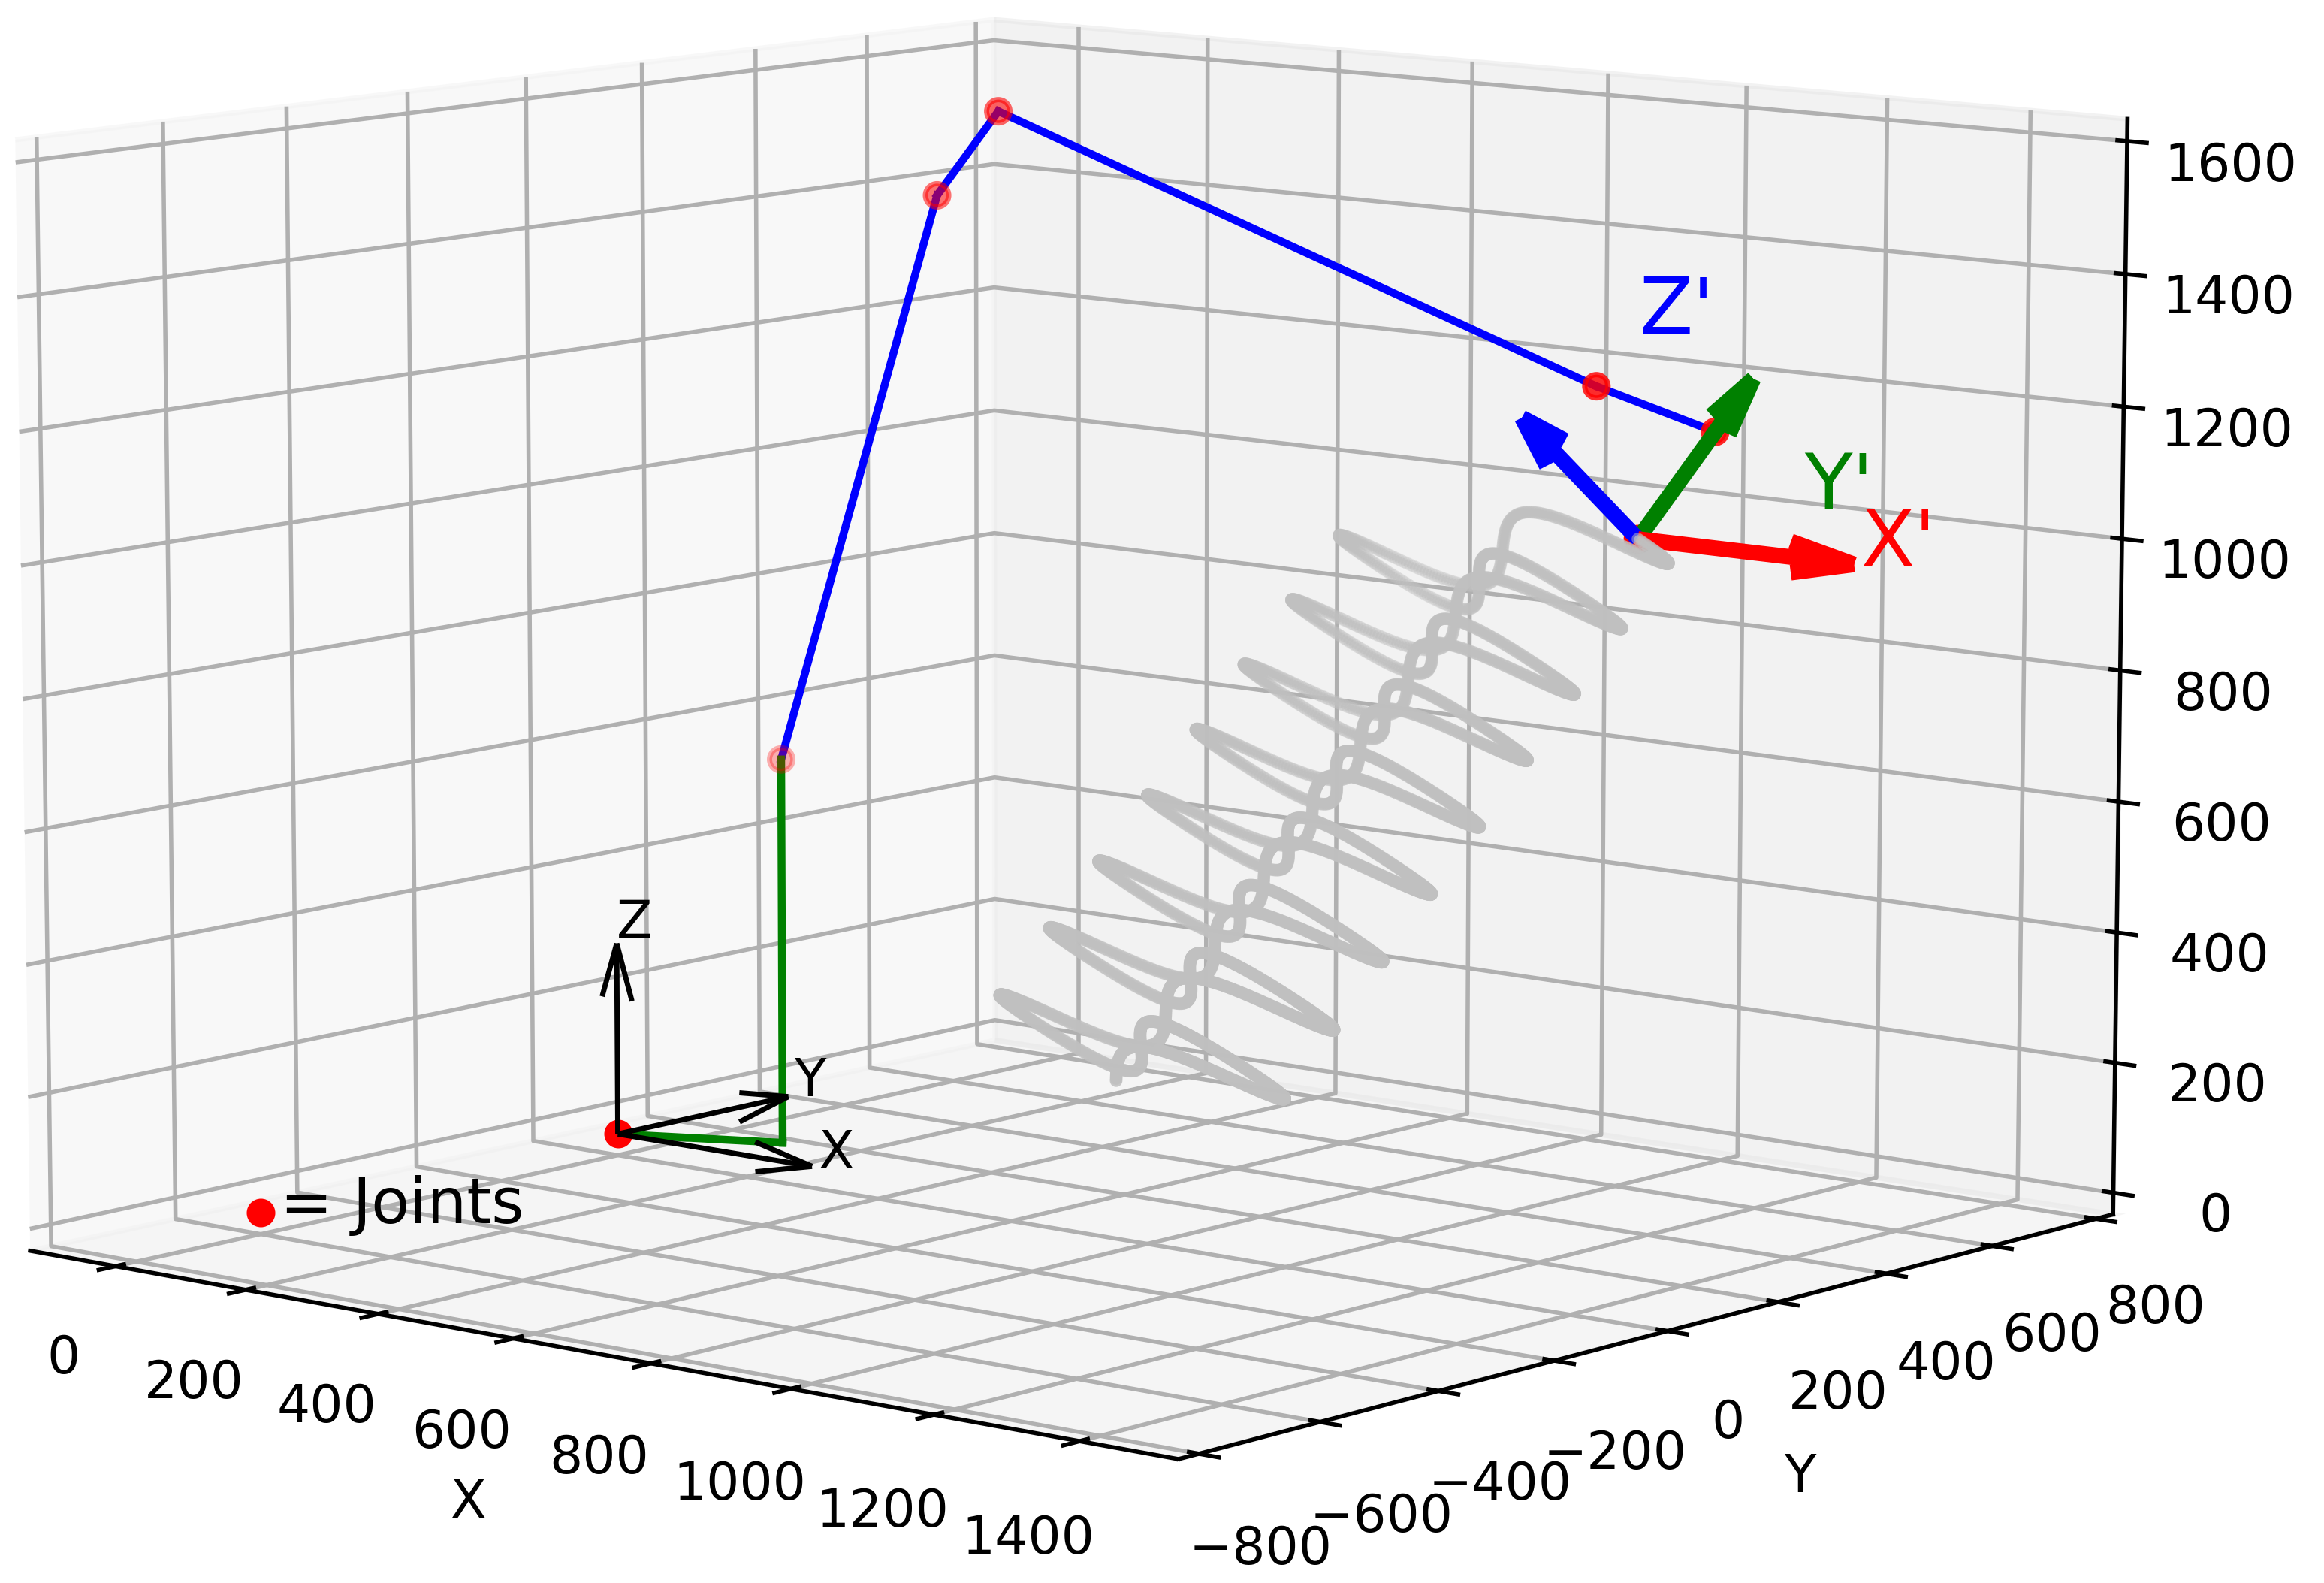
\includegraphics[width=0.9\textwidth]{figures/robotANDpath3_45.png}}
	\caption{Robot following the tilted toolpath 3}
	\label{TP3_25_robot}
\end{figure}

The range of possible tilt positions ranges from -45° to 45° in 2-degree increments. For every combination of tilt and rotation, the joint angles are generated using inverse kinematics. To speed up the computation, only every third coordinate is utilized in the inverse kinematic algorithm. This reduces the toolpath by 2000 points and speeds up calculation time. On average, it now takes only 10 seconds to calculate the joint positions. A total of 2530 individual combinations are analyzed.

The extracted process variables are again multiplied by -1, as the objective is to minimize them. Afterwards, the Min-Max scaler is applied. The individual values are aggregated and presented in the form of a matrix. The values of this matrix are visualized in Figure \ref{best_2D}. The maximum achievable score from all possible combinations is 70.4, visualized by the red cross. This score was attained by setting the table tilt to -5° and the rotation around the Z-axis of the tool to +35°. The resulting hyperplane exhibits two distinct local maxima. The entire surface displays a smooth curvature, although it appears less smooth in the range from -20° to 45°.


\begin{figure}[H]
	\centerline{\includegraphics[width=1\textwidth]{figures/best_2D_3.png}}
	\caption{Hyperplane representing the global score of toolpath 3}
	\label{best_2D}
\end{figure}

The same analysis is performed with toolpath 1 and toolpath 2. The resulting matrix of the global scores for each possible boundary condition combination is shown in Figure \ref{best_2D_1} and Figure \ref{best_2D_2}, respectively. The same process variables and weights (see Table \ref{PP_2}) are used for the calculations.
\newpage

\begin{figure}[H]
	\centerline{\includegraphics[width=0.7\textwidth]{figures/best_2D_1.png}}
	\caption{Hyperplane representing the global score of toolpath 1}
	\label{best_2D_1}
\end{figure}

\begin{figure}[H]
	\centerline{\includegraphics[width=0.7\textwidth]{figures/best_2D_2.png}}
	\caption{Hyperplane representing the global score of toolpath 2}
	\label{best_2D_2}
\end{figure}


\newpage
\subsection{Boundary Condition Optimization }
So far, only the analysis of different boundary conditions has been performed by exploring the entire range of possible settings for the redundant \acrshort{DoF}s. However, this approach is very time-consuming and becomes exponentially more complex with additional redundant \acrshort{DoF} and a finer step size. To address this issue and efficiently search the extensive solution space for optimal values of the redundant \acrshort{DoF}, a \acrshort{PSO} algorithm is proposed. In this algorithm, individual particles navigate the search space by adjusting their positions based on their own best position and the best position found by the entire swarm. This cooperative behavior enables the particles to explore the search space more effectively and converge towards the best solution (see Chapter \ref{OA}).

The first test is conducted using the global score matrix of toolpath 3. Initially, 20 particles are randomly placed on the plane. Each particle's score is determined by the corresponding global score at its position. By increasing the number of particles and iterations, the search space can be analyzed more comprehensively. Figure \ref{PSO_1} illustrates the randomly placed particles on the pre-calculated global score matrix of toolpath 3, considering the previously selected importance factors (see table \ref{PP_2}).

\begin{figure}[H]
	\centerline{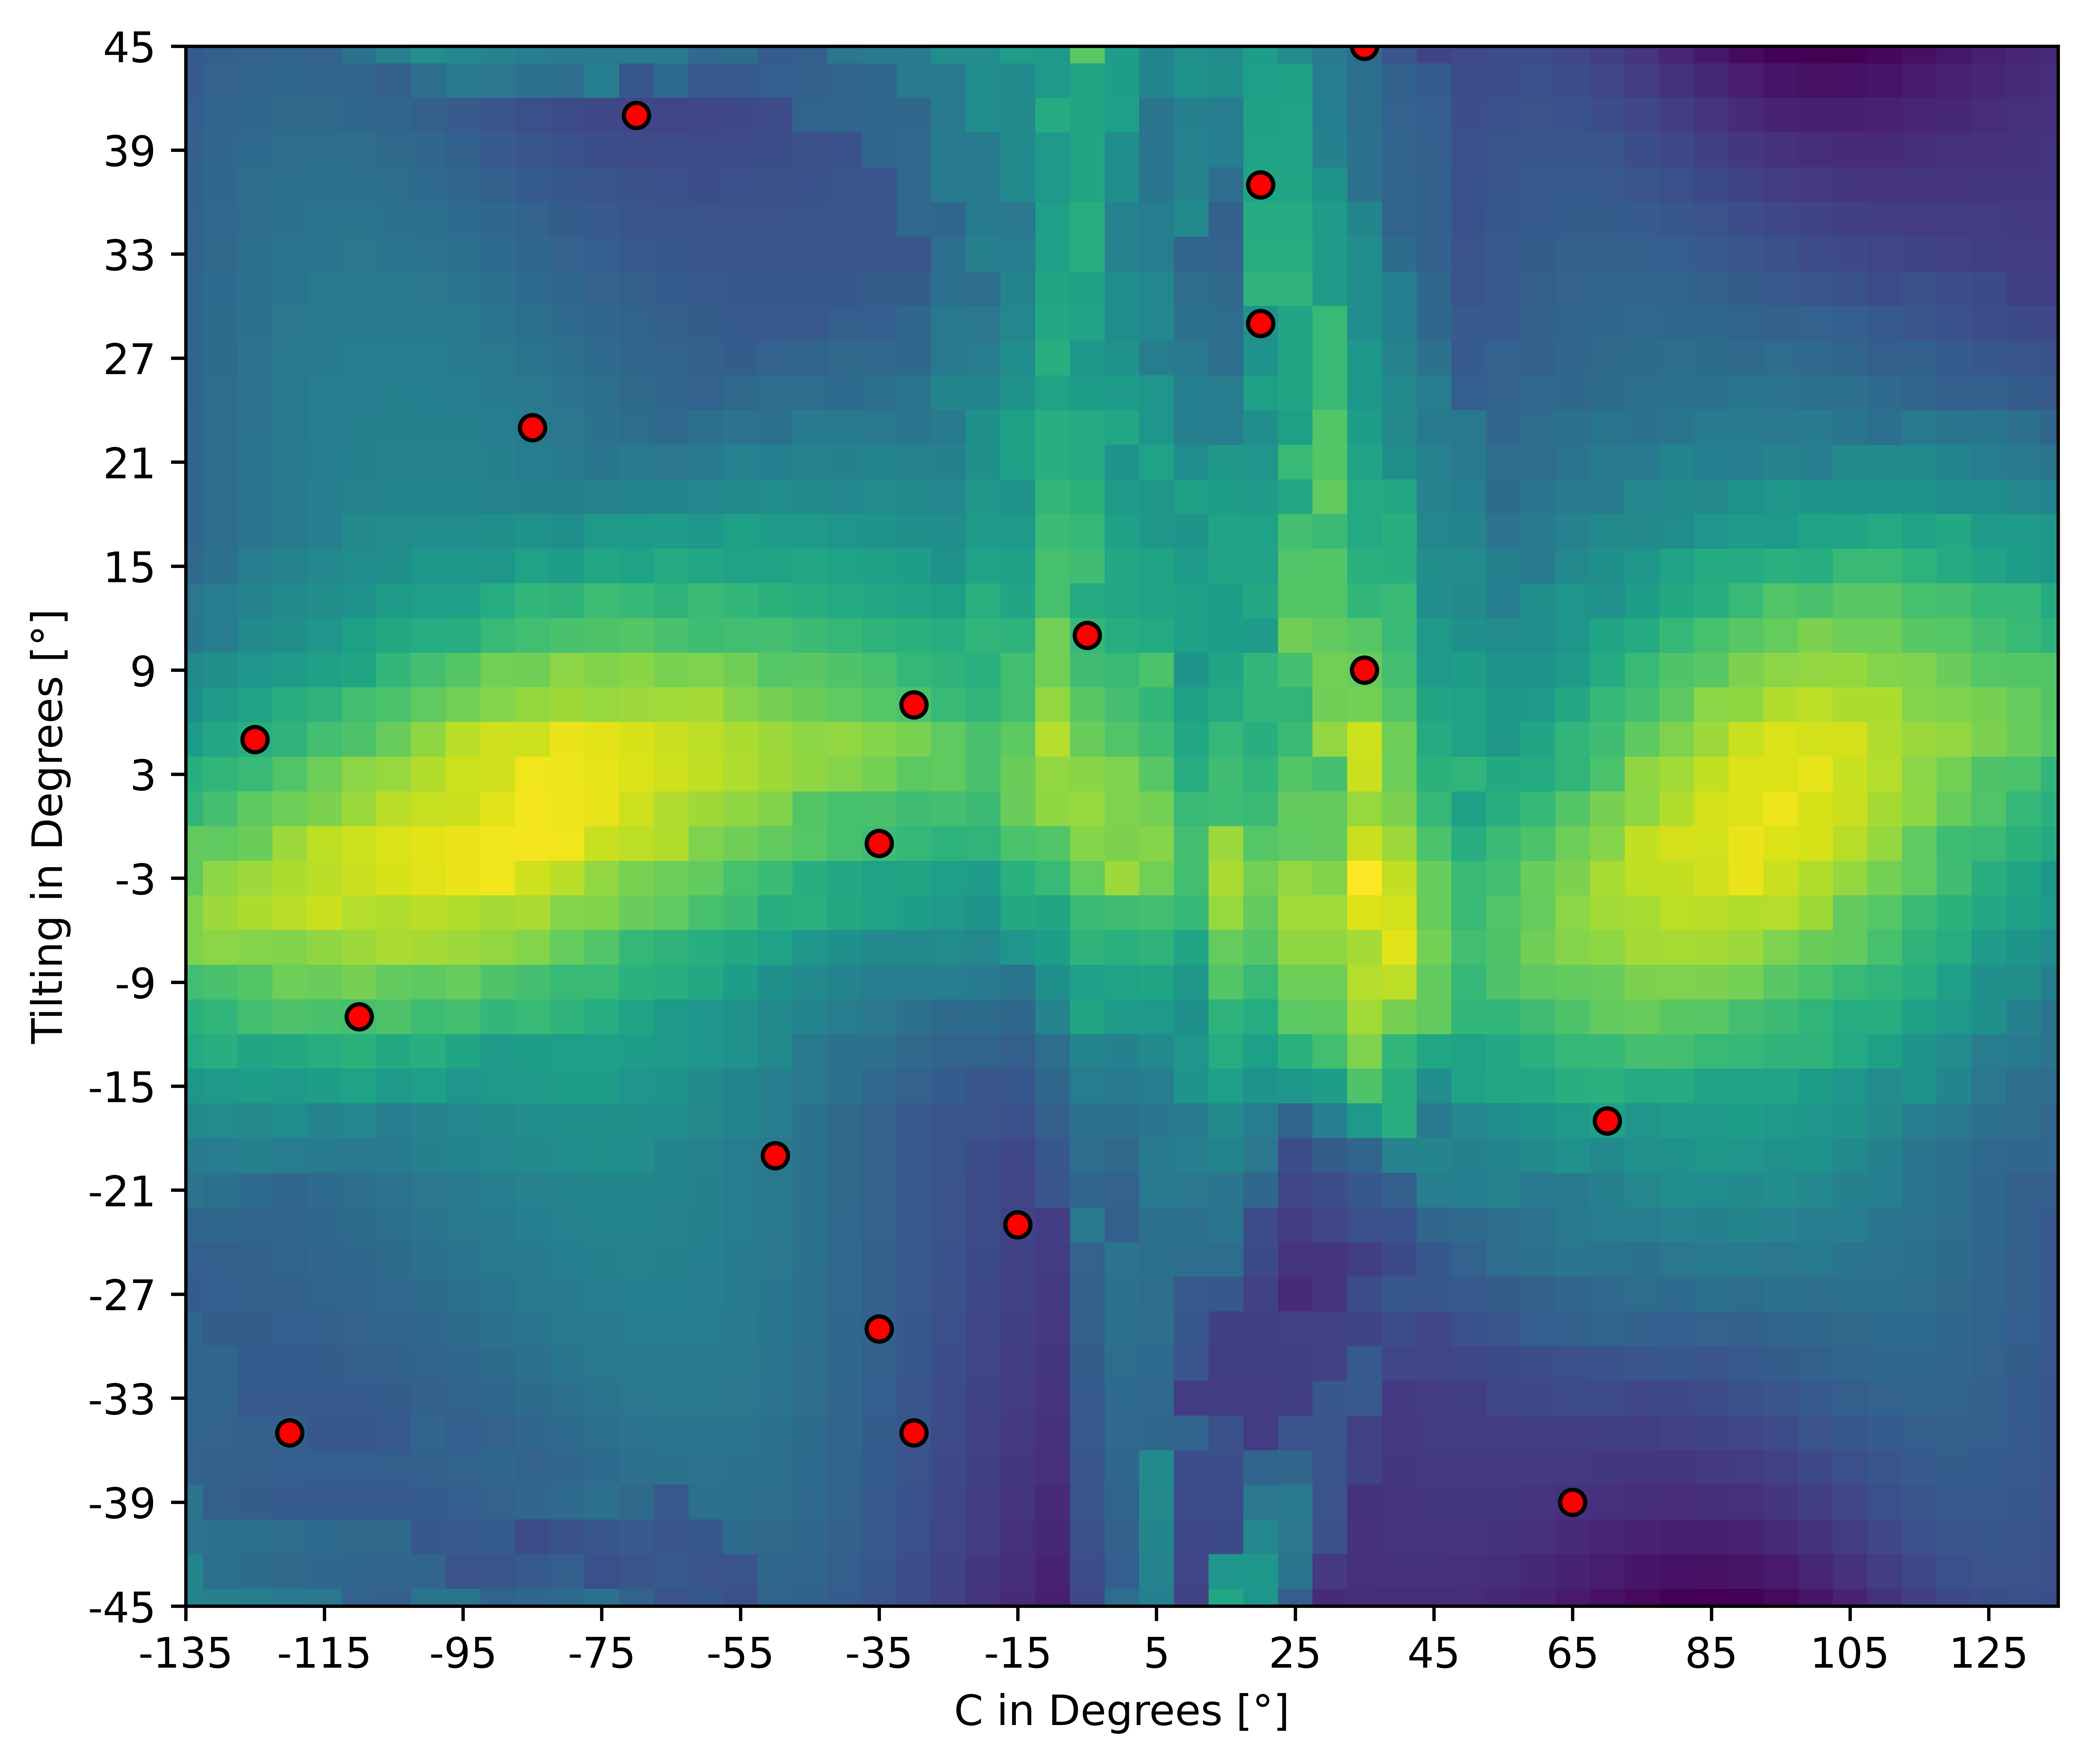
\includegraphics[width=0.7\textwidth]{figures/swarm/3_0.png}}
	\caption{Distributed of particles at their initial positions}
	\label{PSO_1}
\end{figure}



It is important to clarify that the individual particles in the \acrshort{PSO} algorithm do not have access to the entire global score matrix. The visualization of the global score matrix is only provided for the benefit of the human reader to aid in understanding. In reality, each particle only has knowledge of the global score at its own position. The particles update their positions iteratively by comparing their positions with each other. Each particle determines a new position based on the best score observed so far by all particles and the best score observed by itself. 

Figures \ref{2} to \ref{5} demonstrate the convergence of the particles towards the maximum global score. This convergence is achieved within 5 iterations. It is noteworthy that the best position of all 5 particles corresponds to the global maximum, as discussed in Chapter \ref{2RDOF}. This example highlights the ability to explore a high-dimensional space without the need to compute all possible combinations.


\begin{figure}[H]
	\centering
	\begin{minipage}{0.5\textwidth}
		\includegraphics[width=\textwidth]{figures/swarm/3_2.png}
		\caption{PSO Iteration 2 on toolpath 3}
		\label{2}
	\end{minipage}\hfill
	\begin{minipage}{0.5\textwidth}
		\includegraphics[width=\textwidth]{figures/swarm/3_3.png}
		\caption{PSO Iteration 3 on toolpath 3}
		\label{3}
	\end{minipage}\par
\end{figure}	


\begin{figure}[H]	
		\centering
	\begin{minipage}{0.5\textwidth}
		\includegraphics[width=\textwidth]{figures/swarm/3_4.png}
		\caption{PSO Iteration 4 on toolpath 3}
		\label{4}
	\end{minipage}\hfill
	\begin{minipage}{0.5\textwidth}
		\includegraphics[width=\textwidth]{figures/swarm/3_5.png}
		\caption{PSO Iteration 5 on toolpath 3}
		\label{5}
	\end{minipage}\par
\end{figure}
\newpage
One important consideration in this test is, that the scores have already been calculated. The global score matrix is determined by evaluating all possible combinations of different boundary conditions. However, in the intended scenario where this method is used to find the optimal boundary condition, such a pre-calculated matrix does not exist.

Therefore, in each iteration, the scores of the individual particle positions need to be compared relative to each other, taking into account the previous iterations. This process is illustrated in Figure \ref{swarmloop}. Initially, a predetermined number of particles is randomly placed on the plane, with the X and Y values representing the selected boundary conditions. For each selected boundary condition, the joint angles are calculated using the inverse kinematic approach. The analyzed process variables are then extracted and the joint angles are stored. The score for each current position is calculated relative to all stored toolpaths.

It is possible that in an early iteration, a particle had a position with a significantly higher score compared to the other available toolpaths. Therefore, after each iteration, it is necessary to update the score of the particle's most optimal position as more boundary conditions are analyzed. This is done to ensure that a score, which may have been mistakenly chosen as the best, does not influence the subsequent search directions.

\begin{figure}[H]
	\centerline{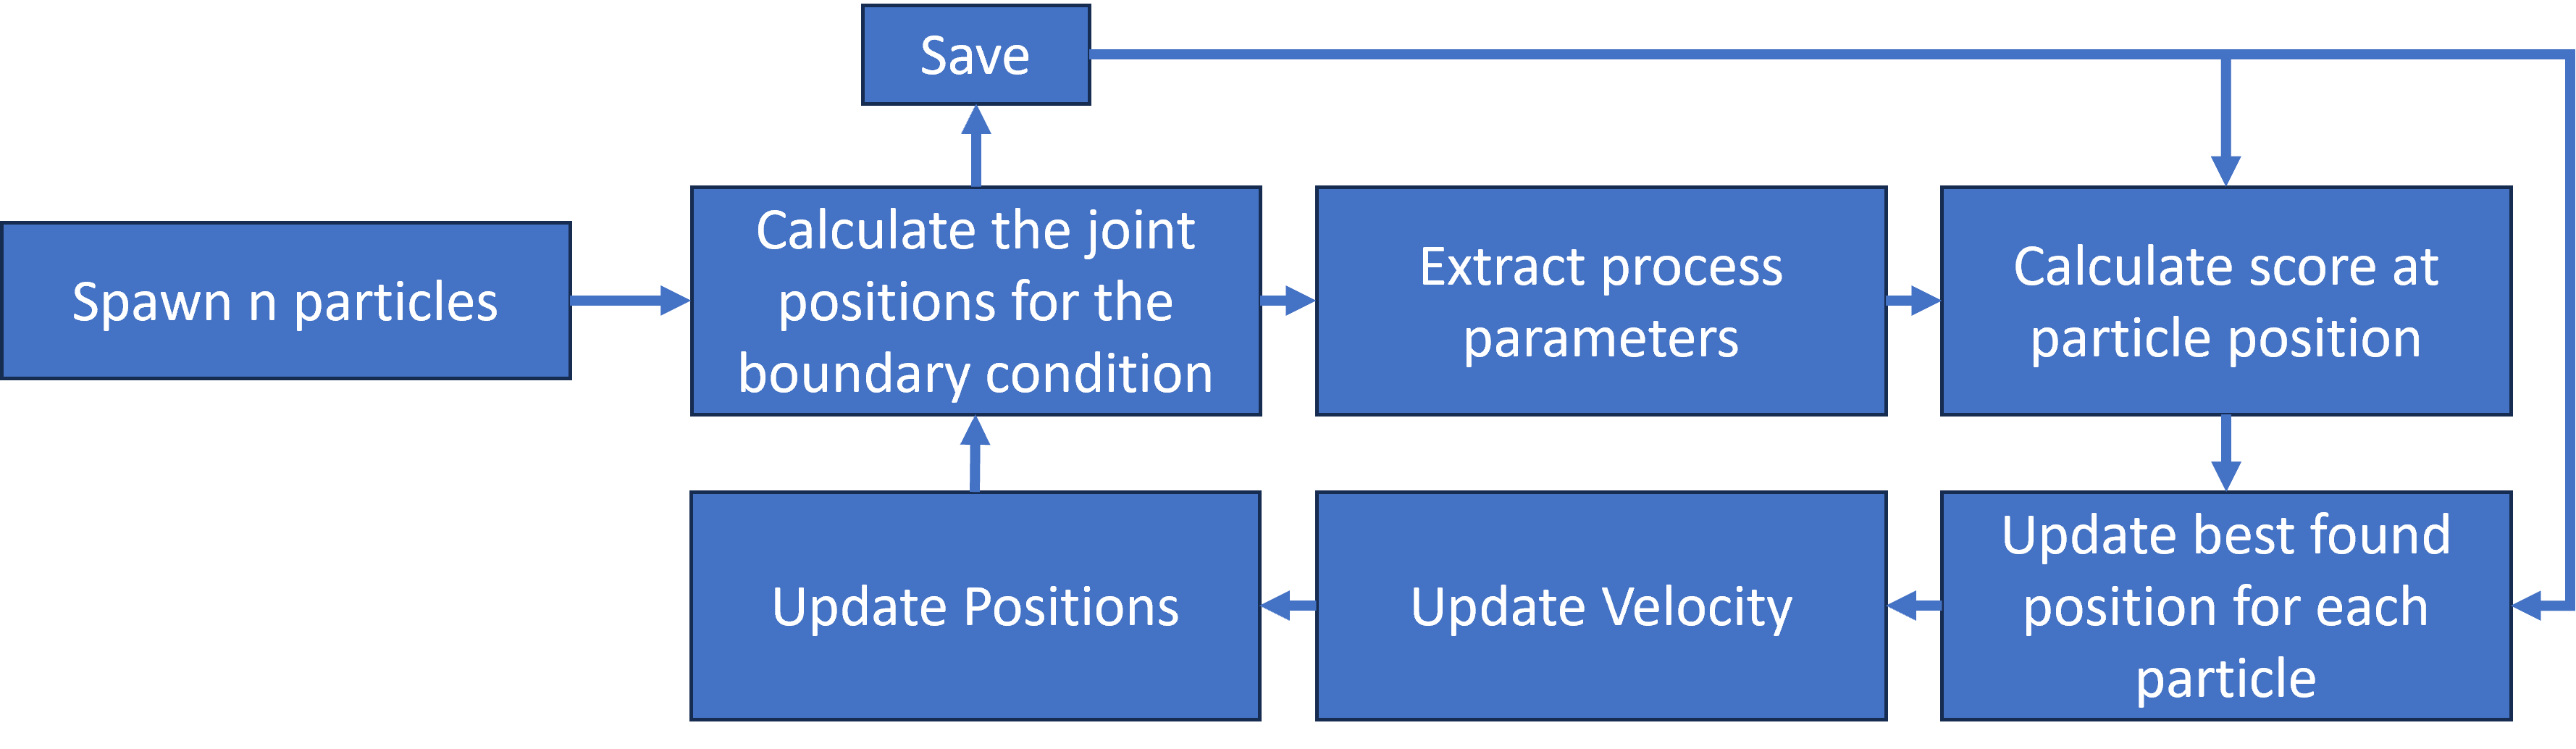
\includegraphics[width=1\textwidth]{figures/swarmloop.png}}
	\caption{PSO-Loop}
	\label{swarmloop}
\end{figure}

By utilizing this approach, the following results have been obtained. It is important to emphasize that the precalculated values of the global score matrix are not accessible to the \acrshort{PSO} algorithm. They are only used for evaluating the behavior of the particles and aiding in visualization. Figures \ref{1_true} to \ref{4_true} illustrate the evolution of the individual particles. The green circle represents the overall best position discovered by the particles up to that point
\newpage

\begin{figure}[H]
	\centering
	\begin{minipage}{0.5\textwidth}
		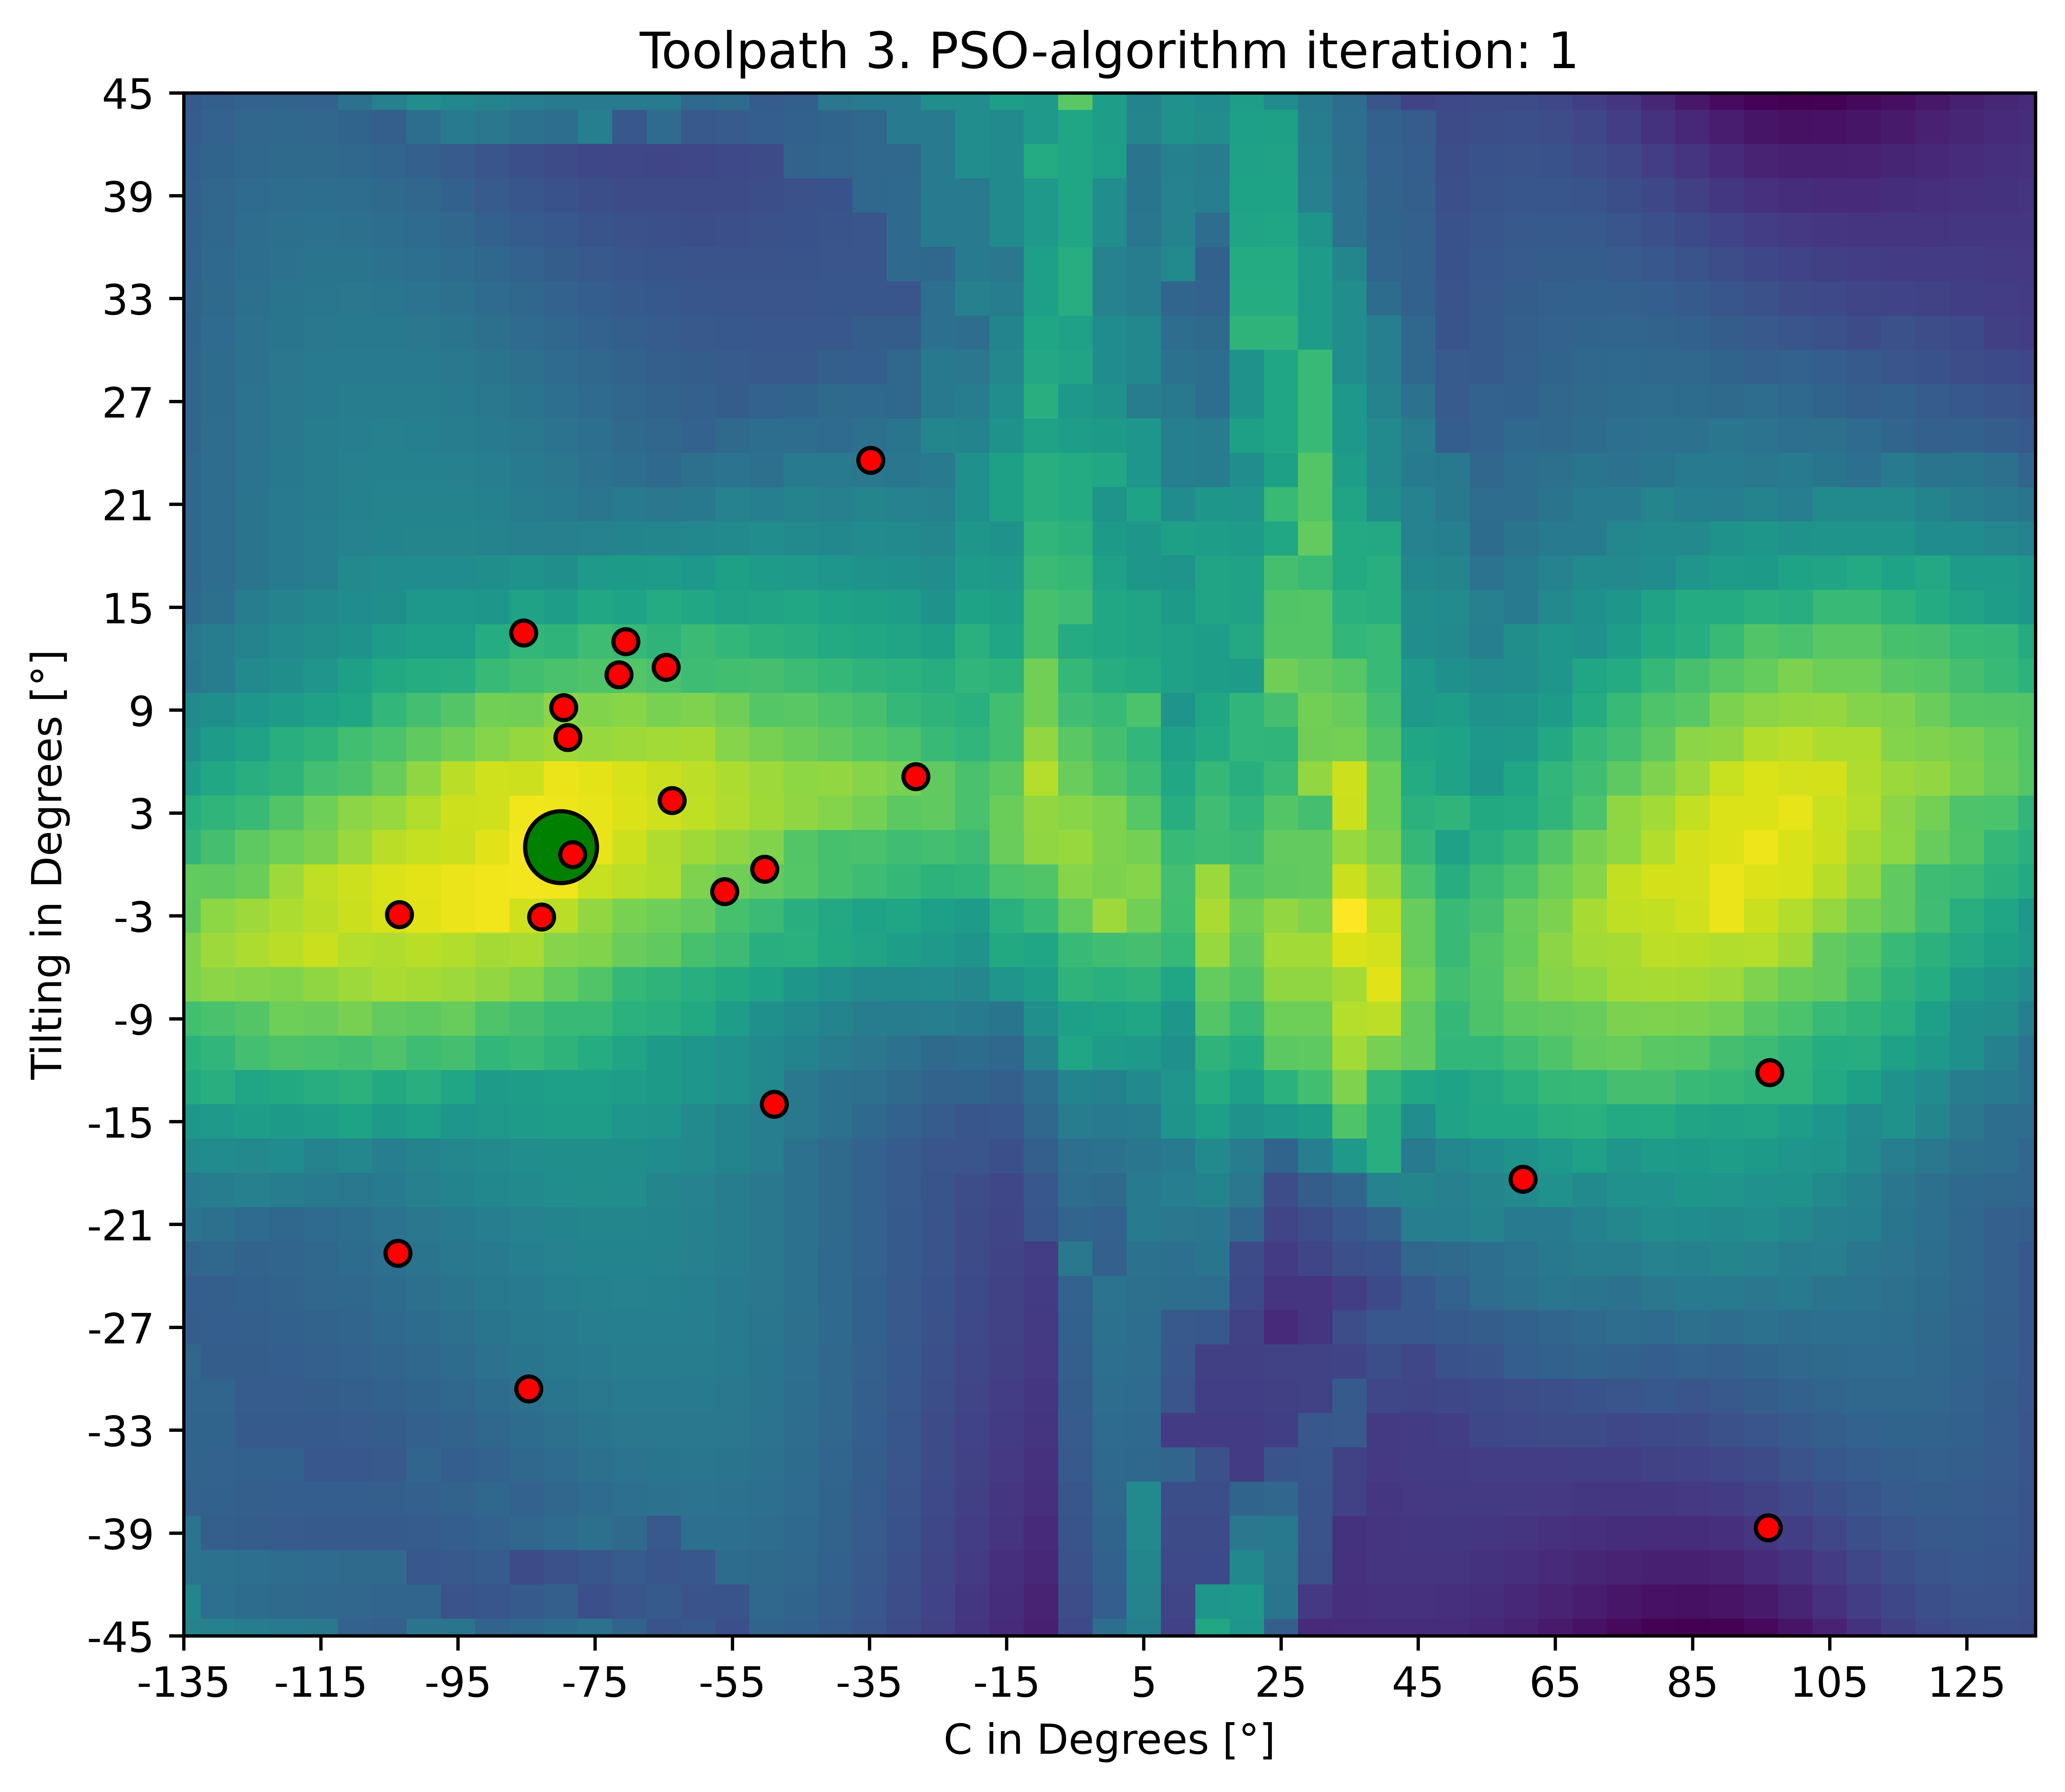
\includegraphics[width=\textwidth]{figures/swarm_true/3_1.png}
		\caption{PSO Iteration 1 on toolpath 3}
		\label{1_true}
	\end{minipage}\hfill
	\begin{minipage}{0.5\textwidth}
		\includegraphics[width=\textwidth]{figures/swarm_true/3_2.png}
		\caption{PSO Iteration 2 on toolpath 3}
		\label{2_true}
	\end{minipage}\par
\end{figure}	

\begin{figure}[H]	
	\centering
	\begin{minipage}{0.5\textwidth}
		\includegraphics[width=\textwidth]{figures/swarm_true/3_3.png}
		\caption{PSO Iteration 3 on toolpath 3}
		\label{3_true}
	\end{minipage}\hfill
	\begin{minipage}{0.5\textwidth}
		\includegraphics[width=\textwidth]{figures/swarm_true/3_4.png}
		\caption{PSO Iteration 4 on toolpath 3}
		\label{4_true}
	\end{minipage}\par
\end{figure}

The backtracking comparison of all previously visited positions by the particles is clearly evident in the movement of the green dot, which represents the best position found so far. As more points are visited by the particles, the calculation of the best boundary conditions improves. Even without the precalculated global score matrix, the particles are able to converge to the global optimum.
Figure \ref{5_true} illustrates the positions of the particles after the fifth and final iteration.
\newpage
\begin{figure}[H]
	\centerline{\includegraphics[width=0.8\textwidth]{figures/swarm_true/3_5.png}}
	\caption{PSO iteration 5 on toolpath 3}
	\label{5_true}
\end{figure}



The same optimization process can be applied to toolpath 1 and toolpath 2. The same process variables and weights are selected as for toolpath 3 (see Table \ref{PP_2}). Once again, 20 particles are analyzed over 5 iterations. Figures \ref{tp1_0} through \ref{tp1_5} depict the positions of the particles after the first and final iteration when analyzing the first toolpath, while Figures \ref{tp2_0} and \ref{tp2_5} showcase the initial and final positions of the particles when analyzing the second toolpath. In both cases, the PSO algorithm successfully converges very closely towards the optimal boundary condition.
\newpage
	
\begin{figure}[H]	
	\centering
	\begin{minipage}{0.5\textwidth}
		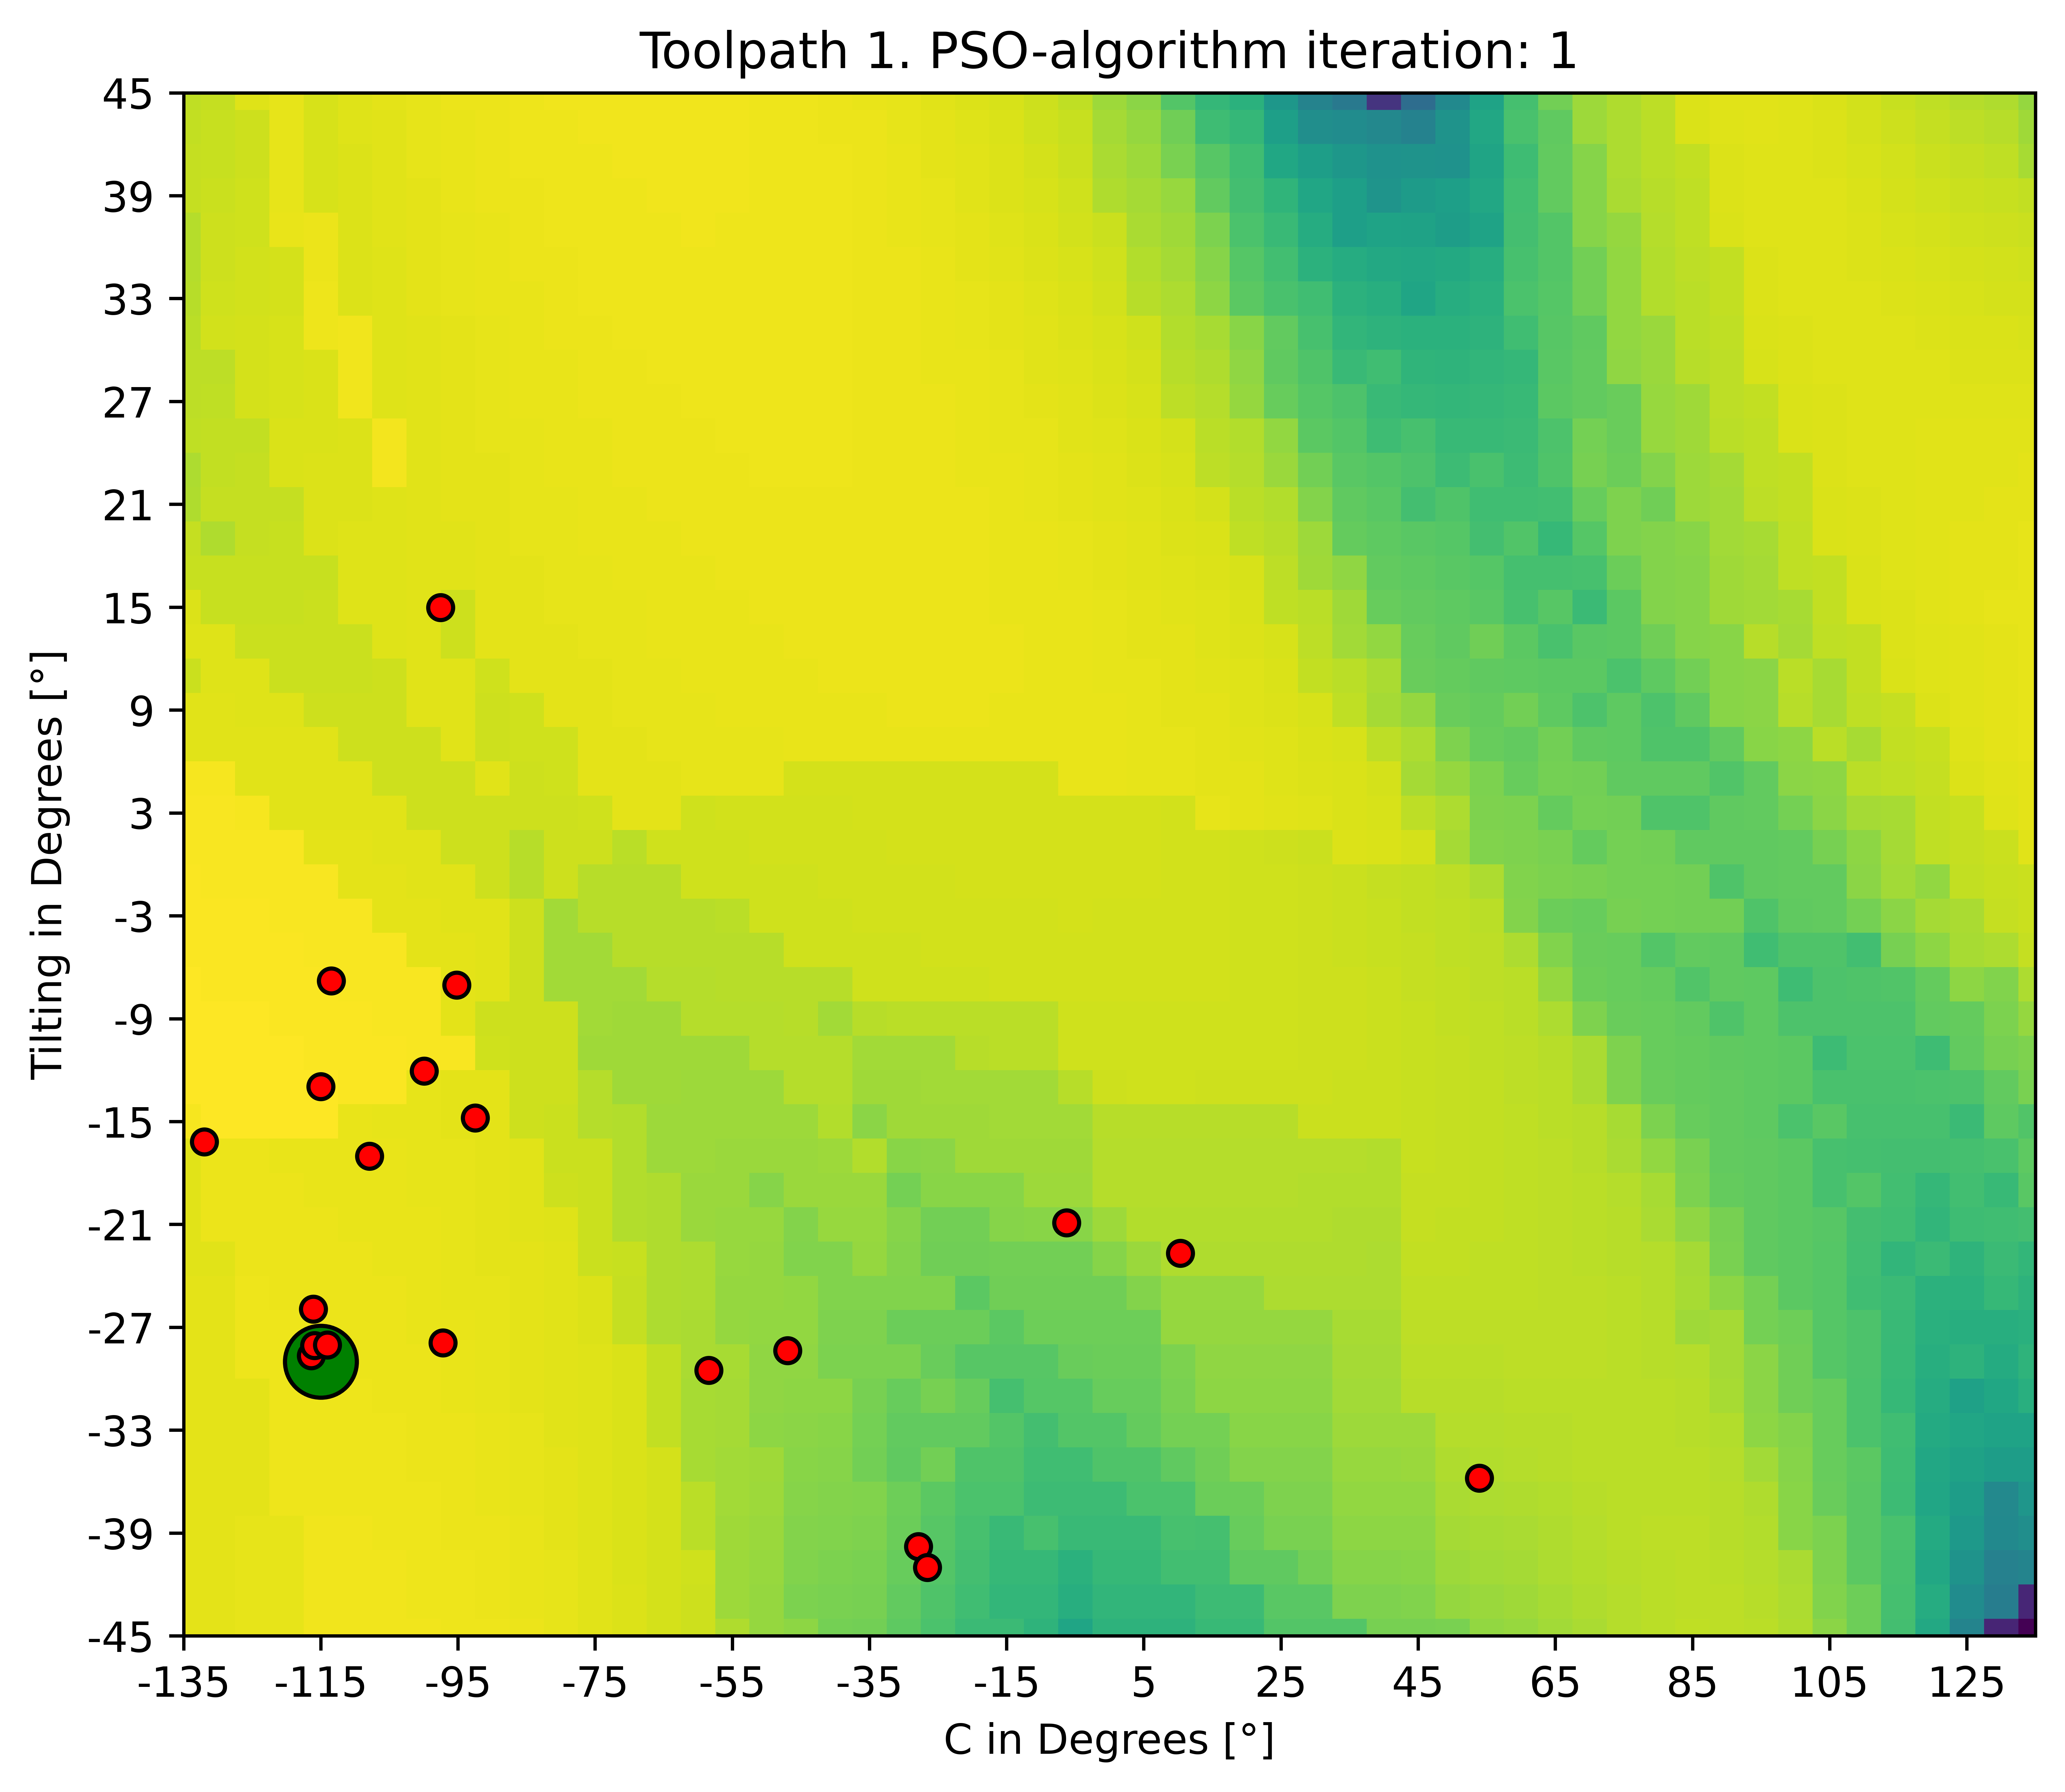
\includegraphics[width=\textwidth]{figures/swarm_true/1_1.png}
		\caption{PSO Iteration 1 on toolpath 1}
		\label{tp1_0}
	\end{minipage}\hfill
	\begin{minipage}{0.5\textwidth}
		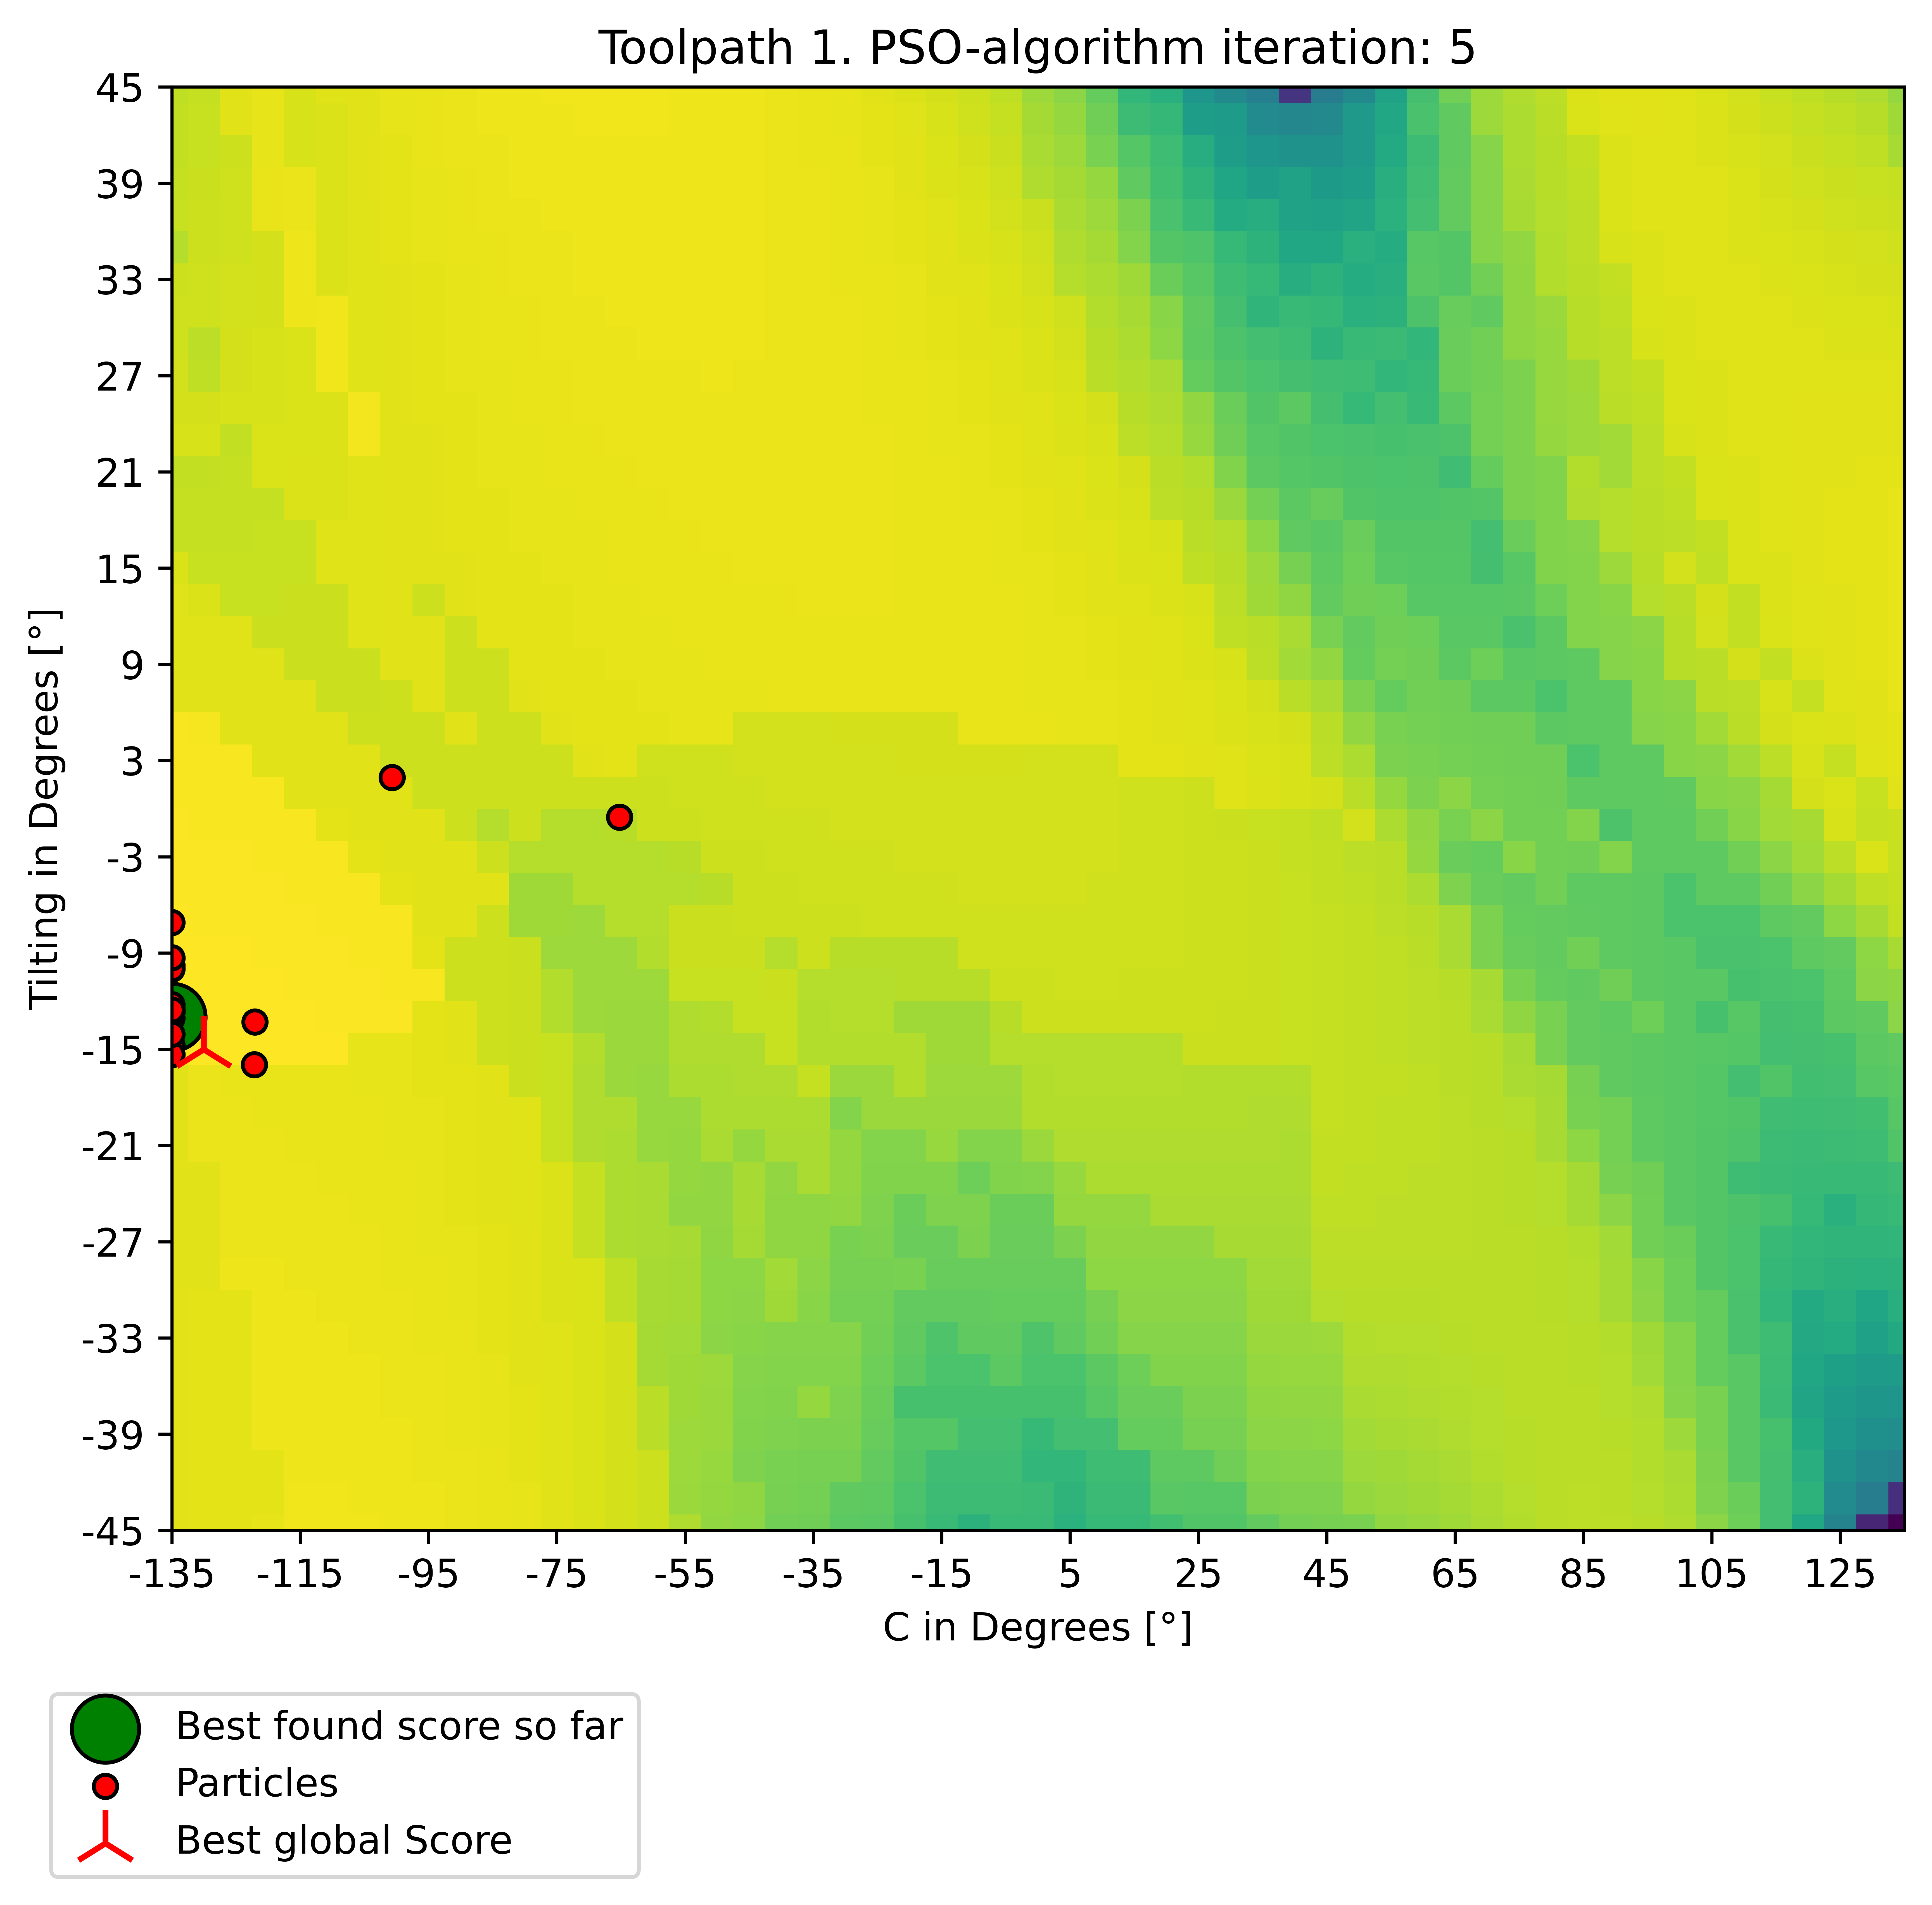
\includegraphics[width=\textwidth]{figures/swarm_true/1_5.png}
		\caption{PSO Iteration 5 on toolpath 1}
		\label{tp1_5}
	\end{minipage}\par
\end{figure}


\begin{figure}[H]	
	\centering
	\begin{minipage}{0.5\textwidth}
		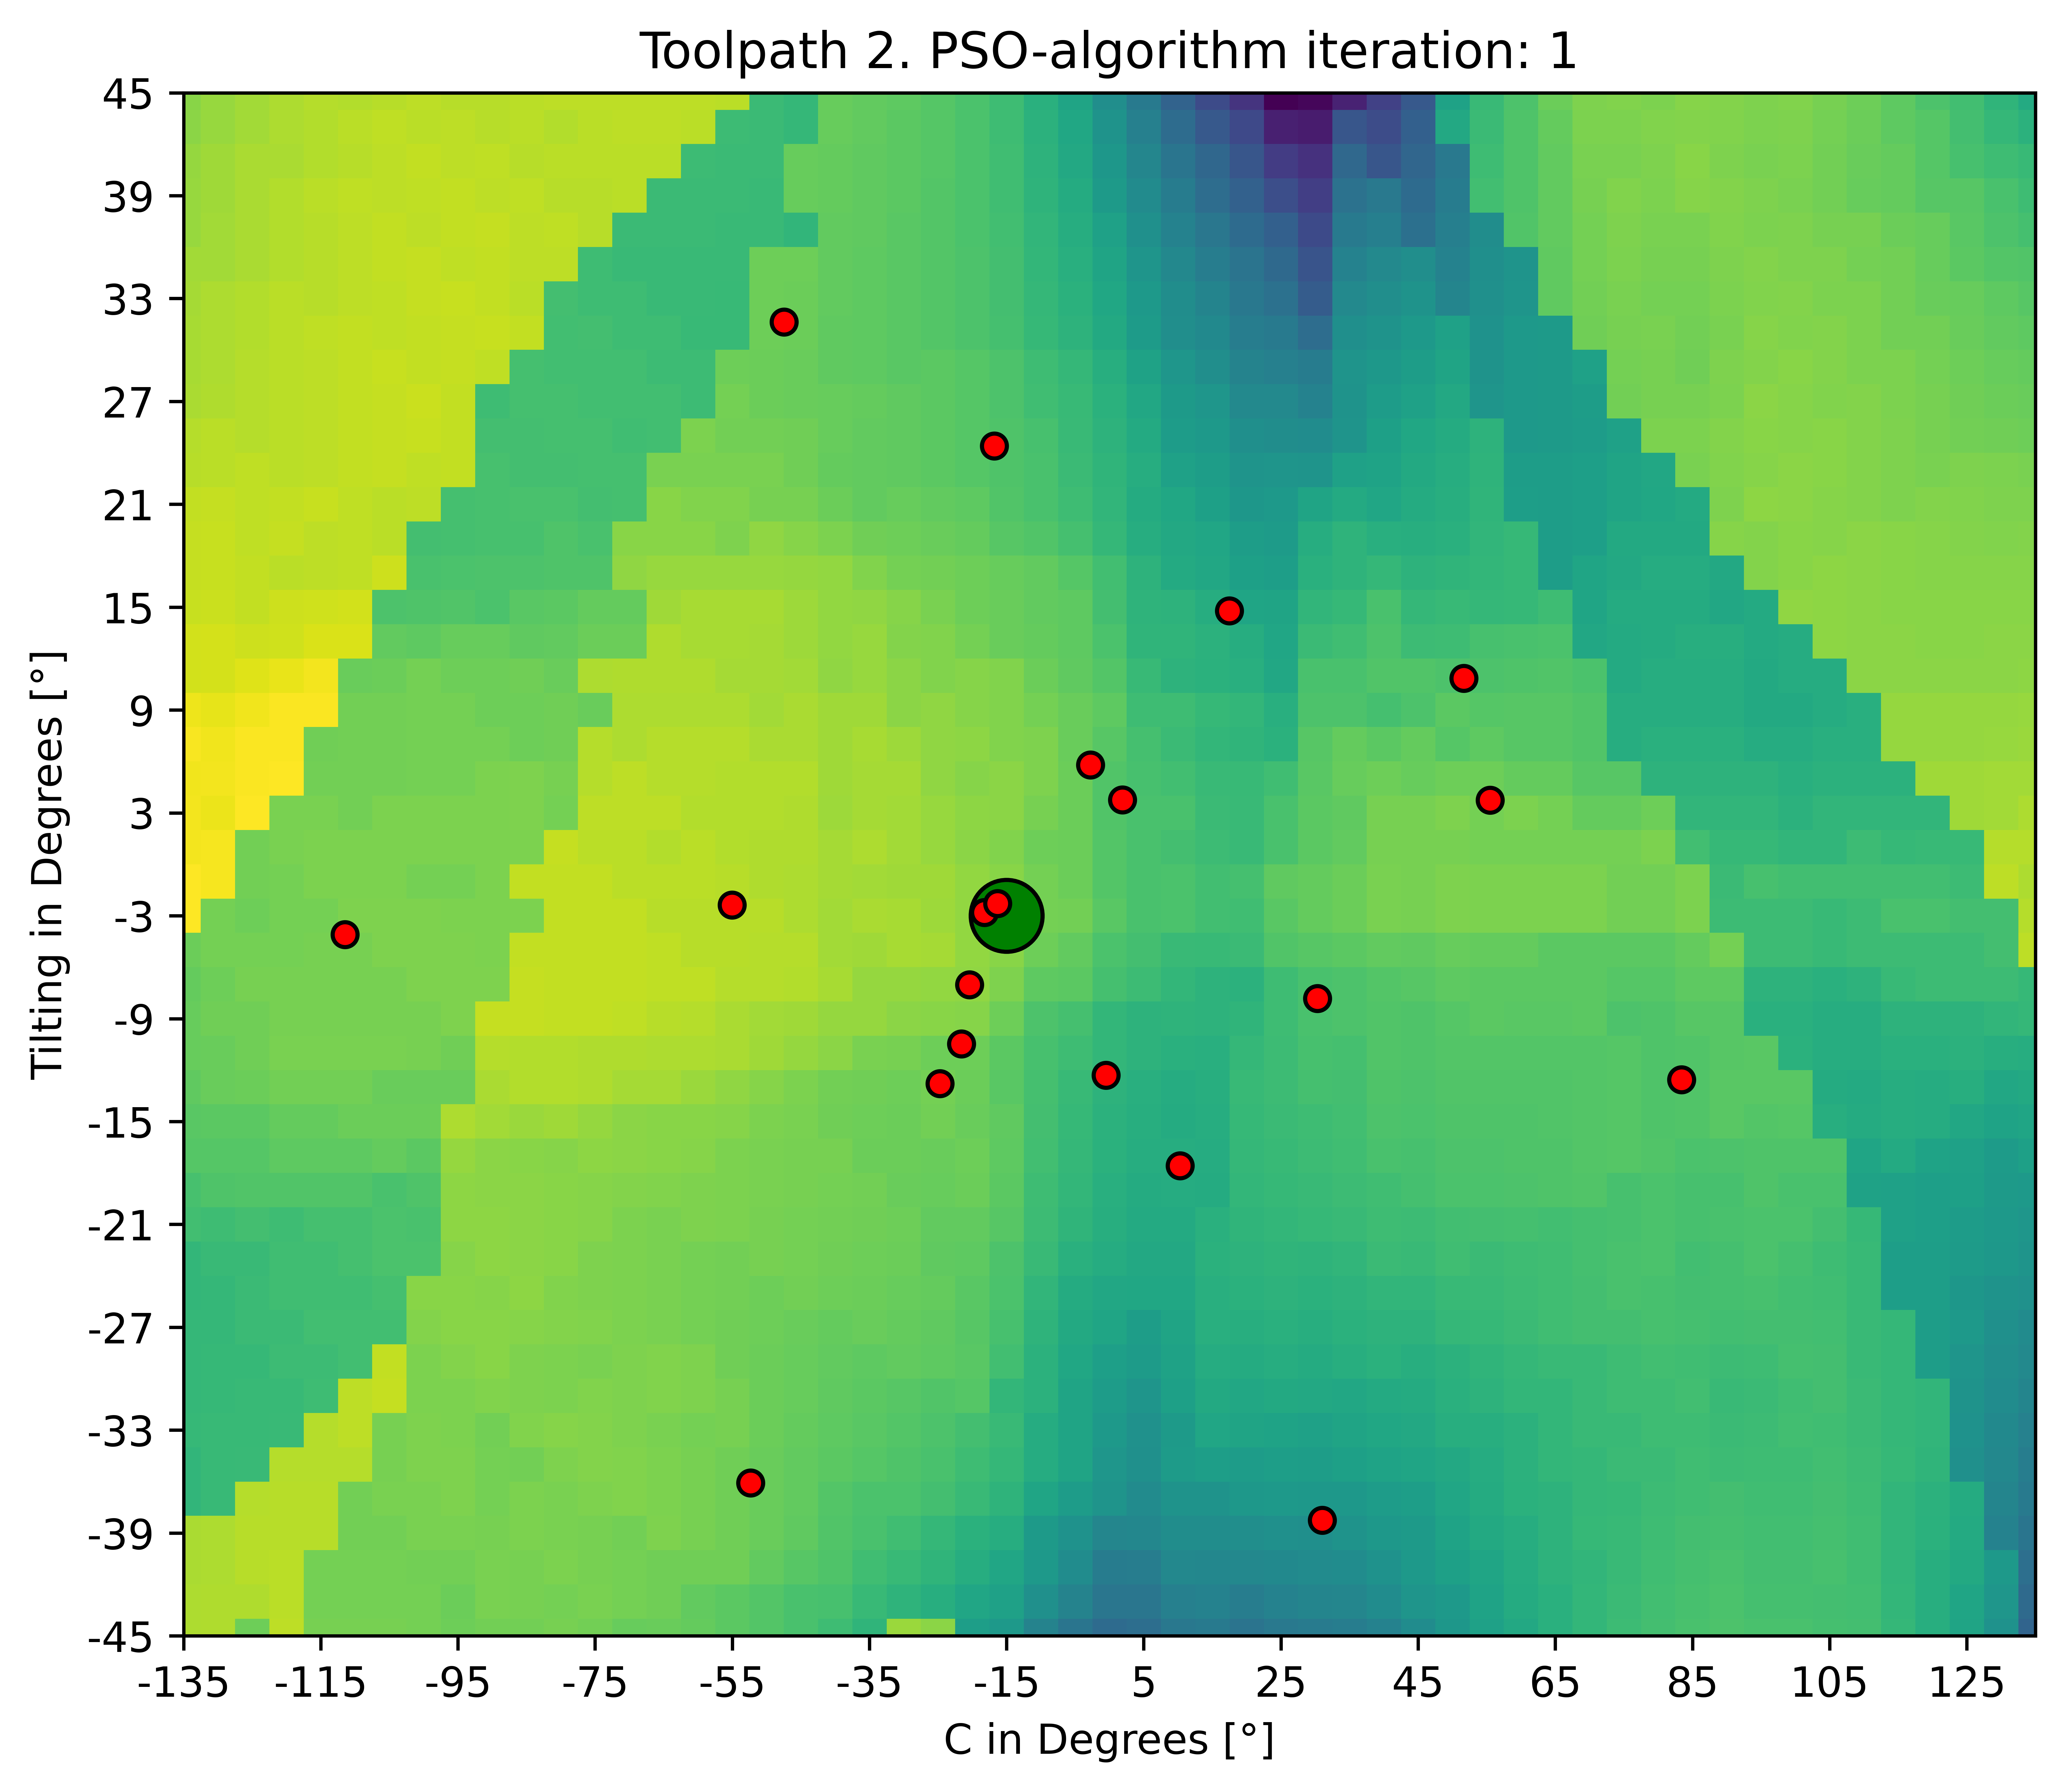
\includegraphics[width=\textwidth]{figures/swarm_true/2_1.png}
		\caption{PSO Iteration 1 on toolpath 2}
		\label{tp2_0}
	\end{minipage}\hfill
	\begin{minipage}{0.5\textwidth}
		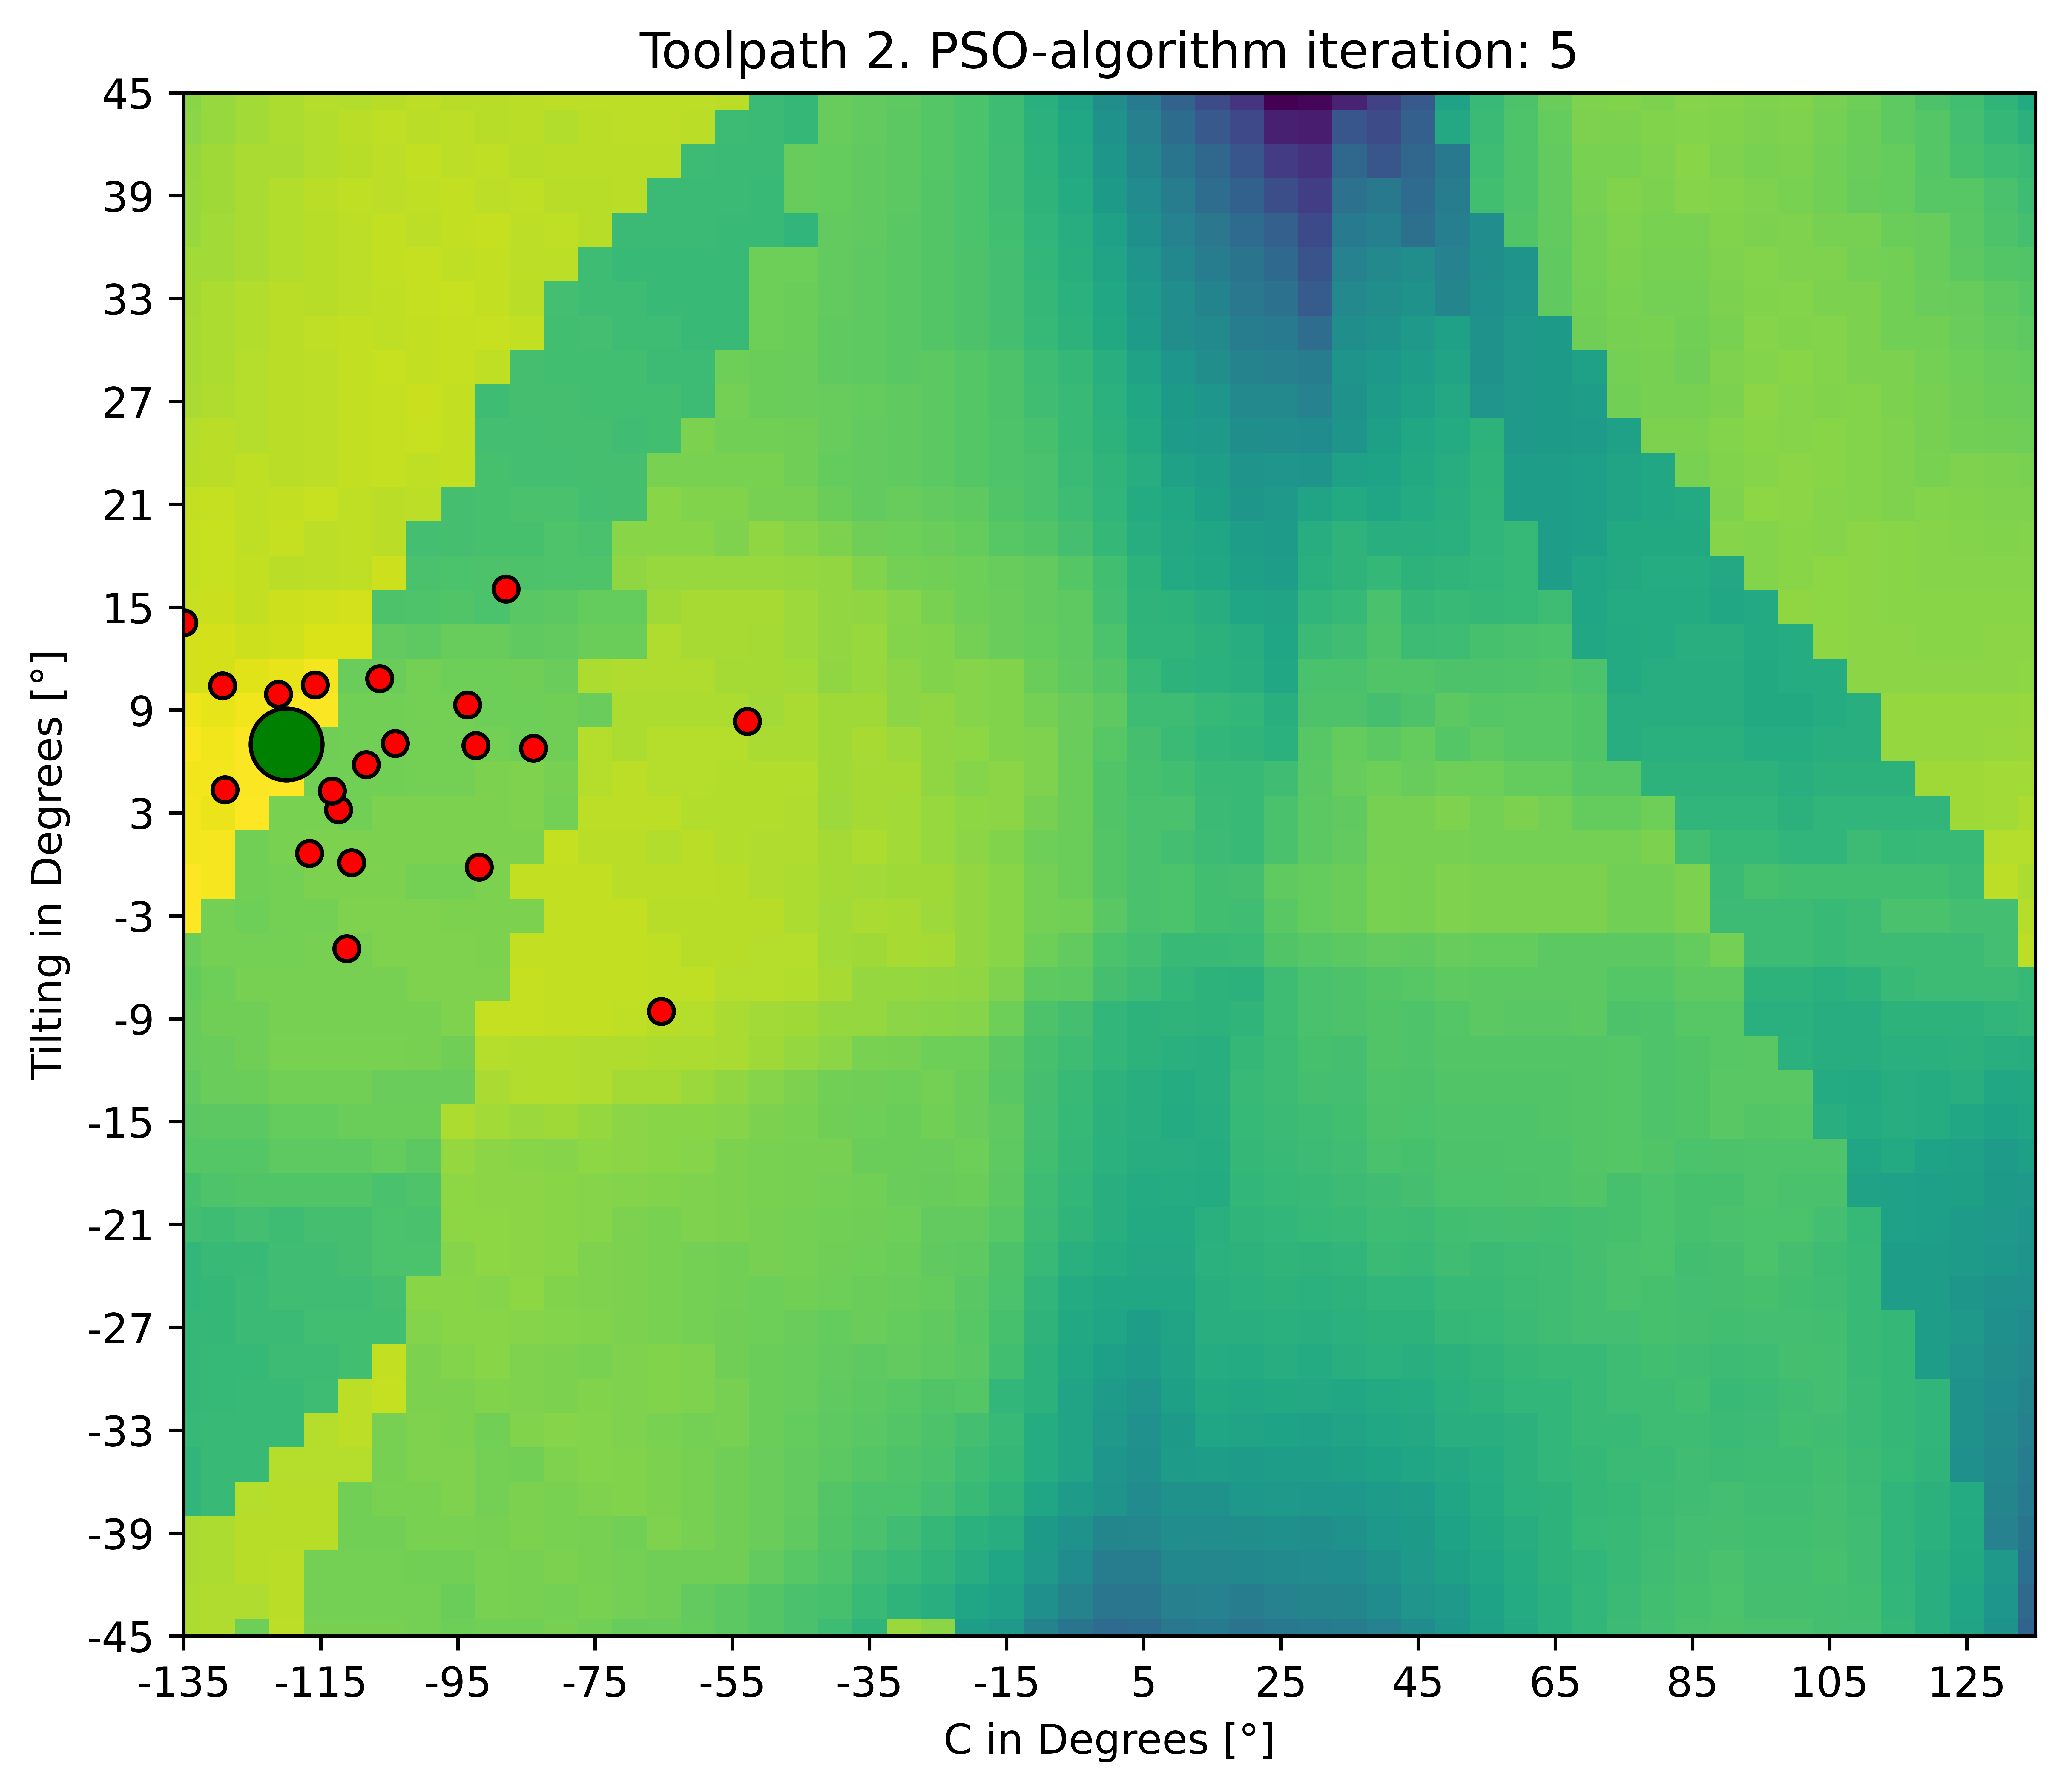
\includegraphics[width=\textwidth]{figures/swarm_true/2_5.png}
		\caption{PSO Iteration 5 on toolpath 2}
		\label{tp2_5}
	\end{minipage}\par
\end{figure}



\newpage
\section{Analysis and Discussion of the Results}%
In the following, the results are analyzed in detail and critically discussed.

\subsection{Summary and Analysis of the Results}
When analyzing only one redundant \acrshort{DoF}, specifically the rotation around the Z-axis (see Figure \ref{GS1}, Figure \ref{TP2_combi}, and Figure \ref{TP3_combi}), it becomes evident that there is significant potential for improvement. In this initial test, the process variables "direction changes in all joints," "total travel in all joints," and "acceleration in joint 1" are analyzed. The local score for "total travel in all joints" and "acceleration in joint 1" both exhibit a very continuous change over the entire range of the analyzed rotation. This characteristic is a clear indication that optimization algorithms are a reasonable choice for finding the optimal boundary condition.

To further validate the proposed method for analyzing process variables, a production-grade G-Code is examined (see Figure \ref{LS4}). This G-Code consists of 28,000 coordinates and takes significantly longer to analyze. The resulting comparison of all possible values for the redundant \acrshort{DoF} shows a fairly smooth curve of the global score. It is important to note that the local score for the direction changes in all analyzed toolpaths is not as smooth as the other analyzed variables.


When considering the scenario where two \acrshort{DoF} can be set, it is observed that toolpath 1 and toolpath 2 have very similar boundary conditions for the global optimum (see Figure \ref{best_2D_1} and Figure \ref{best_2D_2}). This suggests that these two toolpaths do not differ significantly from each other when considering the process variables alone. 

Analyzing the hyperplane of toolpath 1 (Figure \ref{best_2D_1}), it is clearly visible that most of the possible combinations result in a very high global score. The combinations that lead to a low local score form a ravine that is clearly visible on the right-hand side. In the case of toolpath~2 (Figure \ref{best_2D_2}), distinct streaks can be observed. The middle of the matrix represents a continuous region, while multiple discontinuities occur on the sides. Toolpath 3 (Figure \ref{best_2D}) exhibits an almost symmetrical hyperplane. Two local optima are visible on the left and right sides, while the middle part consists of a jagged area with many non-smooth jumps. It is worth noting that the calculation of each individual global score matrix takes approximately 1 hour.


Based on the results obtained from the \acrshort{PSO} algorithm (see Figure \ref{5_true}), it can be concluded that achieving a close-to-optimal result is feasible when the global score matrix yields smooth surfaces. By implementing this approach, a significant reduction in computation time is possible. Instead of calculating the entire matrix, only 100 toolpaths need to be computed using the inverse kinematics algorithm, resulting in a computation time of just 15 minutes.

The number of particles is selected to be as high as possible while also considering the computational costs. Rather than increasing the number of particles, the number of iterations is set to 5 in order to facilitate convergence towards the global optima. The results clearly show that such a convergence is possible.


%NO \acrshort{CAM} EXPLAIN








\subsection{Discussion of the Results}%


Even though the results show a very promising outcome, it is necessary to consider some additional factors. One of the most obvious elements is that only three artificial and one production-grate toolpaths are analyzed. To validate this method in detail, it is necessary to use more real-life production G-code with correctly modeled robotic systems and analyze whether it can be optimized. It should be noted that this work only provides a limited excerpt and does not analyze complex multi-axis operations, which are a significant advantage and building block of the \acrshort{WAAM} process.

The selected inverse kinematics algorithm is not designed for optimal high-performance calculations, making it infeasible to use when dealing with toolpaths that have millions of coordinates. Additionally, the algorithm calculates the joint position numerically rather than analytically, which can result in unexpected robot poses. \acrshort{CAM} software such as \textit{Siemens NX} or \textit{Master CAM} offer additional options for inverse kinematics that can be used to fine-tune the behavior of the robot.

When analyzing multiple process variables, it is not guaranteed that the resulting surface will be smooth and optimal for the selected optimization algorithm. Additionally, when working with a \acrshort{PSO} algorithm, the final result strongly depends on the initial distribution of the particles. If the optimum is a very tight and sharp spike, the probability of finding the optimal boundary condition is significantly lower. This is particularly true in systems with 3 or more redundant \acrshort{DoF}, where simple optimization algorithms can lead to suboptimal results or require unfeasibly long computation times. When implementing the \acrshort{PSO} algorithm, 20 particles over 5 iterations are analyzed. In future work, it is necessary to analyze how a increase in population size will improve the convergence rate. 

When analyzing Figure \ref{GS1}, Figure \ref{TP2_combi}, and Figure \ref{TP3_combi}, it becomes evident that the best boundary conditions for the highest global score are very similar. Both toolpath 1 and 2 have an optimum of -120°, while toolpath 3 has an optimum at -90°. This suggests that there could be an optimal robot configuration that is applicable to any toolpath.

In general, the presented methodology does provide a solid basis as a proof of concept for the proposed method. However, additional implementations and test are necessary for it to be feasible in an industrial environment.
